%% =====================================================================
%%  A Parameter-Efficient Dual-Head Oral Disease Classifier
%%  IEEE journal-style manuscript.
%%
%%  BUILD (run from this directory):
%%     pdflatex main  ->  bibtex main  ->  pdflatex main  ->  pdflatex main
%%  IEEEtran.cls and IEEEtran.bst are bundled in this directory, so the
%%  paper compiles even though the local TeX Live does not have them
%%  installed system-wide.  Compile FROM the paper/ directory.
%% =====================================================================
\documentclass[journal,a4paper]{IEEEtran}

% ---- packages (all confirmed present in the local TeX Live 2025) -----
\usepackage{graphicx}      % figure inclusion
\usepackage{amsmath}       % math
\usepackage{amssymb}       % math symbols
\usepackage{array}         % extended column specifiers
\usepackage{tabularx}      % width-balanced tables
\usepackage{dcolumn}       % decimal-point-aligned numeric columns
\usepackage[hidelinks]{hyperref}   % hyperlinks (hidelinks => no xcolor needed)

\interdisplaylinepenalty=2500       % IEEEtran recommendation (load after amsmath)

%  NOTE: the bundled IEEEtran.cls carries a local patch that swaps the
%  Times/Helvetica/Courier font defaults for Computer Modern, because
%  this machine's TeX Live lacks the Times metrics.  See IEEEtran.cls
%  near line 494.  Nothing else in the preamble is affected.

\graphicspath{{figures/}}
\DeclareGraphicsExtensions{.pdf,.png}

% ---- decimal-aligned numeric column type for the result tables -------
%      usage in a tabular preamble:  d{4}  -> aligns numbers on the dot,
%      4 digits after the point.
\newcolumntype{d}[1]{D{.}{.}{#1}}

% ---- small helpers ---------------------------------------------------
\newcommand{\arrowto}{$\rightarrow$}        % Triplet -> SE cascade arrow

\begin{document}

\title{A Parameter-Efficient Dual-Head Oral Disease Classifier with an
Ablation-Driven Triplet\arrowto{}SE Attention Cascade}

\author{First~Author,~Second~Author,~and~Third~Author% TODO(user): real names
\thanks{Manuscript submitted \today.}% TODO(user): submission details
\thanks{The authors are with [Department], [Institution], [City], [Country]
(e-mail: corresponding.author@example.com).}}% TODO(user): affiliations

\maketitle

\begin{abstract}
Computer-aided diagnosis of oral disease has matured along two narrow tracks (binary malignant-versus-benign screening and pixel-level lesion segmentation), while multi-class subtype classification, the formulation most aligned with downstream clinical decision-making, remains comparatively under-explored, and the few existing multi-class systems rely on heavy ensembles whose architectural choices are not justified by ablation. This paper proposes a parameter-efficient five-stage Convolutional Neural Network (CNN) backbone, \emph{Custom EfficientNet~V2}, in which the standard Block-4 of EfficientNetV2-B0 is replaced by a domain-tuned \emph{AttentionHub} module. A second variant, \emph{AttentionHub-v2}, is then derived: a sequential cascade of Triplet Attention followed by Squeeze-and-Excitation (SE), whose design is forced by a systematic seven-cell ablation of the v1 hub. The ablation reveals a \emph{role-complementarity principle}. Pairing Triplet (a cross-dimensional spatial attention) with any module that also exercises a spatial role, namely the Bottleneck Attention Module (BAM) or Efficient Multi-scale Attention (EMA), regresses subtype accuracy to a recurring $98.36\,\%$ sub-baseline ceiling. Pairing Triplet with a \emph{purely} channel-wise partner (Kolmogorov-Arnold Network attention (KAN) or SE) instead lifts performance to $99.45\,\%$ and $99.51\,\%$ respectively. Trained from scratch under a single matched recipe and benchmarked against nine standard CNN and Transformer baselines on a seven-class oral disease dataset combined with a binary benign-versus-malignant split, the proposed model attains $99.06\,\%$ binary and $99.51\,\%$ subtype accuracy, the highest subtype score in the benchmark, at only $4.79$~M parameters and $0.493$~GFLOPs, $2.1\times$ smaller than EfficientNet~V2-B2 and $5.0\times$ smaller than Inception~V3, the two strongest baselines. Gradient-weighted Class Activation Mapping++ (Grad-CAM++) and Local Interpretable Model-Agnostic Explanations (LIME) panels indicate that the network attends to lesion tissue rather than to incidental visual artifacts. The complete experimental package, comprising nine matched baselines, seven attention ablations, dual-task evaluation, and per-model interpretability artifacts, is released to support reproducibility.

\end{abstract}

\begin{IEEEkeywords}
Oral disease classification, attention mechanisms, ablation study,
parameter-efficient architectures, EfficientNet, role-complementarity,
Grad-CAM++, LIME, dual-head multi-task learning, Triplet Attention,
Squeeze-and-Excitation.
\end{IEEEkeywords}

\section{Introduction}\label{sec:intro}

Oral diseases, including ulcerative, inflammatory, and
neoplastic lesions, present a complex visual challenge for automated
analysis. Conditions such as recurrent aphthous ulcer, oral lichen planus, and
squamous-cell carcinoma can share overlapping colour, texture, and boundary
cues at the image level, yet a single misclassification between a benign
inflammatory lesion and an early malignancy carries materially different
clinical consequences. A computer-aided diagnostic system must therefore solve
two related but distinct problems: identifying \emph{whether} a lesion is
malignant (binary screening) and identifying \emph{which} of several
visually similar conditions is present (multi-class subtyping). The second
problem is the one that most directly governs the choice of downstream
management pathway, and it is the focus of this paper.

Deep learning has matured rapidly in this domain. CNNs and, more recently,
Vision Transformers have produced strong binary screening
results~\cite{ref5,ref16,ref17} and several promising multi-class
systems~\cite{ref19,ref22}. Despite this progress, three persistent gaps remain
in the literature.

\emph{Gap~1: Binary formulations dominate.} Most published architectures
collapse oral pathology to a benign-versus-malignant decision. This formulation
is clinically insufficient when downstream treatment depends on differentiating
among multiple non-malignant conditions that visually mimic malignancy, since
ulcerative, inflammatory, and neoplastic lesions warrant different management
pathways.

\emph{Gap~2: Attention modules are stacked without ablation.} Modern
backbones routinely embed attention components such as Squeeze-and-Excitation
(SE), the Convolutional Block Attention Module (CBAM), the Bottleneck Attention
Module (BAM), Triplet Attention, Efficient Multi-scale Attention (EMA), and
Kolmogorov-Arnold Network attention (KAN), yet their individual and combined
contributions in the oral-disease setting are rarely measured. The literature
offers little guidance on which attention modules complement one another and
which conflict, and proposed architectures tend to inherit attention designs
from generic benchmarks rather than testing them on the target distribution.

\emph{Gap~3: Explainability evidence is sparse.} Few multi-class oral
disease studies present visual attention maps that demonstrate the model
attends to lesion tissue rather than to teeth, lip outlines, or lighting
artifacts. Absent such evidence, it is difficult to argue that a high-accuracy
model is also clinically defensible.

The present work addresses these three gaps directly. We make the following
four contributions.

\begin{enumerate}
  \item We design \textbf{Custom EfficientNet~V2}, a five-stage
  parameter-efficient backbone derived from EfficientNetV2-B0 in which the
  standard Block-4 is replaced by a domain-tuned \emph{AttentionHub} and the
  redundant Block-6 and convolutional head are removed, yielding a
  $4.79$~M-parameter, $0.493$~GFLOPs model.
  \item We perform a systematic \textbf{seven-cell ablation} of the
  AttentionHub spanning the \{BAM, Triplet, KAN\} singletons, all pairs, and
  the full triple, plus a no-attention control. From this ablation we derive a
  \textbf{role-complementarity principle}: pairing two spatial-role attention
  modules regresses the hub below its no-attention control, whereas pairing a
  spatial module with a purely channel-wise one is complementary. The principle
  is supported by the v1 ablation grid and an independent negative-result run.
  \item Guided by the principle, we introduce \textbf{AttentionHub-v2}, a
  sequential Triplet\arrowto{}SE cascade in which spatial cross-dimensional
  attention is followed by purely channel-wise recalibration.
  AttentionHub-v2 attains the highest subtype accuracy in the entire study
  ($99.51\,\%$) at a parameter and compute budget ($4.79$~M / $0.493$~GFLOPs)
  essentially identical to the v1 hub and well below every baseline.
  \item We benchmark the proposed model against nine standard backbones under
  a \textbf{single matched training recipe}, with all models trained from
  scratch (no ImageNet pre-training), and provide Grad-CAM++ and LIME
  explainability panels for every model. The full ablation results and
  explainability artifacts are released alongside the paper.
\end{enumerate}

Figure~\ref{fig:arch} previews the proposed architecture: a five-stage backbone
whose fourth stage is the AttentionHub and whose pooled feature feeds two
task-specific heads, one for the binary task and one for the seven-class
subtype task. The architectural changes are deliberately minimal (a single
swapped stage and a trimmed tail) so that the measured gains can be
attributed to the hub design rather than to a wholesale redesign of the
network.

The remainder of this paper is organised as follows.
Section~\ref{sec:related} reviews prior work on oral lesion classification and
segmentation, makes the three motivating gaps explicit, and positions the
present study. Section~\ref{sec:prelim} fixes the notation and the attention
role taxonomy on which the ablation rests. Section~\ref{sec:methods} describes
the dataset, the dual-head classifier, the Custom EfficientNet~V2 backbone, the
two AttentionHub variants, the multi-task loss, and the matched training
protocol. Section~\ref{sec:setup} specifies the experimental setup,
reproducibility provisions, and ethical considerations.
Section~\ref{sec:results} reports the baseline benchmark and per-class
results. Section~\ref{sec:ablation} presents the ablation study and develops
the role-complementarity principle. Section~\ref{sec:xai} analyses the
Grad-CAM++ and LIME explainability panels. Section~\ref{sec:discussion}
discusses the findings, compares them to prior multi-class systems, and
acknowledges limitations. Section~\ref{sec:conclusion} concludes.

\section{Related Work}\label{sec:related}

Recent advances in artificial intelligence and image-based analysis have
substantially expanded the diagnostic capabilities of oral health systems.
CNNs and, more recently, Transformer-based architectures have demonstrated
strong performance on a range of oral lesion classification and cancer
detection tasks. The existing literature, however, is heavily skewed toward two
narrow problem formulations: binary malignant-versus-benign discrimination, and
detection of a single dominant disease category. Multi-class classification of
clinically heterogeneous oral conditions remains comparatively under-explored,
despite its closer alignment with real screening practice. Compounding this,
most reported architectures inherit attention modules and hyper-parameters from
generic benchmarks without systematic ablation, and few studies pair their
quantitative results with explainability evidence that the model attends to
clinically relevant tissue. Object-detection frameworks have been adapted for
lesion localization but produce only bounding boxes and do not characterize
sub-class identity, while a separate line of work targets pixel-level
segmentation. Both directions are valuable but address questions
orthogonal to the multi-class diagnostic categorization that the present study
targets. The following subsections review each strand in turn and then
position the present work against the gaps that emerge.

\subsection{Binary Oral Cancer Detection}

A substantial body of work has approached oral cancer as a binary screening
problem. The CNN-based framework reported by Jubair \emph{et al.}~\cite{ref5}
used transfer learning to compensate for limited clinical data and reported
approximately $85\,\%$ classification accuracy (with a $95\,\%$ confidence
interval of $81$--$90\,\%$) between malignant and non-malignant lesions,
demonstrating discriminative capacity sufficient for screening. The binary
formulation, however, precludes sub-type differentiation, and the model does
not characterize lesion morphology.

Subsequent efforts have prioritized computational efficiency. The SE-MobileViT
architecture~\cite{ref16} integrates Squeeze-and-Excitation modules into a
MobileViT backbone for channel-wise attention, achieving $98.39\,\%$ binary
accuracy with reduced inference cost suitable for mobile deployment. The same
trade-off applies: the model establishes the presence or absence of malignancy
but does not differentiate among clinically distinct oral conditions.

A complementary direction has combined hand-crafted and learned
representations. The fusion of Local Binary Pattern (LBP) descriptors with deep
CNN features has also been explored for oral cancer detection~\cite{ref17}. The
contribution remains at the representation level --- the model still maps each
image to a binary outcome.

Across this family of methods, the dominant limitation is not accuracy but
scope. Binary screening is insufficient when downstream clinical decisions
depend on identifying which oral condition is present, since ulcerative,
inflammatory, and neoplastic lesions warrant distinct management pathways.

\subsection{Recurrent Aphthous Ulcer-Focused Models}

A smaller body of work has targeted recurrent aphthous ulcer (RAU)
specifically. The CNN-based framework reported in~\cite{ref3} used transfer
learning with ResNet variants to distinguish ulcer and non-ulcer classes on a
modest clinical dataset, achieving above $85\,\%$ accuracy. While the result
demonstrates feasibility under data-scarce conditions, the formulation is
binary and the small dataset constrains generalization to broader oral disease
populations.

A recent systematic review by Tiwari \emph{et al.}~\cite{ref23} surveyed $23$
artificial-intelligence studies on the diagnosis of mouth ulcers --- spanning
oral lichen planus (OLP), recurrent aphthous stomatitis, leukoplakia, and
related conditions --- and reported accuracies ranging from $71\,\%$ to
$100\,\%$ depending on dataset size and architecture choice. The review
highlights two persistent gaps: limited class balance across datasets, and the
near-absence of explainability evidence. These gaps directly motivate the dual
emphasis of the present study on multi-class differentiation and visual
interpretability.

\subsection{Semantic Segmentation of Oral Lesions}

A complementary line of research has approached oral lesions as a pixel-level
or instance-level segmentation problem. The CLASEG framework~\cite{ref15}
addresses differential diagnosis of oral lesions across $14$ lesion classes by
coupling an EfficientNet-B3 classifier with a ResNet-101-based Mask R-CNN
instance-segmentation branch; it reports a classification accuracy of
$74.49\,\%$ and a segmentation $\mathrm{AP}_{50}$ of $72.18$. The work
demonstrates that joint classification and lesion delineation is feasible over
a broad lesion taxonomy, although the moderate classification accuracy
indicates that fine-grained discrimination among many visually similar classes
remains difficult.

A more recent hybrid CNN-Transformer design~\cite{ref26} integrates high-order
focus convolution with edge-aware modules and introduces Sobel-based edge
enhancement to improve boundary delineation. The proposed model, HF-UNet, is
trained on a curated oral-ulcer dataset and reaches a Dice score near $0.80$,
with limited dataset size identified as the principal constraint on further
gains.

Segmentation and classification address different clinical questions:
segmentation localizes lesion extent at pixel or instance granularity, whereas
classification identifies the disease class. The present work focuses on the
latter, where multi-class differentiation among visually similar conditions
remains the dominant challenge.

\subsection{Multi-Class Oral Disease Classification}

The closest prior work to the present study is multi-class oral disease
classification. Rashid \emph{et al.}~\cite{ref19} reported a strong single-model
result, classifying a seven-class oral disease dataset of intraoral images with
an InceptionResNetV2 network under a unified preprocessing protocol, reporting
approximately $99.5\,\%$ accuracy and emphasizing generalization across patient
demographics. While the result indicates that high-accuracy multi-class oral
disease classification is attainable, the study treats backbone selection as
the principal design axis and does not investigate how attention mechanisms
should be integrated within the backbone. We note that this single-model
literature result reports a subtype accuracy comparable to the figure obtained
here on a related oral disease collection; accordingly, every claim of a
``highest subtype accuracy'' in this paper is scoped to the controlled
nine-baseline benchmark trained from scratch under one matched recipe, and is
never advanced as a record against the broader literature.

A related ensemble line of work, reported as MODC-SET~\cite{ref22}, combines
MobileNetV2, InceptionResNetV2, and ResNet50 with an XGBoost meta-classifier and
is evaluated on a separately curated collection of seven oral disease
categories, where it is reported to reach roughly $99\,\%$ overall accuracy with
feature fusion aiding discrimination between visually similar lesions. The
architectural choices --- which backbones to ensemble, and why XGBoost as the
meta-classifier --- are not subjected to ablation, and the substantial
cumulative parameter count of the combined model raises practical deployment
concerns. Because that work is evaluated on a different seven-class collection,
it does not constitute a controlled comparator for the present study; we cite
it only to situate the magnitude of multi-class results in the literature. The
present study addresses the orthogonal question of how an efficient
single-model alternative can be designed in a principled, ablation-driven way.

\subsection{Transformer and Hybrid Architectures}

Vision Transformer (ViT) architectures have also been explored for oral lesion
analysis. Chilet-Martos \emph{et al.}~\cite{ref18} compared a ViT-based pipeline
--- combining DETR, the Segment Anything Model, and a ViT classifier ---
against radiomics-based baselines, with the ViT pipeline reaching an accuracy of
approximately $0.93$; the study is framed primarily as a model-type comparison
between deep representation learning and hand-crafted radiomic features.
Hybrid CNN-Transformer designs that couple a DeiT branch with a CoAtNet branch
have also been explored for image-based disease classification~\cite{ref21},
typically taking the hybrid attention configuration as given rather than testing
it through ablation. A distinct line of work has explored multimodal large
language models as diagnostic assistants --- the evaluation in~\cite{ref24}
tested ChatGPT-5's ability to differentiate OLP, oral lichenoid lesions, and
squamous-cell carcinoma developing over lichen planus on biopsy-confirmed cases,
finding competitive but sub-expert performance that lagged human experts at the
Top-1 differential. That framework emphasizes diagnostic reasoning over spatial
precision and complements rather than replaces dedicated vision models.

\subsection{Position of the Present Work}

The literature reviewed above reveals three gaps that motivate the present
study. \emph{First}, binary formulations dominate; the few multi-class systems
that exist~\cite{ref19,ref22} do not subject their architectural decisions to
ablation. \emph{Second}, attention modules are stacked without principled
justification --- the literature offers no empirically grounded rule for how
attention components should be combined on this distribution. \emph{Third},
explainability evidence in the multi-class oral disease setting is sparse,
leaving the field's high-accuracy claims clinically unverified.

The present work addresses all three gaps. We propose a parameter-efficient
backbone with a novel AttentionHub module whose design is derived from a
seven-cell ablation rather than imported from a generic benchmark; we benchmark
it against nine standard CNN and Transformer baselines under a single matched
training recipe with all models trained from scratch; and we accompany every
model with Grad-CAM++ and LIME panels for both the binary and the seven-class
heads.

\section{Preliminaries and Notation}\label{sec:prelim}

For clarity, this section fixes the notation used throughout the methodology
and defines the attention role taxonomy on which the ablation study rests.

\subsection{Notation}

Let $x \in \mathbb{R}^{B \times 3 \times H \times W}$ denote a mini-batch of
input images at resolution $H \times W = 224 \times 224$ and batch size $B$. A
backbone network $f_\theta$ maps $x$ to a feature representation
$F = f_\theta(x) \in \mathbb{R}^{B \times D}$, where $D$ is the backbone's
feature dimensionality ($D = 192$ for the proposed model). Two linear heads
$g_{\mathrm{binary}}$ and $g_{\mathrm{subtype}}$ produce class logits
\begin{equation}
  \hat{y}_b = g_{\mathrm{binary}}(F) \in \mathbb{R}^{B \times 2}, \qquad
  \hat{y}_s = g_{\mathrm{subtype}}(F) \in \mathbb{R}^{B \times 7}.
\end{equation}

Ground-truth labels are denoted $y_b \in \{0,1\}^{B}$ (benign / malignant) and
$y_s \in \{0,1,\dots,6,-1\}^{B}$, where the sentinel value $y_s = -1$ encodes
``subtype unavailable'' for samples drawn from the binary-only dataset (DS1).
The two heads are trained jointly with a single optimizer; the subtype loss is
masked whenever $y_s = -1$, so that DS1 samples contribute to the binary loss
only. The masking mechanism is detailed in Section~\ref{sec:methods}.

\subsection{Attention Modules and the Role Taxonomy}

An \emph{attention module} is any function
$A : \mathbb{R}^{B \times C \times H \times W} \rightarrow
\mathbb{R}^{B \times C \times H \times W}$ that reweights its input feature map
in a content-dependent manner, where $C$ is the channel count and
$H \times W$ is the spatial extent at the module's stage. We classify attention
modules by their \emph{operational role} --- the axis or axes of the feature
tensor that the module modulates:

\begin{itemize}
  \item \textbf{Spatial role.} The module modulates the $(H, W)$ plane,
  reweighting locations within the feature map. The modules used in this study
  that exercise a spatial role are the spatial gate of BAM, the
  cross-dimensional gates of Triplet Attention, and the multi-scale spatial
  branch of EMA.
  \item \textbf{Channel role.} The module modulates the channel axis $C$ via a
  globally pooled statistic, reweighting feature channels uniformly across
  space. The channel-role modules used in this study are SE, KAN-Attention,
  and the channel gate of BAM.
  \item \textbf{Mixed role.} The module's internal design exercises both the
  spatial and the channel axes simultaneously. BAM (whose channel and spatial
  gates are summed) and EMA are the mixed-role modules used in this study.
\end{itemize}

This role taxonomy is the technical foundation of the role-complementarity
principle developed in Section~\ref{sec:ablation}: the ablation results are
interpreted not by which named modules are present, but by which functional
roles the active modules collectively exercise.

\section{Materials and Methods}\label{sec:methods}

This section specifies the experimental data, the dual-head classifier
shared by every architecture in the study, the proposed Custom EfficientNet
V2 backbone, the two AttentionHub variants, the masked multi-task loss, and
the training, evaluation, and ablation protocols. Throughout, the design is
governed by a single principle: every architectural choice that is not
inherited verbatim from a published reference is later subjected to a
controlled measurement, so that the proposed model is the conclusion of an
ablation rather than an unverified assertion.

\subsection{Dataset}\label{ssec:dataset}

The experimental data combine two complementary, publicly released oral
lesion image collections that together support the dual-task formulation.
\emph{Dataset~1} (DS1) is the \emph{Oral Images Dataset} of
Chandrashekar~\textit{et~al.}~\cite{chandrashekar2021oral} (Mendeley Data,
\textsc{cc by}~4.0), a curated set of 165 benign and 158 malignant oral
lesion photographs collected in consultation with clinicians at hospitals
and colleges across Karnataka, India; it drives the binary head of the
classifier. \emph{Dataset~2} (DS2) is the \emph{Mouth and Oral Diseases}
(MOD) dataset of Rashid~\textit{et~al.}~\cite{rashid2022mod,ref19}
(distributed via Kaggle), compiled from dental clinics in Okara, Punjab,
Pakistan and supplementary online sources, providing seven-way subtype
supervision across the classes \textbf{CaS}, \textbf{CoS}, \textbf{Gum},
\textbf{MC}, \textbf{OC}, \textbf{OLP}, and \textbf{OT}, with labels
contributed by expert dental practitioners; we retain the source
dataset's class abbreviations verbatim rather than assigning clinical
expansions that the release does not document. Within DS2, the subset
$\{\text{MC},\text{OC},\text{CaS}\}$ is taken to denote the malignant
subtypes, and the remaining four classes the non-malignant subtypes, for
the purpose of constructing binary supervision when DS2 images are read
into the binary head. Representative images for the two binary categories
and the seven subtype classes are shown in Fig.~\ref{fig:dataset}; the
visual overlap in colour, texture, and boundary cues across several
subtypes motivates the multi-class formulation pursued here.

The original DS2 release exhibited a distributional similarity between its
provided \emph{Training} and \emph{Testing} folders that would inflate
test-set scores by leaking near-duplicate appearance statistics across the
split. To eliminate this confound, the DS2 \emph{Training} and
\emph{Validation} directories are merged and re-partitioned with a
stratified 60/20/20 train/validation/test split, seeded for reproducibility
(seed${}={}$42). DS1 is partitioned independently with a stratified
80/10/10 split. The resulting test set contains 1\,646 DS2 images
distributed across the seven subtype classes, with the following per-class
supports: CaS${}={}$256, CoS${}={}$239, Gum${}={}$192, MC${}={}$288,
OC${}={}$173, OLP${}={}$288, and OT${}={}$210. The full per-class
distribution across the merged train, validation, and test partitions is
plotted in Fig.~\ref{fig:classdist}.

All images are resized to $224 \times 224$ and normalised with ImageNet
channel statistics. Training augmentation comprises random horizontal and
vertical flips, random rotation up to $\pm 15^{\circ}$, a random crop taken
after resizing to $256 \times 256$, and colour jitter (brightness,
contrast, and saturation each $\pm 0.2$; hue $\pm 0.1$). The validation and
test sets receive no augmentation. The test set is held out in its entirety
and consulted only for final reporting, so that no design decision in this
paper is informed by test-set performance.

\begin{figure*}[tbp]
  \centering
  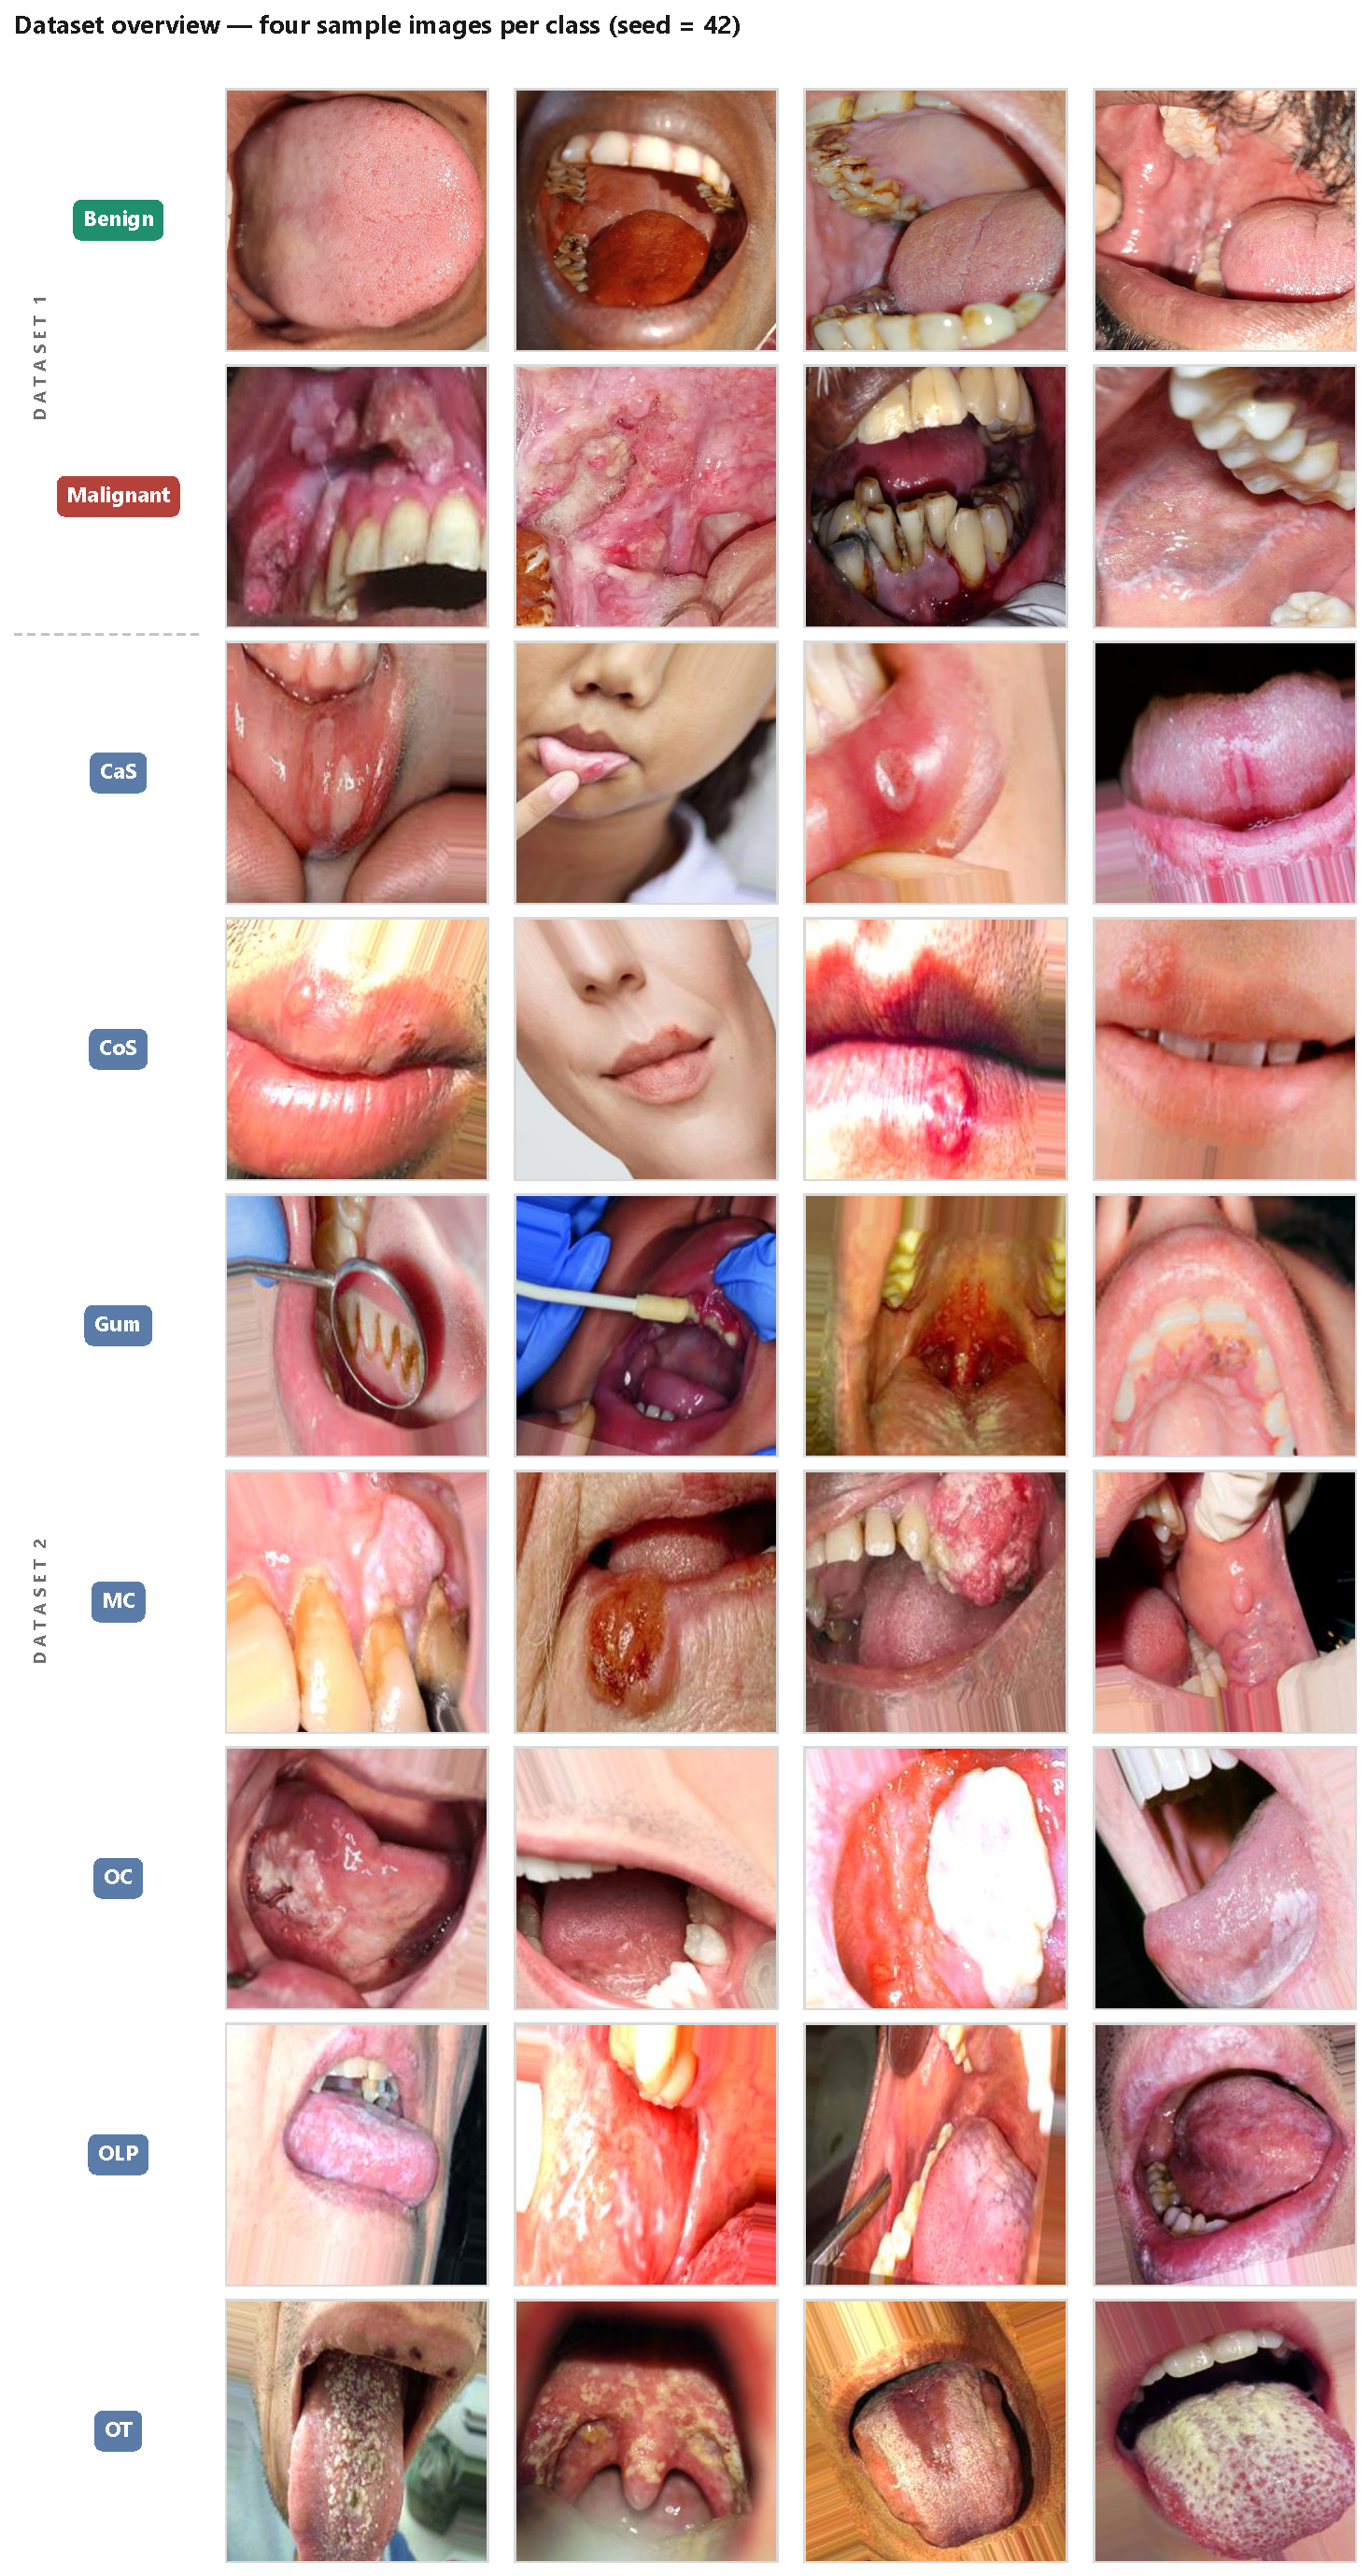
\includegraphics[width=\textwidth,height=0.92\textheight,%
  keepaspectratio]{fig02_dataset_sample_grid}
  \caption{Representative images from the two datasets, arranged as a
  9-row by 4-column grid: one class per row, with four randomly sampled
  examples per class shown across the four columns (seed${}={}$42). The top
  two rows show the DS1 binary categories (benign, malignant); the lower
  seven rows show the DS2 subtype classes CaS, CoS, Gum, MC, OC, OLP, and
  OT. Several subtypes share overlapping colour, texture, and boundary
  appearance, which is the visual difficulty that the seven-class head must
  resolve.}
  \label{fig:dataset}
\end{figure*}

\begin{figure}[!t]
  \centering
  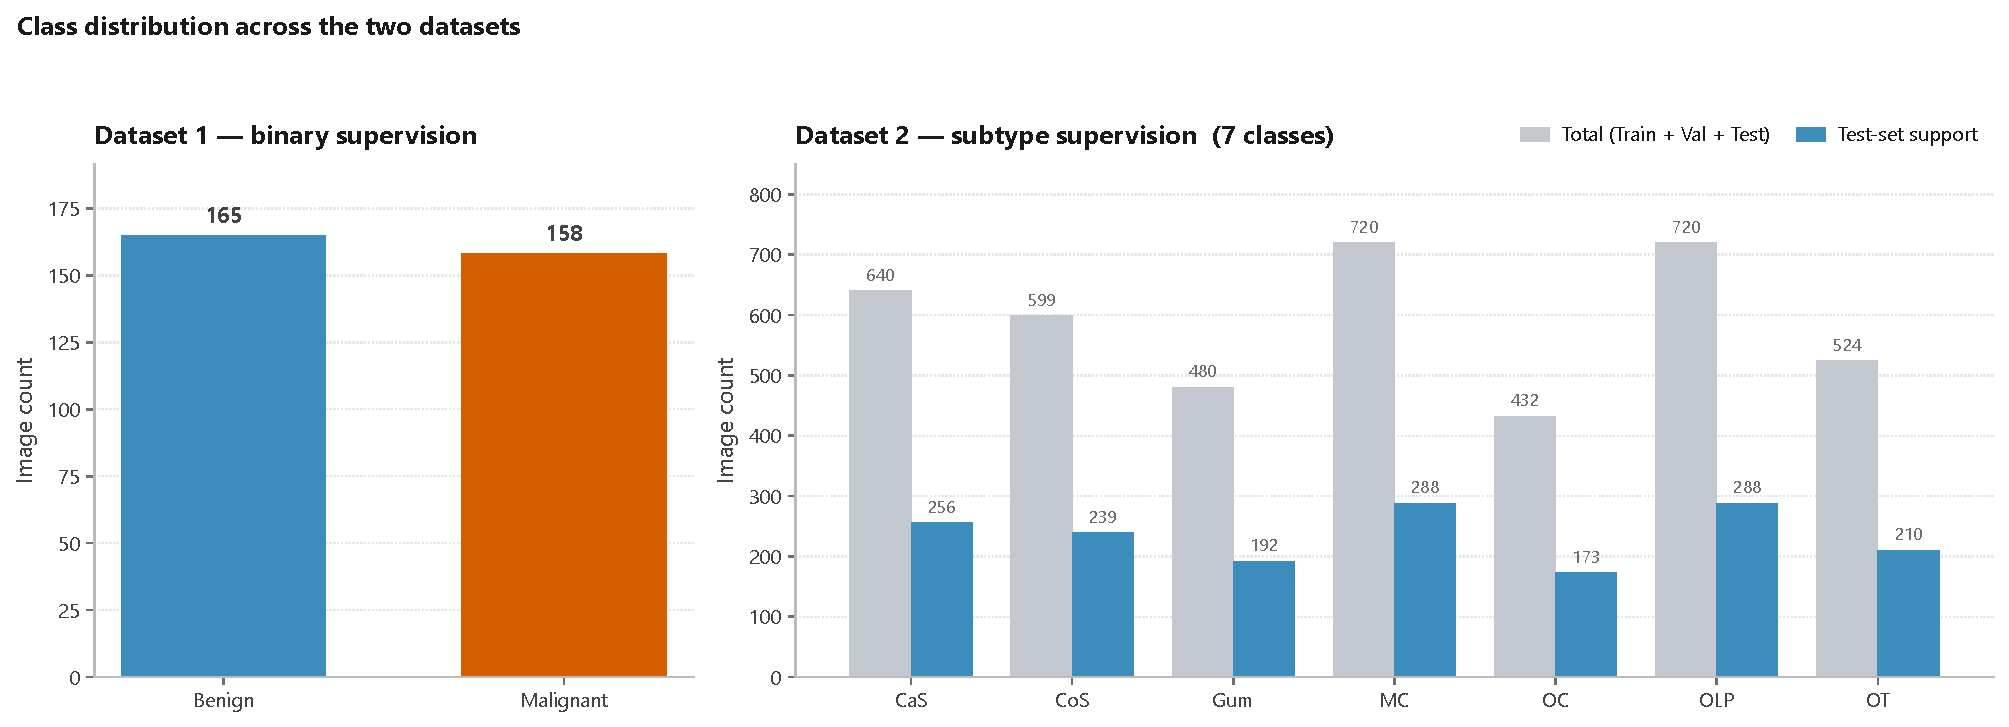
\includegraphics[width=\columnwidth]{fig02b_class_distribution}
  \caption{Class distribution across the two datasets. \emph{Left:} DS1
  benign-versus-malignant image counts. \emph{Right:} for each DS2 subtype,
  the total number of images across the merged train, validation, and test
  partitions, alongside the held-out test-set support used for per-class
  reporting in Section~\ref{sec:results}.}
  \label{fig:classdist}
\end{figure}

\subsection{Dual-Head Multi-Task Classifier}\label{ssec:dualhead}

All ten architectures evaluated in this study (nine baseline backbones
and the proposed model) share a common dual-head wrapper, denoted
\texttt{MultiTaskOralClassifier}. A shared backbone produces a pooled
feature vector, after which two independent multilayer perceptron (MLP)
heads predict the binary class (2 logits) and the subtype class (7 logits).
Each head is a \texttt{Linear}$(F\!\rightarrow\!512)\rightarrow
\text{ReLU}\rightarrow\text{Dropout}\rightarrow
\texttt{Linear}(512\!\rightarrow\!C)$ stack, where $F$ is the
backbone feature dimensionality and $C$ is the head's class count. A shared
dropout layer with rate $p=0.5$ is applied to the pooled features before
either head, providing the principal regularisation against over-fitting on
a dataset of modest scale.

The dual-head construction is what allows DS1, which carries only binary
labels, and DS2, which carries both binary and subtype labels, to train a
single model jointly: the subtype loss is masked for samples that lack a
subtype label, as detailed in Section~\ref{ssec:loss}. Sharing the backbone
across both tasks also forces the learned representation to be useful for
benign-versus-malignant screening and for fine-grained subtype
discrimination simultaneously, rather than specialising to either task in
isolation.

\subsection{Custom EfficientNet V2 Backbone}\label{ssec:backbone}

The proposed backbone is a five-stage CNN derived from the
\texttt{tf\_efficientnetv2\_b0} reference, the smallest member of the
EfficientNetV2 family~\cite{tan2021effv2}. Two structural
changes are applied to the donor architecture, and only these two; every
other stage is retained verbatim from the EfficientNetV2-B0 reference so
that the contribution of each change can be measured cleanly.

\begin{enumerate}
  \item \textbf{Stage-4 replacement.} The donor's Block-4, a Mobile
  Inverted Bottleneck Convolution (MBConv) block fused with a
  Squeeze-and-Excitation (SE) unit mapping $96 \rightarrow 112$ channels,
  is removed and replaced by an \emph{AttentionHub}
  (Section~\ref{ssec:hub}) with identical input and output channel counts.
  The hub is the only stage whose internal structure departs from the
  EfficientNetV2-B0 reference, and it is the only component the ablation of
  Section~\ref{sec:ablation} varies.
  \item \textbf{Tail trimming.} The donor's Block-6 and its
  \texttt{conv\_head} are dropped as redundant for this task. The
  192-channel output of Stage~5 is pooled directly into the dual-head
  classifier, which removes a substantial parameter and compute cost
  carried by the donor's wide convolutional head.
\end{enumerate}

The resulting backbone comprises five stages: \emph{Stem${}+{}$Block-0
${}+{}$Block-1} (32 channels) $\rightarrow$ \emph{Block-2} (48)
$\rightarrow$ \emph{Block-3} (96) $\rightarrow$ \emph{AttentionHub} (112)
$\rightarrow$ \emph{Block-5} (192), followed by global average pooling
and the two heads. The complete model contains between 4.79~M and 4.80~M
parameters and requires between 0.493 and 0.495 GFLOPs across the
attention-bearing ablation variants reported in Section~\ref{sec:ablation};
the no-attention control, which restores the donor's heavier
MBConv${}+{}$SE Block-4, is the exception at 5.70~M parameters and 0.636
GFLOPs (Table~\ref{tab:ablation}). The proposed configuration sits at the
lower end of the attention-bearing range (4.79~M parameters, 0.493 GFLOPs).
The full backbone, the Stage-4 hub, the global average pooling stage, and
the dual-head split are diagrammed in Fig.~\ref{fig:arch}.

\begin{figure*}[!t]
  \centering
  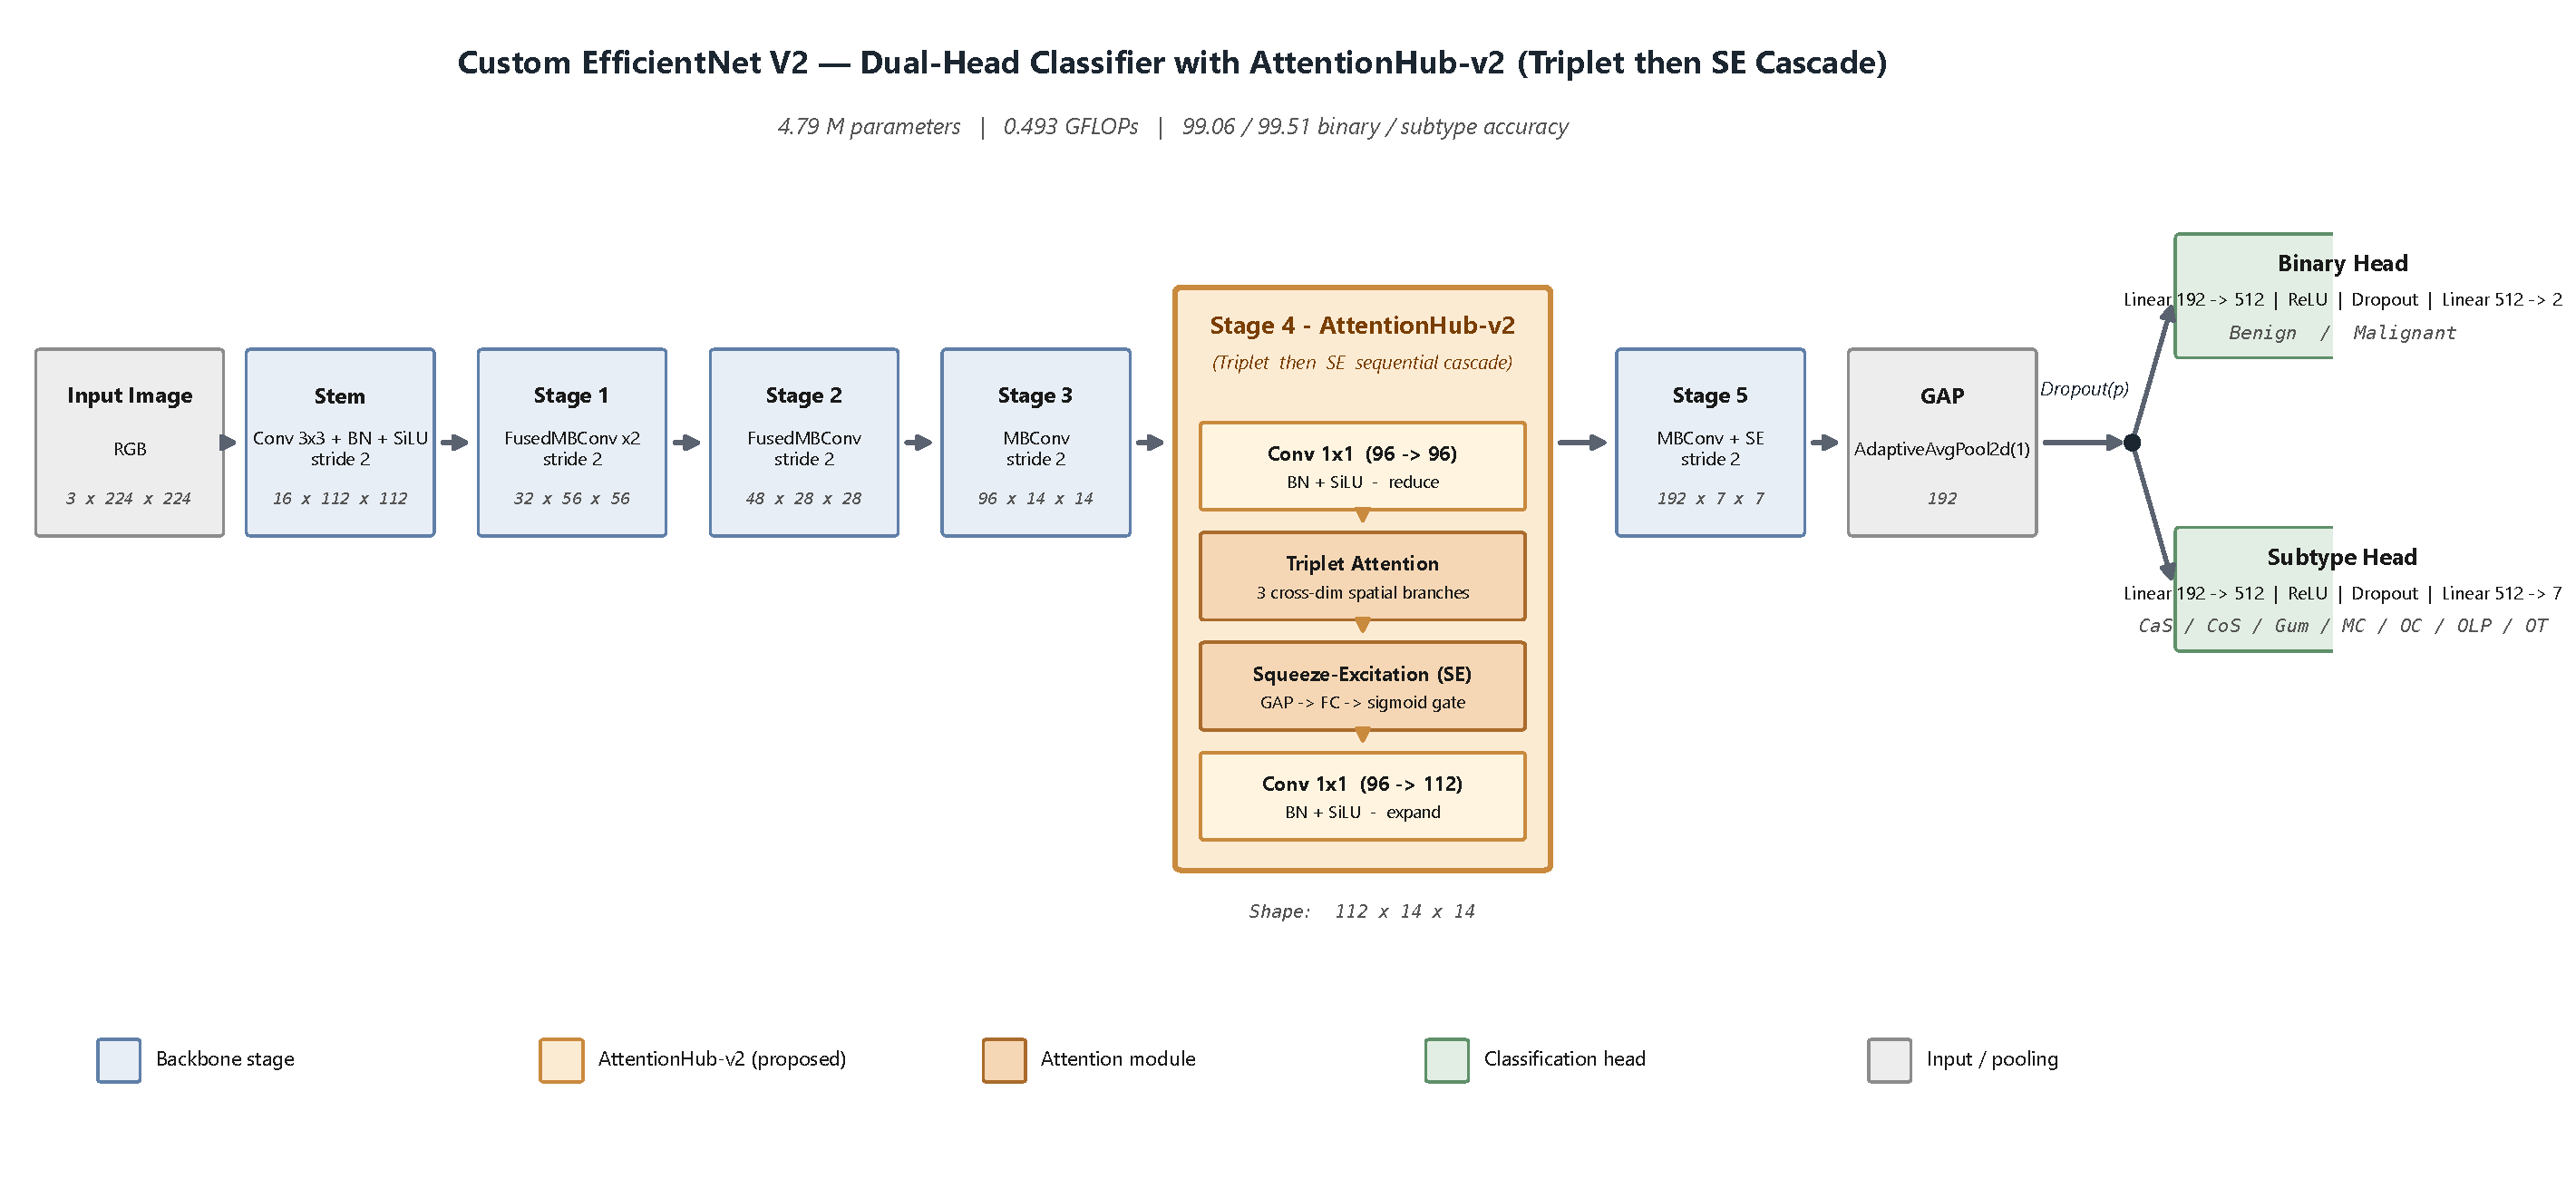
\includegraphics[width=\textwidth]{fig01_custom_efficientnet_v2_arch}
  \caption{The proposed Custom EfficientNet V2. A five-stage backbone
  derived from EfficientNetV2-B0 feeds a global average pooling layer and a
  shared dropout, after which two independent MLP heads predict the binary
  (benign / malignant) and subtype (7-class) labels. Stage~4 is replaced by
  the proposed AttentionHub-v2, a sequential Triplet$\rightarrow$SE cascade
  flanked by $1\times1$ channel-reduction and channel-expansion
  projections; the donor's Block-6 and convolutional head are removed. The
  complete model has 4.79~M parameters and 0.493 GFLOPs.}
  \label{fig:arch}
\end{figure*}

\subsection{AttentionHub Variants}\label{ssec:hub}

The AttentionHub is the single module whose composition changes across
ablation cells and across the two versions of the design presented here.
Both versions occupy Stage~4 of the backbone and preserve the
$96 \rightarrow 112$ channel mapping of the block they replace.

\paragraph{AttentionHub-v1 (parallel triple)}
The originally proposed hub routes the Stage-3 output through three parallel
attention branches: Bottleneck Attention Module (BAM), Triplet Attention,
and Kolmogorov--Arnold Network attention (KAN-Attention). Each branch is preceded
by a $1\times1$ channel-reduction projection that halves the branch channel
count. The three branch outputs are concatenated and fused by a $1\times1$
projection back to 112 channels. Ablation of v1 is implemented by removing
branches: the empty configuration restores the donor's original Block-4
(the canonical no-attention control), and any subset of
$\{\text{BAM},\text{Triplet},\text{KAN}\}$ is admissible. The three
candidate modules, whose internal structure is shown in
Fig.~\ref{fig:modules}, are as follows.

\begin{itemize}
  \item \textbf{BAM}~\cite{park2018bam} combines a channel gate (global
  average pooling followed by an MLP bottleneck) and a spatial gate
  ($1\times1 \rightarrow$ dilated $3\times3 \rightarrow 1\times1$, producing
  a single-channel spatial map). The two gates are summed, passed through a
  sigmoid, and multiplied with the input. BAM therefore exercises
  \emph{both} a channel and a spatial role.
  \item \textbf{Triplet Attention}~\cite{misra2021triplet} uses three
  branches, each applying a $7\times7$ attention gate to a permutation of
  the input tensor: the first branch swaps the channel and height axes, the
  second swaps the channel and width axes, and the third leaves the input
  in its native $(B,C,H,W)$ layout. Each gate applies a Z-Pool, which
  concatenates max- and mean-pooled statistics across the gated axis into
  two channels, followed by a $7\times7$ convolution and a sigmoid. The
  three branch outputs are averaged. Triplet exercises a
  \emph{cross-dimensional spatial} role at near-zero additional parameter
  cost.
  \item \textbf{KAN-Attention} is a Kolmogorov--Arnold-Network-inspired
  channel recalibration~\cite{liu2024kan}. Global average pooling produces
  a per-channel scalar; each scalar is passed through a learnable B-spline
  basis expansion (five Gaussian basis functions on $[-3,+3]$) with a SiLU
  residual, then sigmoid-gated and multiplied with the input. KAN-Attention
  is \emph{purely channel-wise} and supplies a non-linear alternative to the
  linear MLP used in the SE and BAM channel gates.
\end{itemize}

\paragraph{AttentionHub-v2 (sequential Triplet$\rightarrow$SE)}
The proposed model uses a sequential cascade in which the channel-reduced
feature is first refined by Triplet Attention and then by
Squeeze-and-Excitation (SE)~\cite{hu2018se}. The SE module pools globally,
passes the pooled descriptor through a two-layer $1\times1$ bottleneck with
reduction ratio 16 and a sigmoid gate, and multiplies the result back into
the input. No LayerScale, no per-module residual, and no additional gating
are introduced: both attentions are multiplicative gates that preserve the
input information without an explicit skip connection. The composition
order, spatial attention before channel attention, follows the
convention established by the Convolutional Block Attention Module
(CBAM)~\cite{woo2018cbam}. The internal layout of the v2 hub is shown in
Fig.~\ref{fig:hubv2}, and a side-by-side contrast with the v1 parallel hub
is given in Fig.~\ref{fig:v1v2}. The design rationale for v2 (in
particular, why a sequential cascade is preferred over the v1 parallel
fusion and why SE is chosen as the channel partner) is not asserted here
but \emph{derived} in Section~\ref{sec:ablation} from the v1 ablation.

\begin{figure*}[!t]
  \centering
  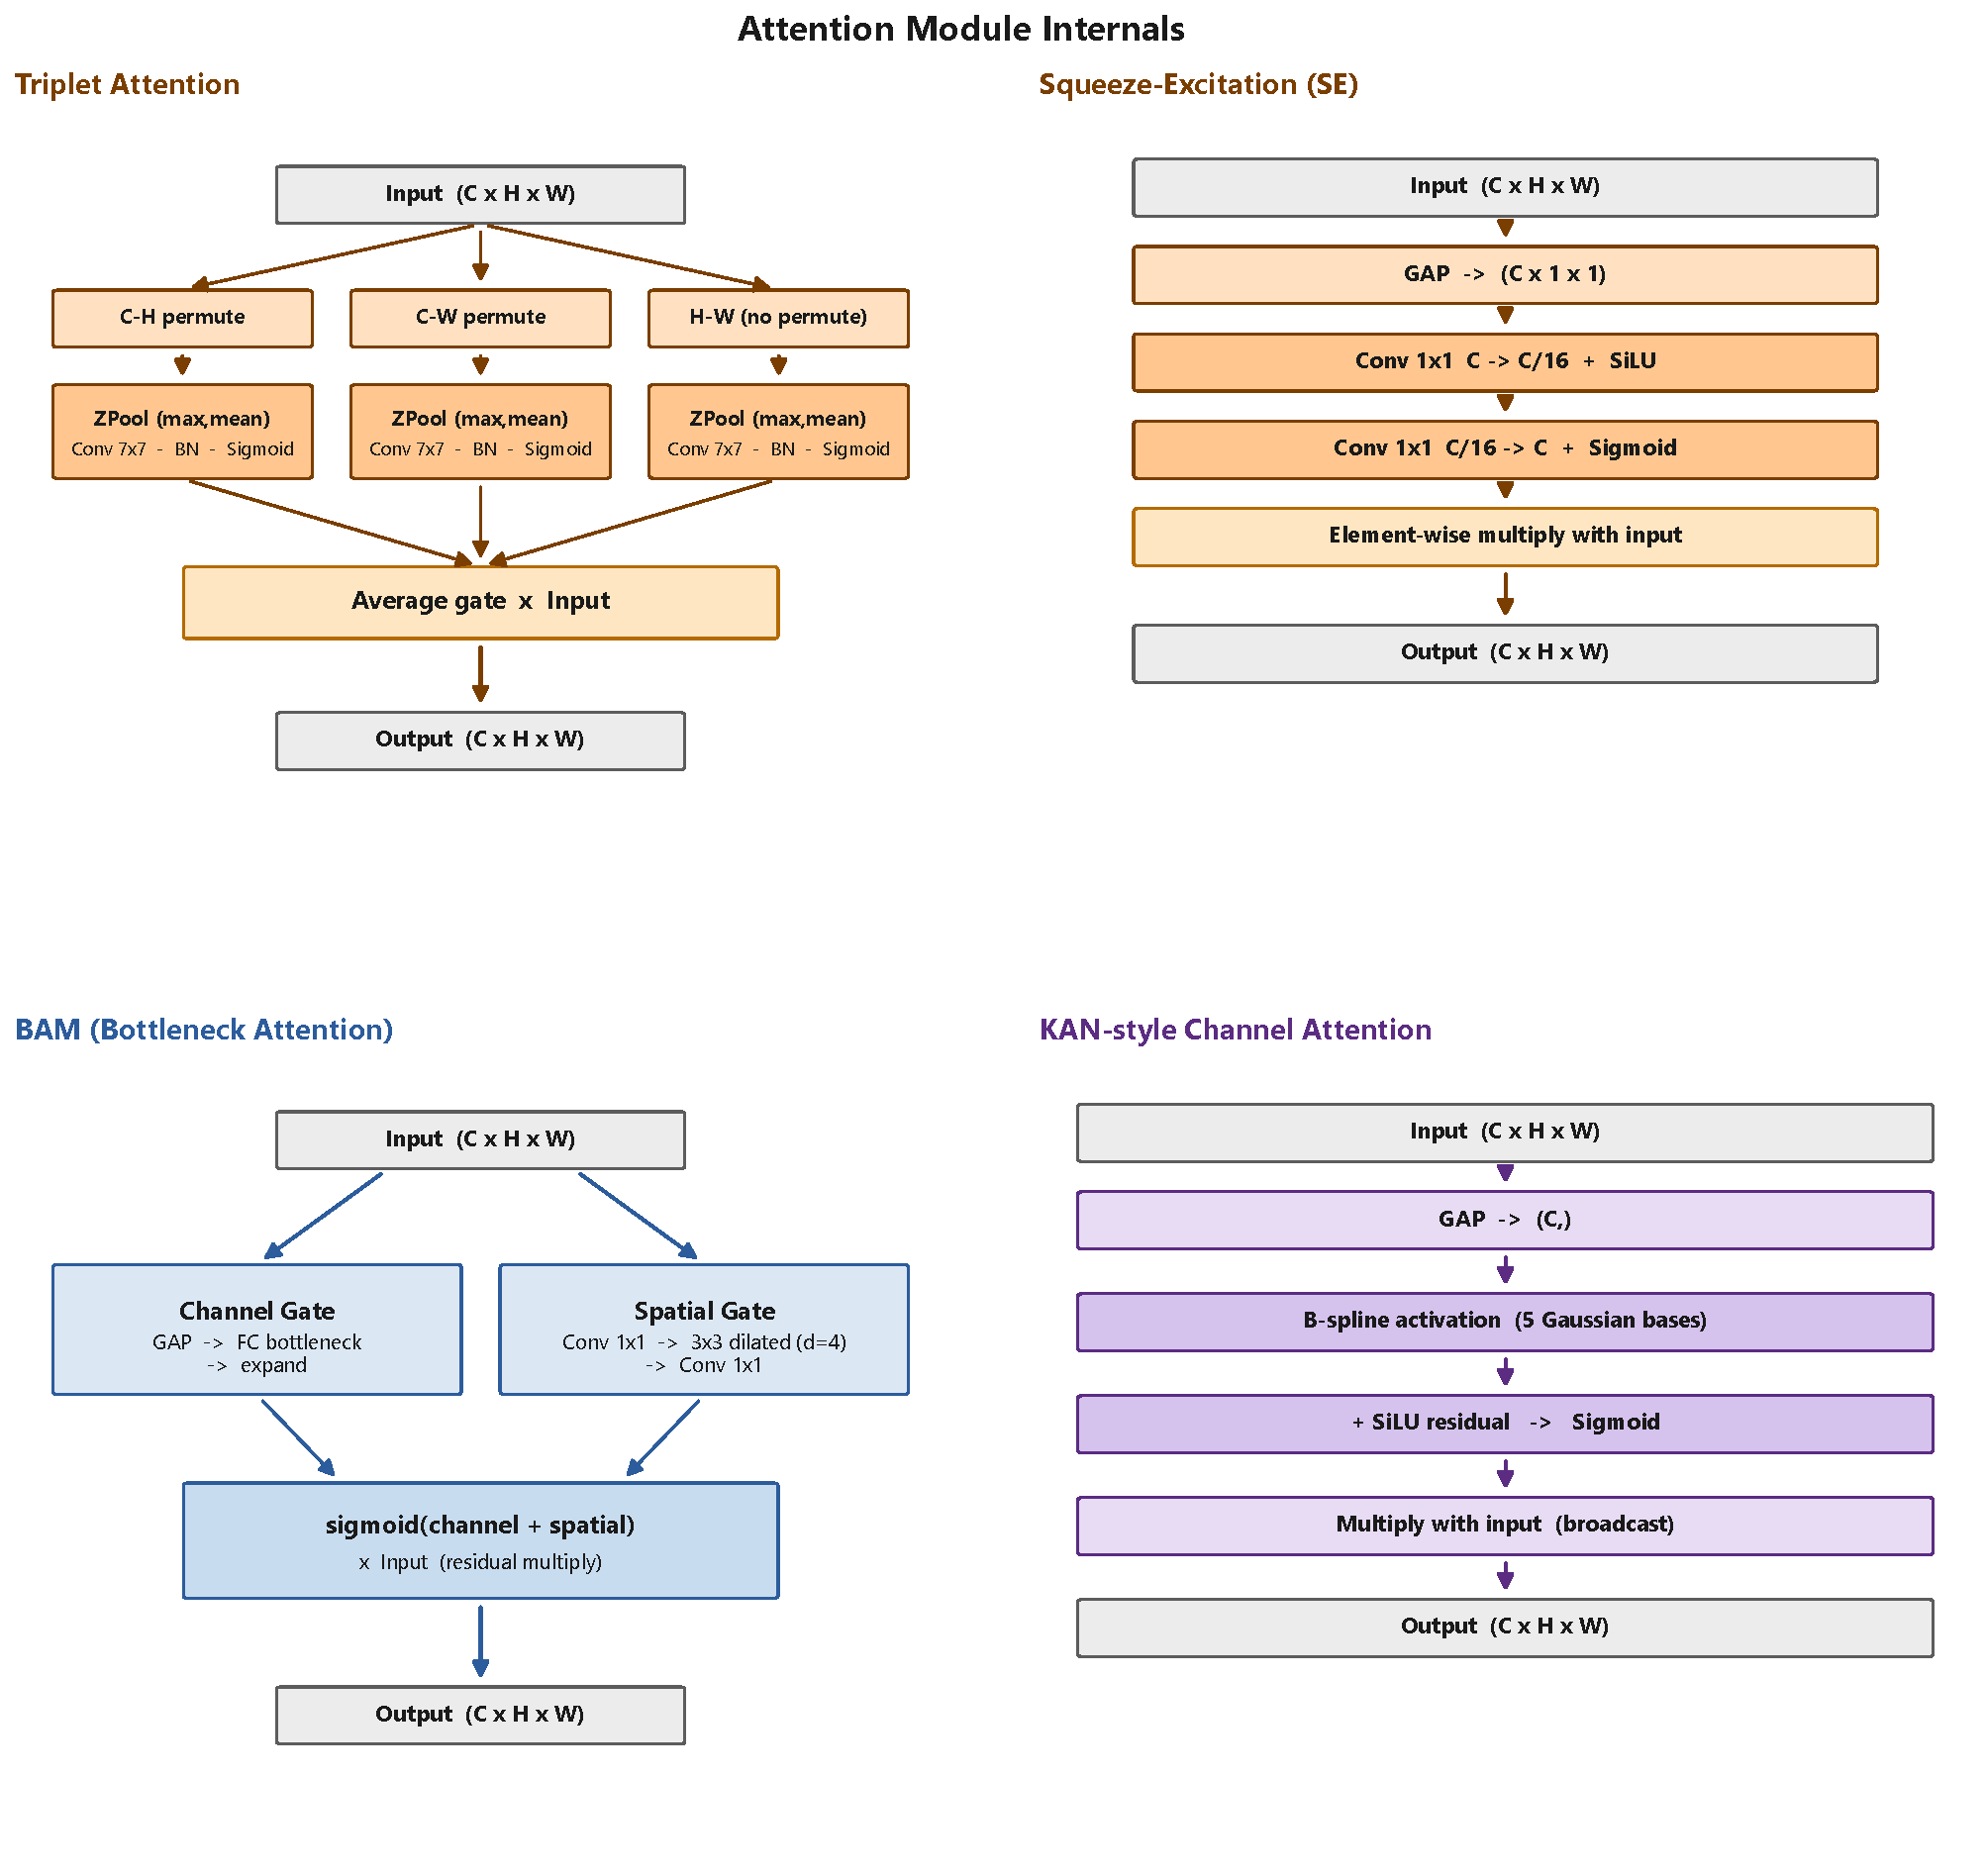
\includegraphics[width=\textwidth]{fig01d_attention_modules_internals}
  \caption{Internal structure of the four attention modules used in this
  study. \emph{Triplet Attention} applies a $7\times7$ gate to three
  axis-permuted views of the feature map and averages them, exercising a
  cross-dimensional spatial role. \emph{Squeeze-and-Excitation (SE)}
  recalibrates channels through a global-average-pooling bottleneck.
  \emph{BAM} sums a channel gate and a spatial gate, exercising a mixed
  role. \emph{KAN-Attention} replaces the linear channel MLP with a
  learnable B-spline basis expansion, remaining purely channel-wise.}
  \label{fig:modules}
\end{figure*}

\begin{figure}[!t]
  \centering
  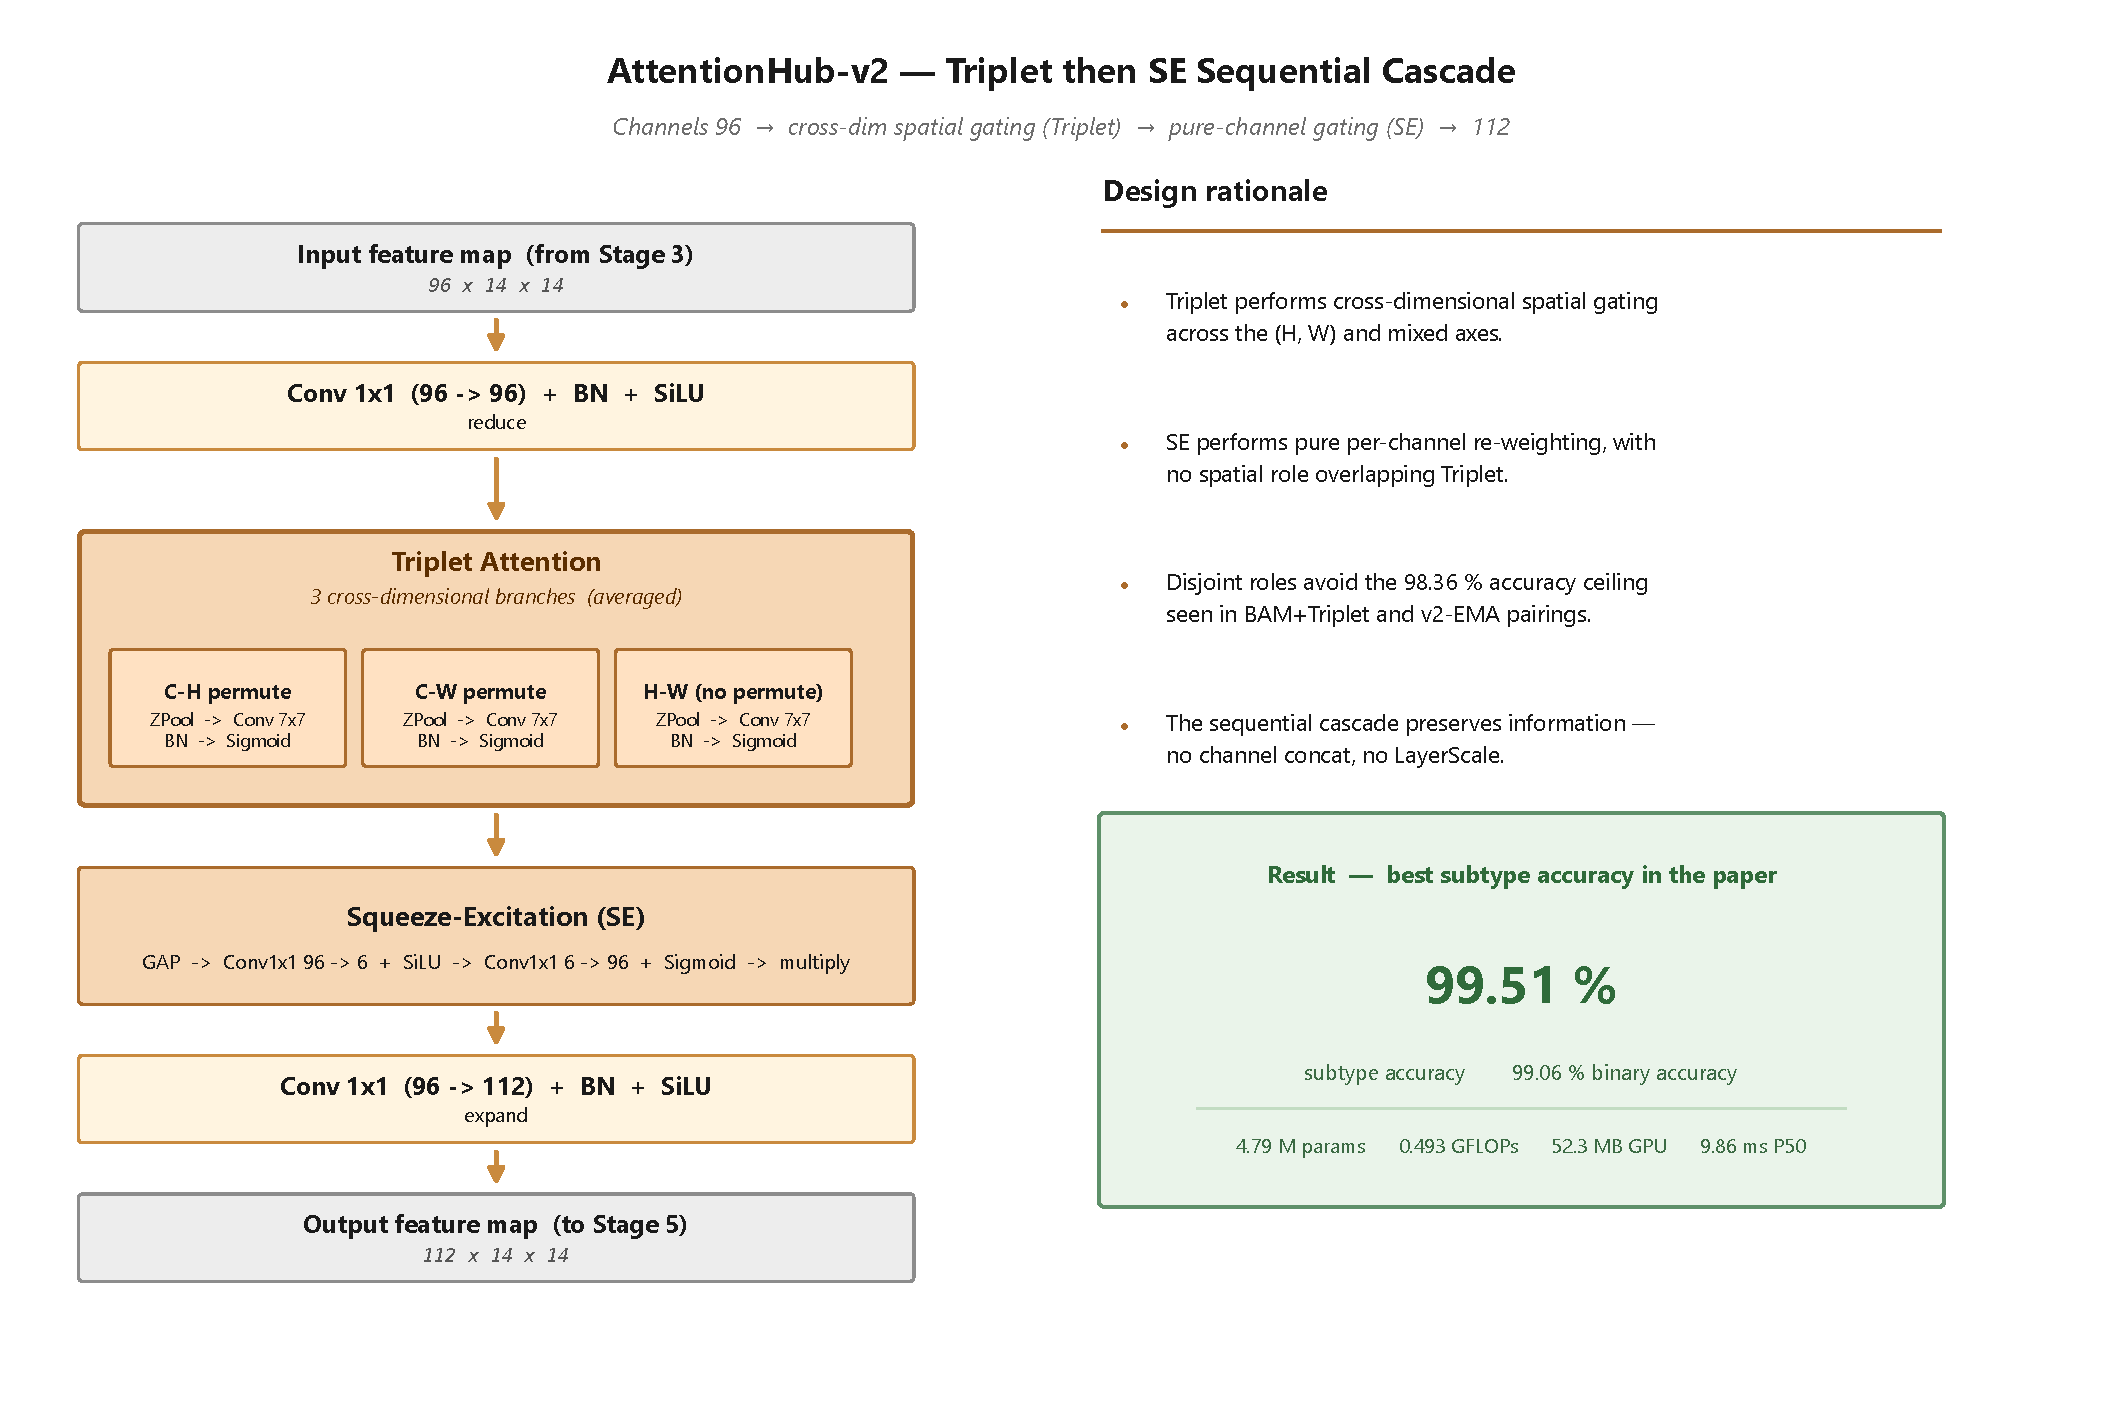
\includegraphics[width=\columnwidth]{fig01b_attentionhub_v2_detail}
  \caption{The proposed AttentionHub-v2. A $1\times1$ projection reduces the
  96-channel Stage-3 feature; Triplet Attention then applies
  cross-dimensional spatial gating, SE applies pure per-channel
  recalibration, and a $1\times1$ projection expands the result to 112
  channels for Stage~5. The two attention modules occupy disjoint functional
  roles (spatial and channel), which Section~\ref{sec:ablation} shows is
  the condition required to avoid the observed sub-baseline accuracy
  ceiling.}
  \label{fig:hubv2}
\end{figure}

\begin{figure*}[!t]
  \centering
  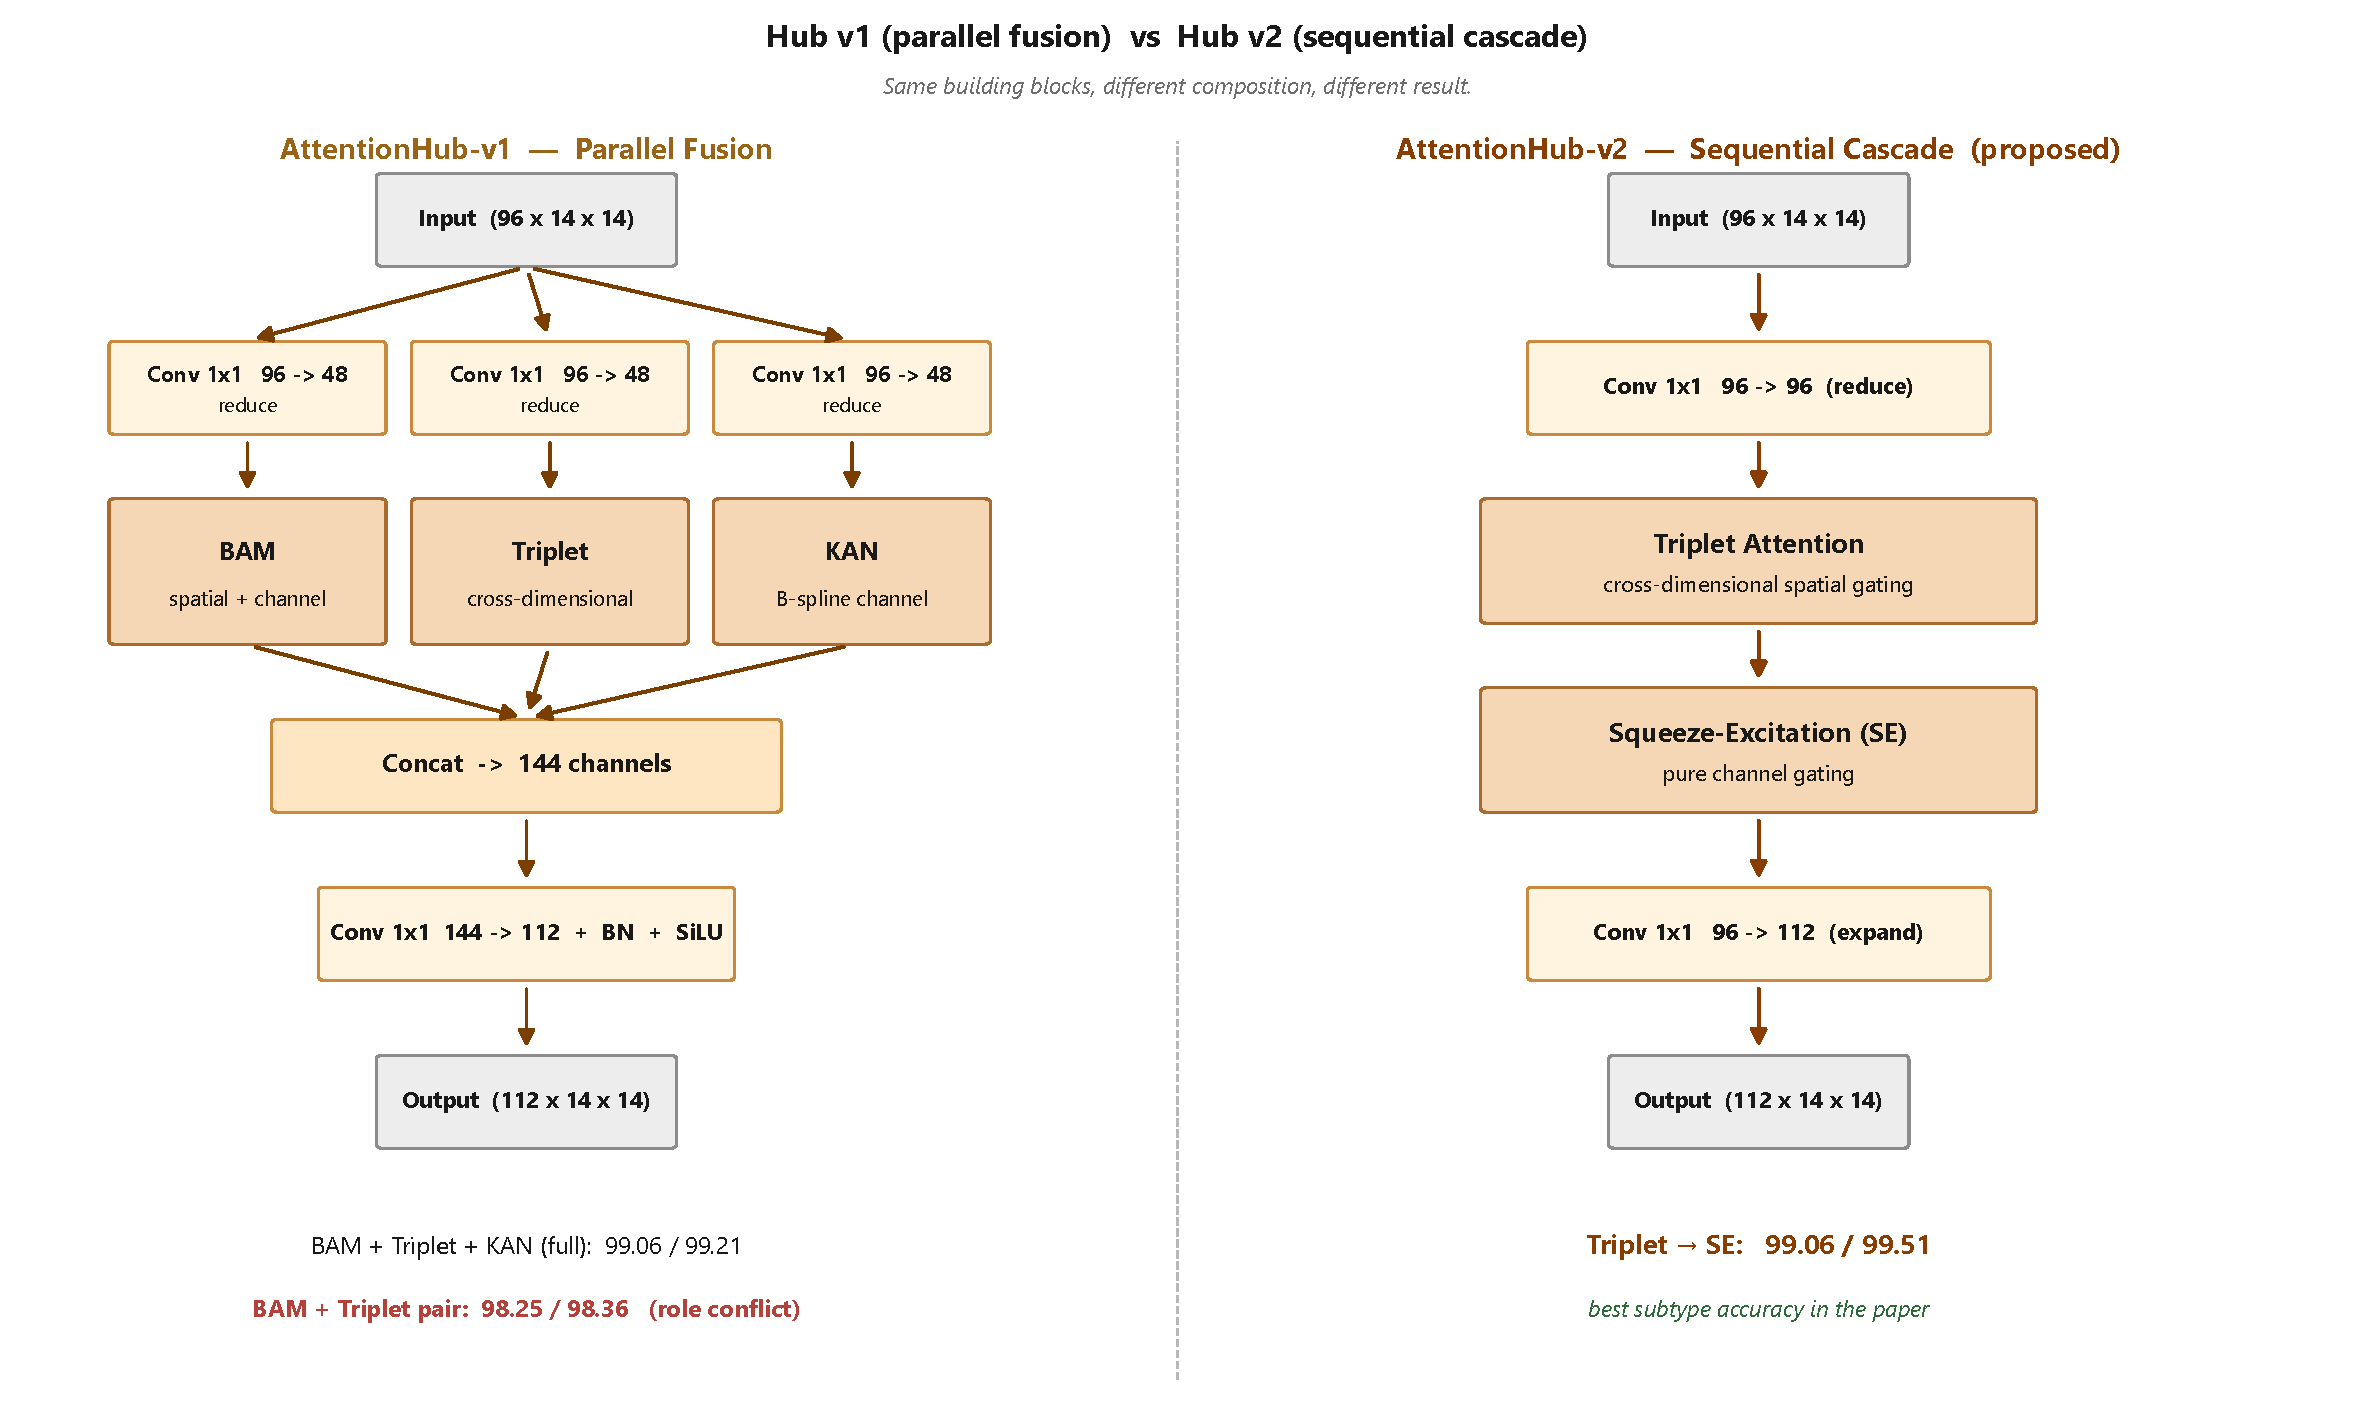
\includegraphics[width=\textwidth]{fig01c_attentionhub_v1_vs_v2}
  \caption{AttentionHub-v1 versus AttentionHub-v2. \emph{Left:} the v1 hub
  fuses BAM, Triplet, and KAN-Attention in parallel, concatenating their
  channel-reduced branch outputs before a $1\times1$ projection.
  \emph{Right:} the proposed v2 hub composes Triplet Attention and SE
  sequentially. The two hubs reuse the same building blocks but differ in
  composition; Section~\ref{sec:ablation} shows that the difference in
  composition is what separates their accuracy.}
  \label{fig:v1v2}
\end{figure*}

\subsection{Multi-Task Loss}\label{ssec:loss}

The two heads are trained jointly under a single combined cross-entropy
(CE) objective,

\begin{equation}\label{eq:loss}
  \begin{split}
  \mathcal{L} \;=\;{}& w_b \cdot \mathrm{CE}\!\left(p_{\text{binary}},\,
  y_{\text{binary}}\right) \\
  &{}+\; w_s \cdot \mathrm{CE}\!\left(
  p_{\text{subtype}},\, y_{\text{subtype}};\,
  \texttt{ignore\_index}=-1\right),
  \end{split}
\end{equation}

with equal task weights $w_b = w_s = 1$. The \texttt{ignore\_index}${}={}-1$
convention is the mechanism that lets the two datasets co-train against one
model: DS1 samples, which carry no subtype label, are assigned the sentinel
subtype label $-1$ and therefore contribute only to the binary term, while
DS2 samples contribute to both terms. A numerical guard converts any
not-a-number (NaN) subtype loss to zero, so that a mini-batch composed
exclusively of DS1 samples, for which the subtype term is undefined,
remains a valid training step.

The joint update is summarised in Algorithm~1, typeset in
Fig.~\ref{alg:train}. The masked subtype loss is the only coupling between
the binary-only DS1 and the dually labelled DS2: DS1 samples shape the
shared backbone solely through $\mathcal{L}_b$, whereas DS2 samples shape it
through both $\mathcal{L}_b$ and $\mathcal{L}_s$.

\begin{figure}[!t]
  \centering
  \fbox{%
  \begin{minipage}{0.92\columnwidth}
  \ttfamily \footnotesize
  \textbf{Algorithm 1:} Joint masked multi-task training step.\\[2pt]
  \textbf{Input:} mini-batch $(x, y_b, y_s)$; model $M = $ backbone\\
  \hphantom{\textbf{Input:} }${}+ (g_{\text{binary}}, g_{\text{subtype}})$;
  optimizer Opt;\\
  \hphantom{\textbf{Input:} }loss weights $(w_b, w_s)$.\\
  \textbf{Output:} updated model parameters.\\[3pt]
  1.\ \ $F \leftarrow$ backbone$(x)$ \hfill \# $B \times D$\\
  2.\ \ $F \leftarrow$ Dropout$(F,\ p = 0.5)$\\
  3.\ \ $\hat{y}_b \leftarrow g_{\text{binary}}(F)$ \hfill \# $B \times 2$\\
  4.\ \ $\hat{y}_s \leftarrow g_{\text{subtype}}(F)$ \hfill \# $B \times 7$\\
  5.\ \ $L_b \leftarrow$ CE$(\hat{y}_b,\ y_b)$ \hfill \# always defined\\
  6.\ \ $L_s \leftarrow$ CE$(\hat{y}_s,\ y_s;$ ignore\_index $= -1)$\\
  \hphantom{6.\ \ }\hfill \# NaN if every $y_s = -1$\\
  7.\ \ \textbf{if} isnan$(L_s)$\textbf{:}\ \ $L_s \leftarrow 0$
  \hfill \# DS1-only batch guard\\
  8.\ \ $L_{\text{total}} \leftarrow w_b \cdot L_b + w_s \cdot L_s$\\
  9.\ \ Opt.zero\_grad()\textbf{;}\ \ $L_{\text{total}}$.backward()%
  \textbf{;}\ \ Opt.step()
  \end{minipage}}
  \caption{Joint training step under the masked multi-task loss. The
  sentinel subtype label $-1$ marks DS1 (binary-only) samples; the
  \texttt{ignore\_index} convention and the NaN guard on line~7 together
  allow DS1 and DS2 to co-train a single shared backbone.}
  \label{alg:train}
\end{figure}

\subsection{Training Protocol}\label{ssec:training}

All ten models (the nine baseline backbones and the proposed model)
are trained from scratch under a single matched recipe, deliberately chosen
to guarantee a fair comparison. \textbf{No ImageNet pre-trained weights are
used.} Pre-training would smuggle a representational prior into the
comparison and confound the contribution of the dataset itself with the
contribution of the architecture; training every model from random
initialisation removes that confound and isolates what each backbone learns
from the oral-disease data alone. The recipe is fixed as follows.

\begin{itemize}
  \item \textbf{Optimiser:} Adam~\cite{kingma2015adam}, learning rate
  $1\times10^{-4}$, weight decay $1\times10^{-4}$.
  \item \textbf{Scheduler:} cosine annealing over the full epoch budget.
  \item \textbf{Batch size:} 64, with gradient accumulation factor 1
  (effective batch size 64).
  \item \textbf{Epoch budget:} 200, with early stopping (patience 15,
  minimum improvement $\Delta = 1\times10^{-4}$ on validation loss).
  \item \textbf{Seed:} 42, with deterministic CuDNN.
  \item \textbf{Image size:} $224\times224$.
  \item \textbf{Hardware:} a single NVIDIA GeForce RTX~4060~Ti.
\end{itemize}

This recipe is enforced for every model without exception. In particular,
the AttentionHub ablation variants are forced onto the identical baseline
recipe, so that v1, v2, and the seven ablation cells of
Section~\ref{sec:ablation} are directly comparable. Per-model
hyper-parameter tuning is deliberately \emph{not} performed: tuning would
advantage the models we elect to tune and disadvantage those we do not,
reintroducing exactly the kind of uncontrolled variable that a fair
benchmark must eliminate. Where a baseline encounters memory pressure on the
16~GB GPU, the correct response under this protocol is gradient
accumulation at a fixed effective batch size, not a per-model
hyper-parameter override, a stance established by prior fair-comparison
work and retained here as a methodological commitment rather than a
convenience.

\subsection{Evaluation Protocol}\label{ssec:evaluation}

For every model we report the following quantities on the held-out test
set.

\begin{itemize}
  \item \textbf{Classification metrics:} accuracy, weighted precision,
  weighted recall, and weighted F1, for both the binary head (the DS1 test
  split together with the full DS2 test set, $1\,711$ images in total) and the
  subtype head (the DS2 seven-class test set, $1\,646$ images).
  \item \textbf{Per-class report:} precision, recall, F1, and support for
  each of the seven subtype classes.
  \item \textbf{Confusion matrices:} the binary and subtype confusion
  matrices, reported side by side.
  \item \textbf{Computational metrics:} parameter count, GFLOPs computed
  with \texttt{thop}, on-disk model size in megabytes, GPU peak memory
  during inference,\footnote{Compute is reported as the multiply-accumulate
  (MAC) count returned by the \texttt{thop} profiler, following common
  practice; we use the label GFLOPs for these MAC-count values for
  consistency with the comparison literature.} the mean and standard
  deviation of single-image
  inference latency (a 200-iteration warm-up followed by 1\,000 timed
  iterations), the P50 / P90 / P95 / P99 latency percentiles (of which
  the P50 and P95 values are tabulated in Section~\ref{sec:results}),
  energy in kWh and carbon in kg~CO\textsubscript{2}-equivalent measured
  with \texttt{codecarbon} where available, total training time, and the
  number of epochs completed before early stopping.
  \item \textbf{Explainability artifacts:} for each model, a
  Gradient-weighted Class Activation Mapping++ (Grad-CAM++) panel and a Local
  Interpretable Model-Agnostic Explanations (LIME) boundary-mask panel for
  the binary head, and the matching pair for the subtype head, evaluated on
  a class-balanced sample of test images.
\end{itemize}

The per-model JSON metric files, training-time logs, latency histograms,
confusion matrices, and explainability images are released alongside the
paper so that every reported number can be independently regenerated.

\subsection{Ablation Protocol}\label{ssec:ablation_protocol}

The AttentionHub-v1 ablation is implemented as a code-level branch switch:
each ablation key maps to a tuple of active branches, a subset of
$\{\text{bam},\text{triplet},\text{kan}\}$, where the empty tuple falls
back to the donor's original Block-4 and thus serves as the no-attention
control. Because the switch operates inside the hub and changes nothing
else in the network or the recipe, the eight cells differ from one another
only in which attention branches are active, the property required for
the ablation to be causally interpretable. The eight cells are listed in
Table~\ref{tab:ablkeys}, together with the functional role each
configuration's hub exercises.

\begin{table}[!t]
  \centering
  \caption{AttentionHub-v1 ablation keys. Each key activates a subset of the
  three candidate branches; the empty configuration restores the donor
  MBConv${}+{}$SE Block-4 as the no-attention control. The role column
  classifies the configuration by the functional role its hub exercises and
  is the basis of the role-complementarity analysis in
  Section~\ref{sec:ablation}.}
  \label{tab:ablkeys}
  \begin{tabularx}{\columnwidth}{@{}l l X@{}}
    \hline
    Key & Active branches & Functional role \\
    \hline
    \texttt{none} & --- (donor MBConv${}+{}$SE) & no-attention control \\
    \texttt{bam} & BAM & spatial${}+{}$channel singleton \\
    \texttt{triplet} & Triplet & cross-dim-spatial singleton \\
    \texttt{kan} & KAN & channel singleton \\
    \texttt{bam\_triplet} & BAM${}+{}$Triplet & two-spatial-role pair \\
    \texttt{bam\_kan} & BAM${}+{}$KAN & mixed-role pair \\
    \texttt{triplet\_kan} & Triplet${}+{}$KAN &
      cross-dim-spatial${}+{}$pure-channel pair \\
    \texttt{full} (${}={}$v1) & BAM${}+{}$Triplet${}+{}$KAN &
      original proposed model \\
    \hline
  \end{tabularx}
\end{table}

In addition, we report a v2-EMA run, a sequential Triplet${}+{}$Efficient
Multi-scale Attention (EMA) cascade, which is \emph{not} an ablation cell
but a deliberate stress test of the role-complementarity principle: it
replaces SE with EMA, a module that combines a multi-scale spatial branch
with a channel branch. Because EMA exercises a spatial role, the principle
predicts that the v2-EMA cascade should regress, and the result reported in
Section~\ref{sec:ablation} confirms this prediction. Every ablation cell is
trained under the identical baseline recipe used by the nine baseline
backbones; no recipe exceptions apply.

\section{Experimental Setup}\label{sec:setup}

This section records the hardware and software environment in which every
experiment was executed, the provisions made to keep the study
reproducible, and the ethical considerations that bound its scope.

\subsection{Hardware and Software Stack}\label{ssec:hardware}

All experiments are executed on a single workstation equipped with an
\textbf{NVIDIA GeForce RTX~4060~Ti} graphics processing unit (16~GB GDDR6),
32~GB of system memory, and an AMD Ryzen~7 central processing unit. Using a
single fixed machine for every run keeps the measured latency, GPU peak
memory, training time, and energy figures mutually comparable, since they
are not contaminated by hardware variation across models. The exact Ryzen~7
SKU was not recorded; this does not affect the latency and GPU-memory
figures, which are GPU-bound and CPU-insensitive, but it is relevant to the
wall-clock training time of Table~3, the one CPU-sensitive measurement, and
that table is therefore reported with the explicit caveat given in
Section~\ref{sec:results} that wall-clock training time is not controlled
across runs.

The software stack is held fixed across all runs: Python~3.11 and
PyTorch~2.x with CUDA~12; \texttt{timm}~0.9 for the structural definition of
the donor EfficientNetV2-B0 backbone, of which only the architectural reference
is used (the pre-trained weights are explicitly \emph{not} loaded, in
keeping with the from-scratch training protocol of
Section~\ref{ssec:training}); \texttt{thop} for floating-point operation
counting; \texttt{pytorch-grad-cam}~1.5 for the Grad-CAM++ saliency maps;
\texttt{lime}~0.2 together with \texttt{scikit-image} for the super-pixel
boundary masks; and \texttt{codecarbon} for energy and
CO\textsubscript{2}-equivalent emissions tracking. Deterministic CuDNN is
enabled for every reported run.

\subsection{Reproducibility Provisions}\label{ssec:reproducibility}

The complete experimental package is structured for reproducibility along
five axes.

\begin{enumerate}
  \item \textbf{Code and configuration release.} The full training,
  evaluation, and metric-computation scripts are provided in the
  repository. A single configuration file (\texttt{configs/config.py})
  controls every global hyper-parameter and is enforced across all runs, so
  that the matched recipe of Section~\ref{ssec:training} cannot drift
  between models.
  \item \textbf{Fixed seed.} Every run uses random seed 42 for Python,
  NumPy, and PyTorch, and CuDNN deterministic mode is enabled.
  \item \textbf{Fixed split.} The dataset splits are deterministic functions
  of the seed, which makes train/test contamination across runs impossible
  by construction.
  \item \textbf{Per-run JSON.} Every one of the ten models (the nine
  baseline backbones and the proposed model) emits a
  \texttt{classification\_metrics.json}, a \texttt{performance\_metrics%
  .json}, a \texttt{training\_time.json}, and a per-class textual report
  (\texttt{evaluation\_results.txt}); all of these are committed alongside
  the trained model weights, so that every classification and computational
  number reported in Section~\ref{sec:results} can be independently
  regenerated for both the baseline rows and the proposed model.
  \item \textbf{Explainability artifacts.} The Grad-CAM++ and LIME panels for
  both heads (\texttt{explain\_binary.png} and
  \texttt{explain\_subtype.png}) are produced by a single script
  (\texttt{explain\_model.py}) under identical preprocessing for every
  model.
\end{enumerate}

A small number of runs (the AttentionHub ablation cells) include
\texttt{codecarbon}-measured energy and CO\textsubscript{2} figures, whereas
the older baseline runs report the conservative analytical estimate used in
the absence of \texttt{codecarbon} at the time those runs were executed. We
retain both forms of the measurement, and label them as such, in the
interest of transparency.

\subsection{Ethical Considerations}\label{ssec:ethics}

The datasets used in this study are pre-existing curated collections of oral
lesion images. They are used solely for non-clinical research purposes, and
all results are reported on a held-out split that is disjoint from the
training and validation data. No patient-identifying information is present
in the datasets, and no human subjects are recruited as part of this work.

The proposed model is \emph{not} a clinical decision-support system and
should not be used as one without appropriate clinical validation,
regulatory clearance, and prospective evaluation. We further acknowledge
that automated screening systems can perpetuate disparities present in their
training data: in particular, the demographic composition and
intra-oral-anatomy coverage of the datasets are not characterised in their
published metadata, and external validation across diverse patient
populations is required before any clinical claim can be made. The model is
released under a research-use license, with the explicit intent of enabling
replication and methodological extension rather than direct clinical
deployment.

\section{Baseline Benchmark Results}\label{sec:results}

This section establishes the empirical reference frame against which the
proposed model is judged. Ten architectures --- the nine standard baselines and
the proposed Custom EfficientNet~V2 --- are trained from scratch under the
single matched recipe of Section~\ref{sec:methods}, with no per-model
hyper-parameter tuning, and evaluated once on the held-out test set. The
benchmark is reported along three axes: classification accuracy on both heads
(Section~\ref{subsec:quant}), per-class subtype behaviour
(Section~\ref{subsec:perclass}), and computational efficiency
(Section~\ref{subsec:efficiency}). The ablation that explains \emph{why} the
proposed hub is designed as it is follows in Section~\ref{sec:ablation}; the
present section is concerned only with where the proposed model sits relative
to the field.

\subsection{Quantitative Comparison}\label{subsec:quant}

Table~\ref{tab:benchmark} reports the held-out test performance of all ten
architectures on both the binary (benign versus malignant) and the seven-class
subtype head, alongside parameter count, compute cost in GFLOPs,
and on-disk model size. Every value derives from a single training run per
model under the matched recipe; no figure in the table benefits from per-model
tuning, so the comparison isolates architecture rather than optimisation
effort.

\begin{table*}[!t]
\caption{Test-set classification performance under the matched fair recipe.
All ten architectures are trained from scratch (no ImageNet pre-training) with
identical optimiser, schedule, batch size, and seed. Bold marks the
proposed-model row and the best value in each column.}
\label{tab:benchmark}
\centering
\resizebox{\textwidth}{!}{%
\begin{tabular}{l d{4} d{4} d{4} d{4} d{2} d{3} d{2}}
\hline
\multicolumn{1}{l}{Model} &
\multicolumn{1}{c}{Binary Acc} &
\multicolumn{1}{c}{Binary F1} &
\multicolumn{1}{c}{Subtype Acc} &
\multicolumn{1}{c}{Subtype F1} &
\multicolumn{1}{c}{Params (M)} &
\multicolumn{1}{c}{GFLOPs} &
\multicolumn{1}{c}{Size (MB)} \\
\hline
ResNet50            & 0.9912 & 0.9912 & 0.9909 & 0.9909 & 25.61 & 4.134 & 98.01 \\
DenseNet121         & 0.9889 & 0.9889 & 0.9933 & 0.9933 &  7.92 & 2.834 & 31.15 \\
ConvNeXt-Tiny       & 0.9532 & 0.9533 & 0.9046 & 0.9048 & 28.59 & 4.456 & 109.22 \\
Swin-T              & 0.9819 & 0.9819 & 0.9769 & 0.9769 & 28.29 & 4.372 & 108.07 \\
EfficientNet-B0     & 0.9883 & 0.9883 & 0.9903 & 0.9903 &  5.28 & 0.386 & 20.60 \\
EfficientNet V2-B2  & \multicolumn{1}{c}{\textbf{0.9936}} & \multicolumn{1}{c}{\textbf{0.9936}} & 0.9933 & 0.9933 & 10.00 & 1.100 & 39.17 \\
EfficientNet V2-B3  & 0.9889 & 0.9889 & 0.9842 & 0.9842 & 14.21 & 1.522 & 55.57 \\
EfficientNet V2-S   & 0.9866 & 0.9865 & 0.9836 & 0.9836 & 21.22 & 2.711 & 82.86 \\
Inception V3        & 0.9930 & 0.9930 & 0.9921 & 0.9921 & 23.85 & 2.838 & 91.47 \\
\hline
\multicolumn{1}{l}{\textbf{Custom EfficientNet V2 (Hub v1, full)}} &
0.9906 & 0.9906 & 0.9921 & 0.9921 & 4.80 & 0.495 & 18.99 \\
\multicolumn{1}{l}{\textbf{Custom EfficientNet V2 (Hub v2, proposed)}} &
\multicolumn{1}{c}{\textbf{0.9906}} &
\multicolumn{1}{c}{\textbf{0.9907}} &
\multicolumn{1}{c}{\textbf{0.9951}} &
\multicolumn{1}{c}{\textbf{0.9951}} &
\multicolumn{1}{c}{\textbf{4.79}} &
\multicolumn{1}{c}{\textbf{0.493}} &
\multicolumn{1}{c}{\textbf{18.94}} \\
\hline
\end{tabular}%
}
\end{table*}

Two readings follow immediately from Table~\ref{tab:benchmark}. \textbf{First},
the proposed model attains the highest subtype accuracy in this benchmark. At
$99.51\,\%$ it exceeds the strongest baseline, EfficientNet~V2-B2 at
$99.33\,\%$, by $0.18$ percentage points, and the heaviest comparator,
Inception~V3 at $99.21\,\%$, by $0.30$ percentage points. \textbf{Second}, this
subtype lead is obtained while the proposed model is simultaneously the
smallest and cheapest architecture in the comparison. At $4.79$~M parameters it
is $2.1\times$ smaller than EfficientNet~V2-B2 ($10.0$~M), $5.0\times$ smaller
than Inception~V3 ($23.9$~M), and $5.3\times$ smaller than ResNet50
($25.6$~M), with proportional reductions in GFLOPs. The proposed model is
therefore not trading capacity for accuracy: among the nine baselines trained
from scratch under the matched recipe, it strictly dominates every baseline in
the subtype-accuracy versus parameter-count plane --- simultaneously the most
accurate and the smallest.

Figure~\ref{fig:pareto} makes this dominance explicit. Plotting subtype
accuracy against parameter count on a logarithmic axis, the proposed model
occupies the upper-left corner --- highest accuracy at the lowest parameter
budget --- and lies on the Pareto frontier, while every heavier comparator sits
strictly below and to the right of it. Figure~\ref{fig:radar} extends the
comparison to six axes, contrasting the proposed model against the two
strongest baselines on binary accuracy, subtype accuracy, and four
efficiency-derived axes (parameter, FLOPs, size, and memory efficiency, each
inverted so that a larger radius is always better). The proposed model encloses
the largest area: it matches the baselines on the two accuracy axes while
extending far beyond them on every efficiency axis.

\begin{figure}[!t]
\centering
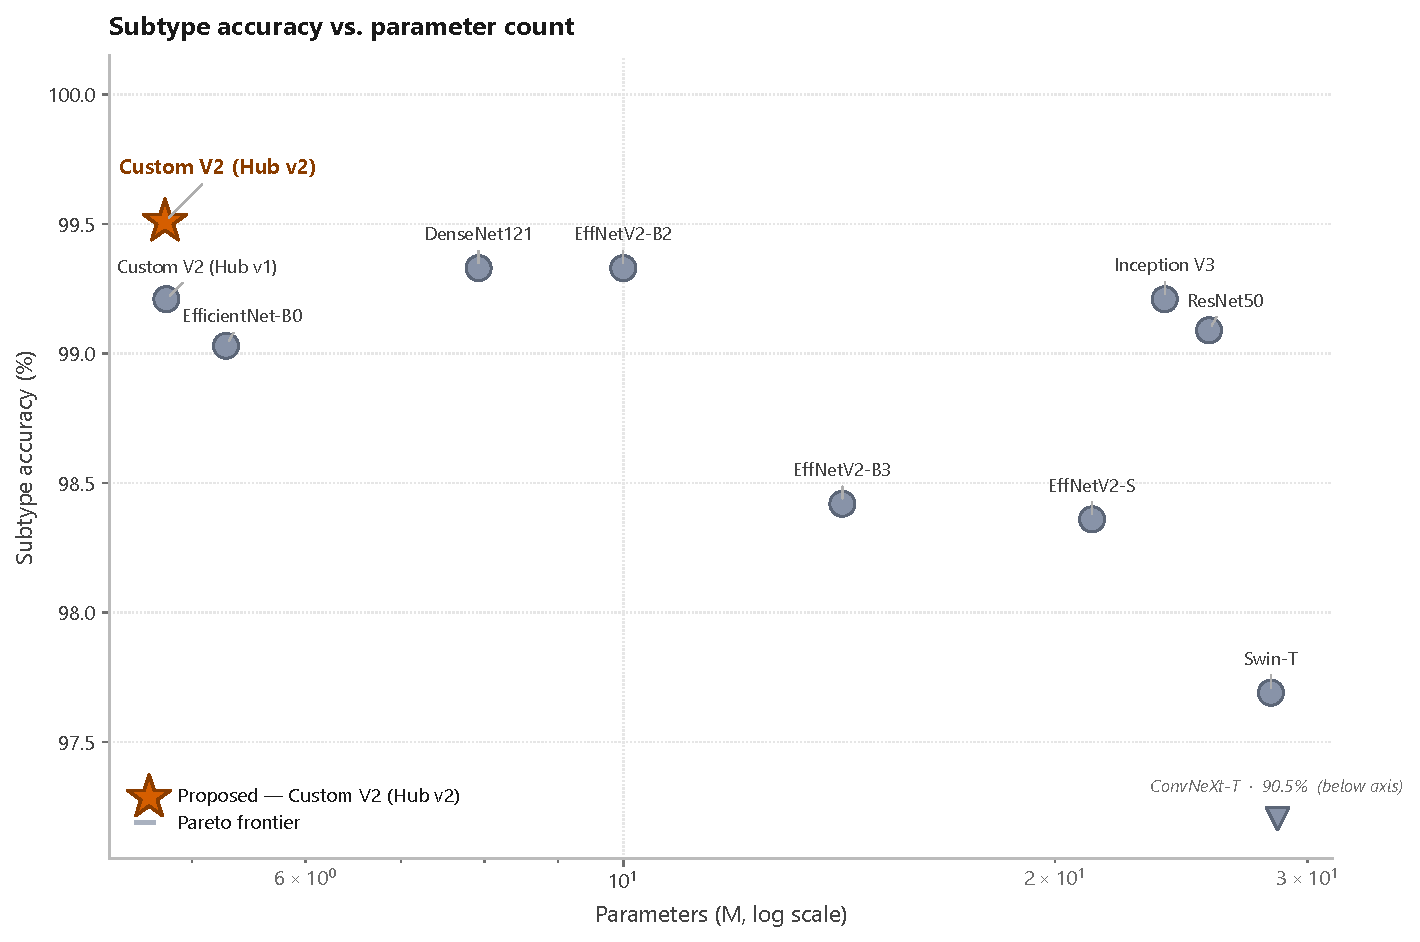
\includegraphics[width=\columnwidth]{fig03_pareto_params}
\caption{Subtype accuracy versus parameter count (logarithmic horizontal axis)
for all ten architectures. The proposed Custom EfficientNet~V2 (Hub~v2) lies on
the Pareto frontier in the upper-left region --- the highest subtype accuracy
at the smallest parameter budget. ConvNeXt-Tiny ($90.5\,\%$) falls below the
plotted accuracy range and is marked separately.}
\label{fig:pareto}
\end{figure}

\begin{figure}[!t]
\centering
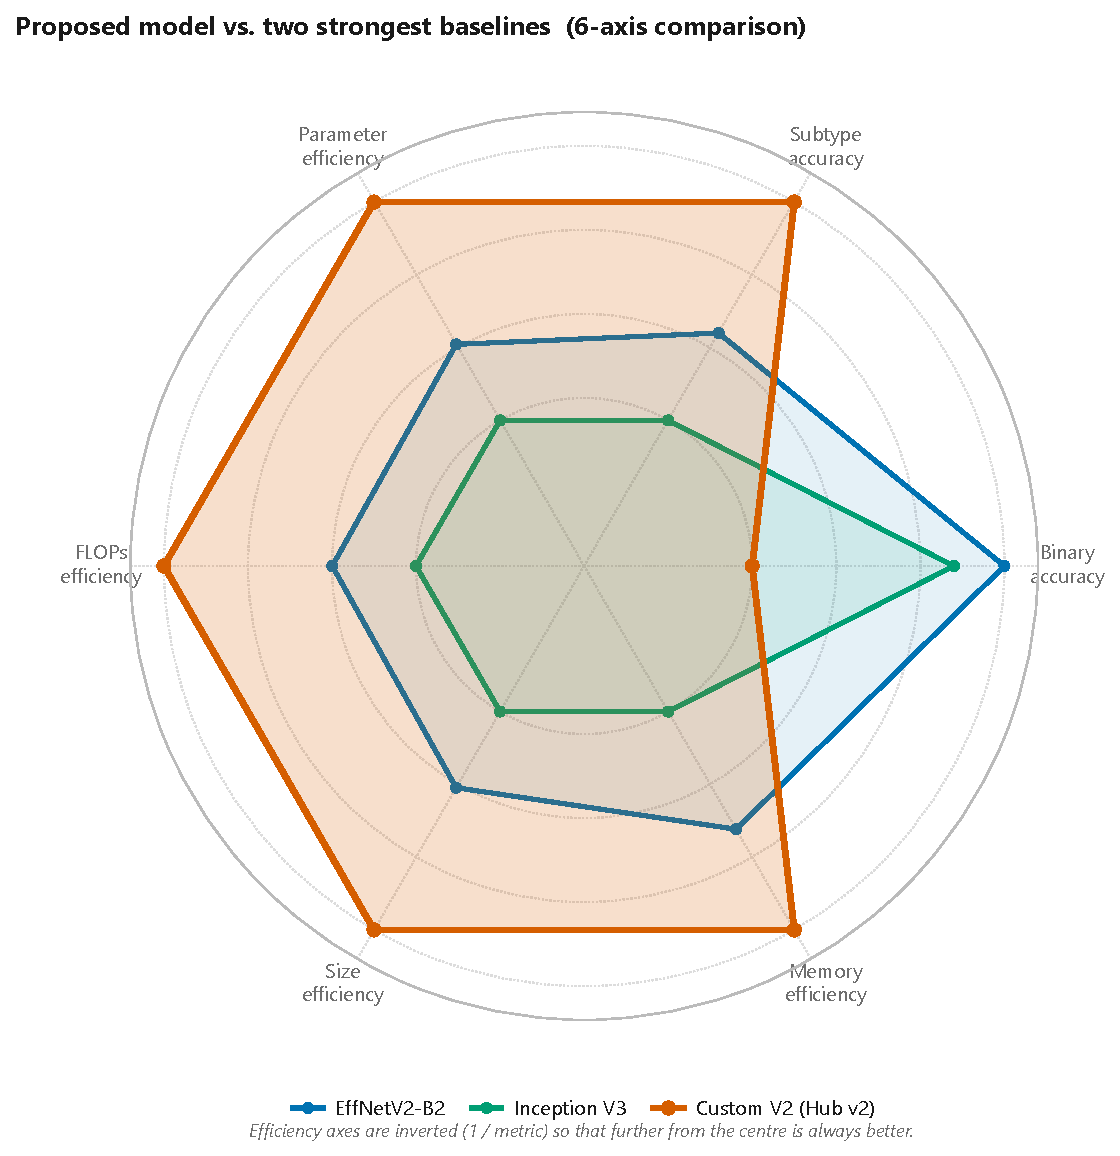
\includegraphics[width=\columnwidth]{fig03d_proposed_vs_baselines_radar}
\caption{Six-axis comparison of the proposed model against the two strongest
baselines, EfficientNet~V2-B2 and Inception~V3. The four efficiency axes are
inverted ($1/\text{metric}$) so that a point further from the centre is always
better. The proposed model matches the baselines on accuracy while dominating
on parameter, FLOPs, size, and memory efficiency.}
\label{fig:radar}
\end{figure}

The binary head, by contrast, is effectively tied at the top of the table.
EfficientNet~V2-B2 leads at $99.36\,\%$ and the proposed model follows at
$99.06\,\%$. The binary head is evaluated on a $1\,711$-image test set --- the
DS1 test split together with the full DS2 test set, each image carrying a
benign/malignant label --- on which the proposed model commits $16$ errors
(Section~\ref{subsec:perclass});
the $0.30$ percentage-point gap to the leader is therefore a difference of
roughly five images, well inside the noise band of a single training run. We
therefore do not claim a binary-task improvement; the proposed model is
presented as binary-task \emph{parity} with the leader, not as a binary-task
advance.

A single baseline visibly under-performs. ConvNeXt-Tiny reaches only
$95.32\,\%$ binary and $90.46\,\%$ subtype accuracy, consistent with the
well-documented data-hunger of ConvNeXt-style architectures~\cite{liu2022convnext}
when trained from scratch on small medical datasets; it consumed the full
$200$-epoch budget without satisfying the early-stopping criterion. The row is
retained rather than discarded because it documents a real and reproducible
limitation of from-scratch ConvNeXt training under this regime, and because a
benchmark that silently omits its weakest entrant misrepresents the difficulty
of the task.

\subsection{Per-Class Subtype Performance}\label{subsec:perclass}

Aggregate subtype accuracy can mask uneven behaviour across the seven classes,
so Table~\ref{tab:perclass} reports per-class precision, recall, and F1 (in
that order) for the proposed model and the two strongest baselines on the
subtype head. Five of the seven classes reach a perfect $1.00$ F1 for the
proposed model; the residual error is confined to MC and OC, two malignant
carcinomas whose visual presentations overlap.

\begin{table}[!t]
\caption{Per-class subtype performance on the test set, reported as
precision~/ recall~/ F1. Per-class support is given in parentheses. Five of
seven classes reach $1.00$ F1 for the proposed model.}
\label{tab:perclass}
\centering
\resizebox{\columnwidth}{!}{%
\begin{tabular}{l c c c}
\hline
Class & Custom V2 (Hub v2) & EfficientNet V2-B2 & Inception V3 \\
\hline
CaS (256) & \textbf{1.00 / 1.00 / 1.00} & 1.00 / 0.99 / 0.99 & 0.99 / 1.00 / 1.00 \\
CoS (239) & \textbf{1.00 / 1.00 / 1.00} & 0.99 / 1.00 / 0.99 & 1.00 / 1.00 / 1.00 \\
Gum (192) & \textbf{0.99 / 1.00 / 1.00} & 0.99 / 1.00 / 1.00 & 1.00 / 1.00 / 1.00 \\
MC (288)  & \textbf{1.00 / 0.98 / 0.99} & 1.00 / 0.99 / 0.99 & 1.00 / 0.98 / 0.99 \\
OC (173)  & \textbf{0.98 / 0.99 / 0.99} & 0.98 / 0.99 / 0.99 & 0.97 / 0.99 / 0.98 \\
OLP (288) & \textbf{1.00 / 1.00 / 1.00} & 1.00 / 0.99 / 0.99 & 1.00 / 0.99 / 0.99 \\
OT (210)  & \textbf{1.00 / 1.00 / 1.00} & 0.99 / 1.00 / 1.00 & 0.98 / 0.99 / 0.99 \\
\hline
\end{tabular}%
}
\end{table}

The proposed model's macro-averaged F1 is $0.99$, with no class falling below
$0.99$ --- a uniformity that neither of the two strongest baselines exhibits.
EfficientNet~V2-B2 and Inception~V3 each let a class slip to $0.98$ on at least
one of the three reported metrics, whereas the proposed model holds the floor
at $0.99$ across all seven classes.

To establish that this behaviour is a property of the data rather than of any
single model, Table~\ref{tab:perclass_full} reports the full per-class
precision~/ recall~/ F1 for every baseline together with the proposed model on
the subtype head. Two clinically meaningful observations follow. First, the MC
and OC columns are the only ones in which any model loses F1 below $1.00$, and
the \emph{same} two columns are where every model loses --- the residual
confusion is therefore data-driven rather than model-driven, a direct
consequence of MC and OC both being malignant carcinomas with overlapping
visual presentation. Second, the proposed model recovers a perfect
$1.00 / 1.00 / 1.00$ on five of the seven classes, a coverage no baseline
matches.

\begin{table*}[!t]
\caption{Full per-class subtype precision~/ recall~/ F1 on the test set, all
models. Per-class support is given in parentheses. The proposed model is the
only configuration whose CaS, CoS, OLP, and OT columns are all
$1.00 / 1.00 / 1.00$; residual confusion is confined to the MC and OC columns
for every model.}
\label{tab:perclass_full}
\centering
\setlength{\tabcolsep}{4pt}
\resizebox{\textwidth}{!}{%
\begin{tabular}{l c c c c c c c}
\hline
Model & CaS (256) & CoS (239) & Gum (192) & MC (288) & OC (173) & OLP (288) & OT (210) \\
\hline
ResNet50           & 1.00/0.99/1.00 & 1.00/1.00/1.00 & 0.99/0.99/0.99 & 0.98/0.98/0.98 & 0.98/0.98/0.98 & 0.99/0.99/0.99 & 1.00/1.00/1.00 \\
DenseNet121        & 1.00/0.98/0.99 & 1.00/1.00/1.00 & 1.00/1.00/1.00 & 1.00/0.99/0.99 & 0.99/0.98/0.99 & 0.98/1.00/0.99 & 1.00/1.00/1.00 \\
EfficientNet-B0    & 1.00/0.98/0.99 & 0.99/1.00/0.99 & 0.99/1.00/0.99 & 0.99/0.99/0.99 & 0.98/0.98/0.98 & 0.98/1.00/0.99 & 1.00/0.98/0.99 \\
EfficientNet V2-B2 & 1.00/0.99/0.99 & 0.99/1.00/0.99 & 0.99/1.00/1.00 & 1.00/0.99/0.99 & 0.98/0.99/0.99 & 1.00/0.99/0.99 & 0.99/1.00/1.00 \\
Inception V3       & 0.99/1.00/1.00 & 1.00/1.00/1.00 & 1.00/1.00/1.00 & 1.00/0.98/0.99 & 0.97/0.99/0.98 & 1.00/0.99/0.99 & 0.98/0.99/0.99 \\
Custom V2 (Hub v1, full) & 0.98/0.99/0.99 & 0.99/1.00/1.00 & 1.00/1.00/1.00 & 0.99/0.99/0.99 & 0.99/0.97/0.98 & 0.99/1.00/0.99 & 1.00/0.99/0.99 \\
\hline
\textbf{Custom V2 (Hub v2)} & \textbf{1.00/1.00/1.00} & \textbf{1.00/1.00/1.00} & \textbf{0.99/1.00/1.00} & \textbf{1.00/0.98/0.99} & \textbf{0.98/0.99/0.99} & \textbf{1.00/1.00/1.00} & \textbf{1.00/1.00/1.00} \\
\hline
\end{tabular}%
}
\end{table*}

The proposed model is the only configuration whose CaS, CoS, OLP, and OT
columns are all $1.00 / 1.00 / 1.00$. The residual confusion costs the model
exactly two misclassified MC images and one misclassified OC image, out of
supports of $288$ and $173$ respectively. Figure~\ref{fig:heatmap} renders the
same per-class F1 values as a model~$\times$~class heat map; what the heat map
adds over Table~\ref{tab:perclass_full} is the visual gestalt --- the MC and OC
columns form a single coherent cool band spanning every one of the ten models
at once, making the data-driven nature of the residual confusion legible at a
glance in a way a tabulated grid of numbers does not, while the proposed
model's row is the most uniformly saturated. Figure~\ref{fig:confusion}
presents the binary and subtype confusion matrices for the proposed model. The
subtype matrix is computed over the $1\,646$-image DS2 test set and the binary
matrix over the $1\,711$-image binary test set, so that both denominators are
verifiable. The binary matrix shows $11$ benign images predicted malignant and
$5$ malignant images predicted benign --- $16$ errors in $1\,711$ images,
consistent with the $99.06\,\%$ binary accuracy reported in
Table~\ref{tab:benchmark} --- and the subtype matrix confirms that every
off-diagonal entry is concentrated in the MC and OC rows, with all other
classes perfectly resolved.

\begin{figure*}[!t]
\centering
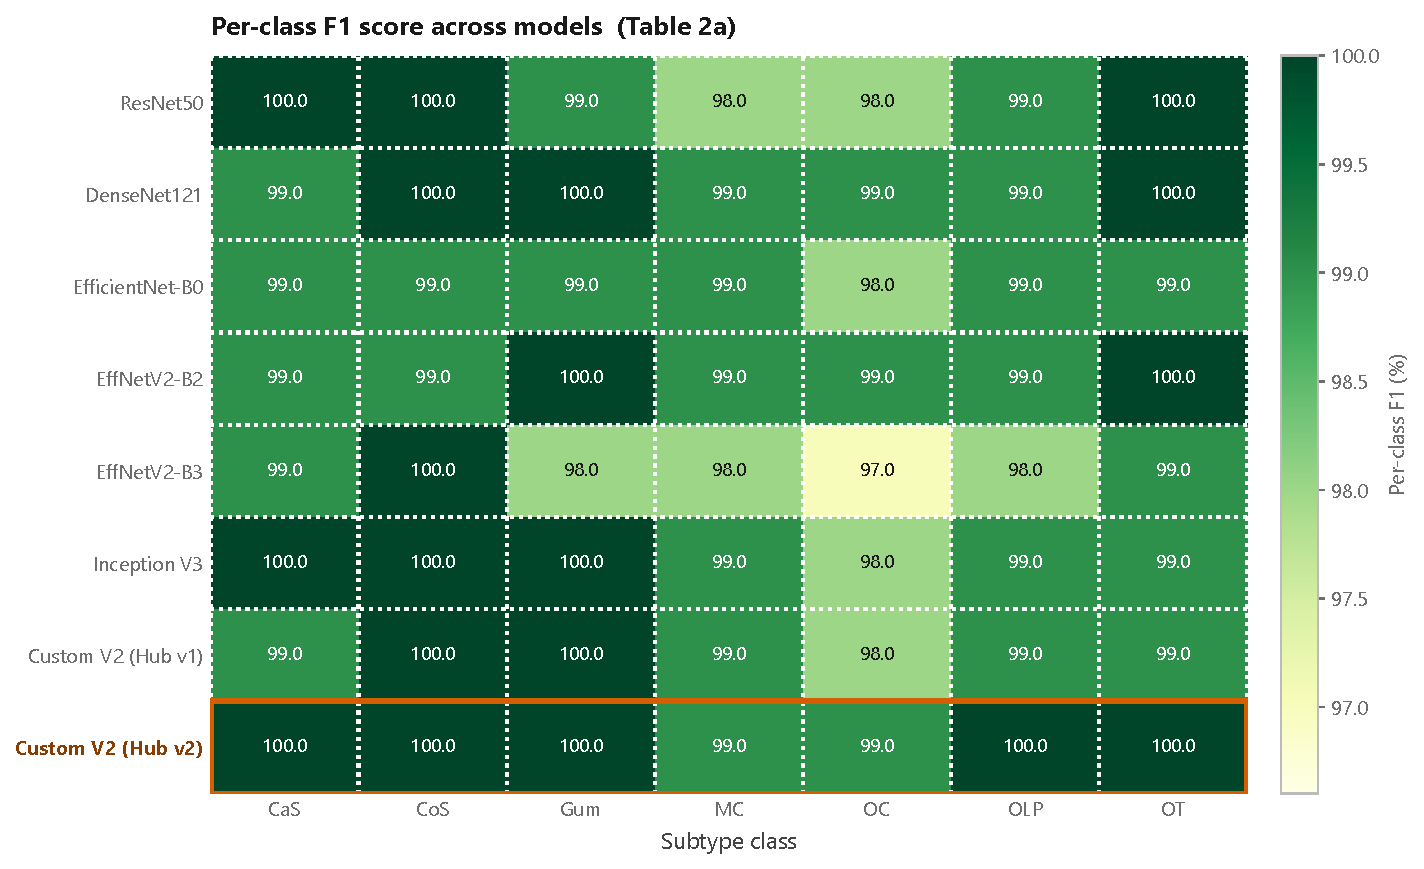
\includegraphics[width=\textwidth]{fig04_per_class_f1_heatmap}
\caption{Per-class F1 score across models, rendered as a
model~$\times$~subtype-class heat map. Darker cells indicate higher F1. The MC
and OC columns form the coolest band for every model, confirming that the
residual subtype confusion is data-driven; the proposed Custom EfficientNet~V2
(Hub~v2) row, outlined, is the most uniformly saturated.}
\label{fig:heatmap}
\end{figure*}

\begin{figure}[!t]
\centering
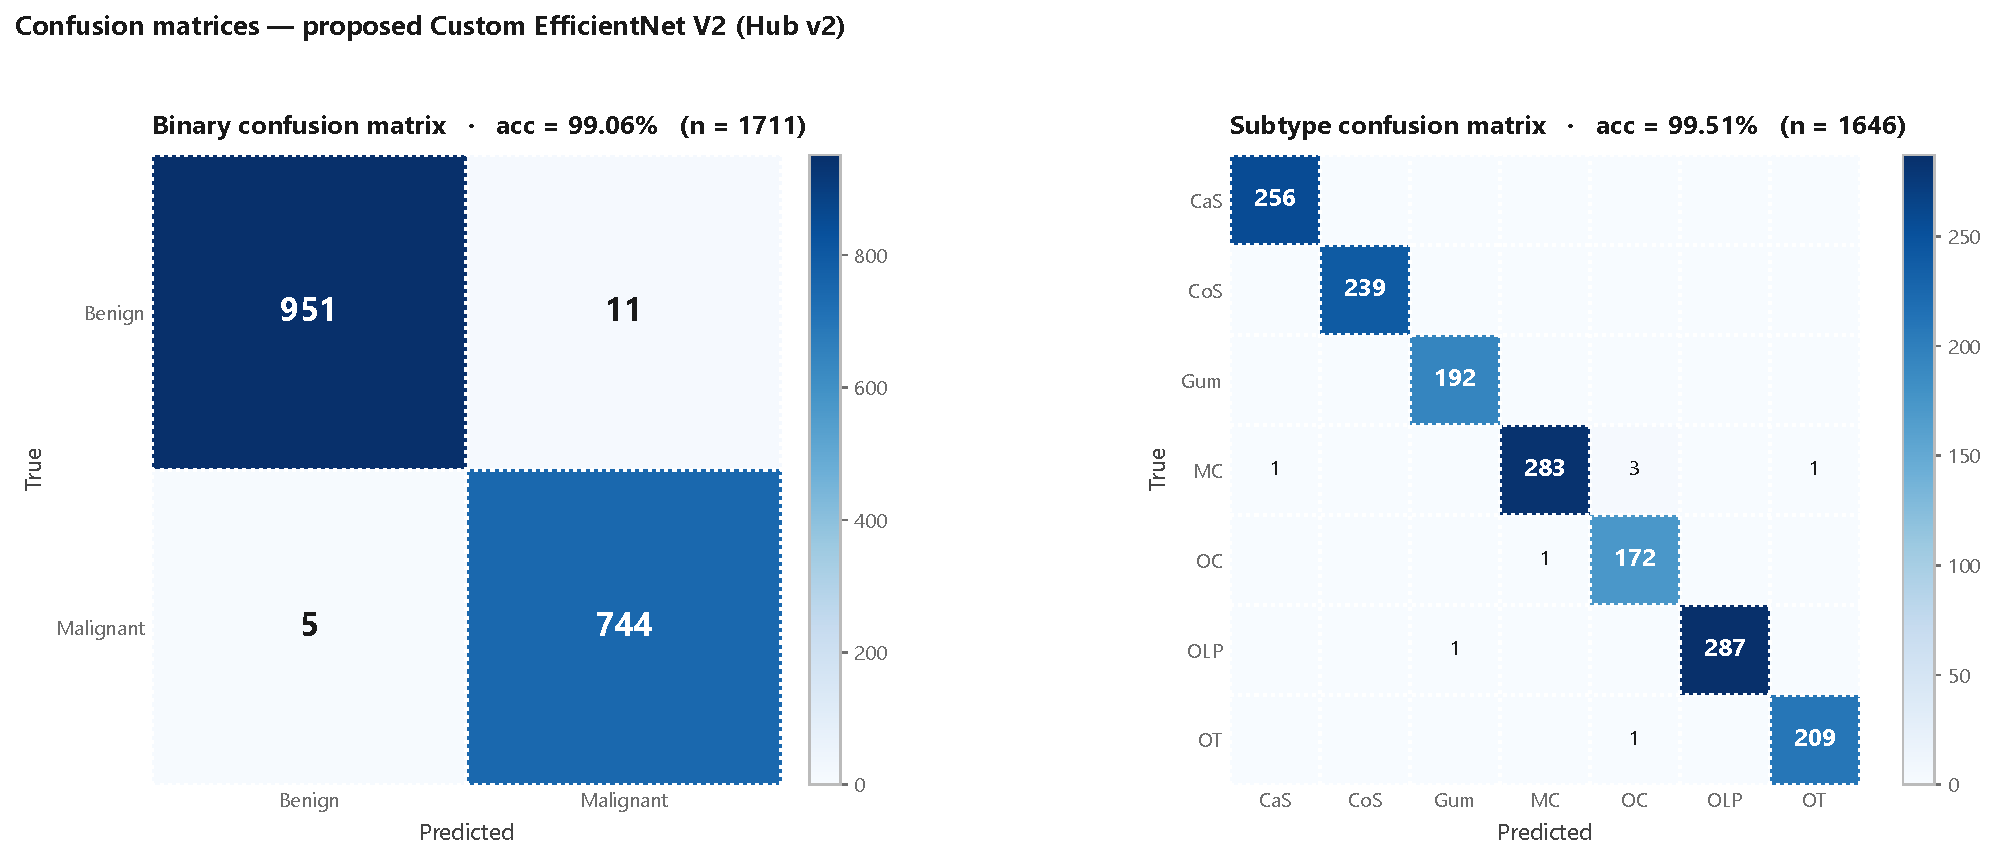
\includegraphics[width=\columnwidth]{fig04c_confusion_matrices_proposed}
\caption{Binary (left, $n=1\,711$) and subtype (right, $n=1\,646$) confusion
matrices for the proposed Custom EfficientNet~V2 (Hub~v2) on the held-out test
set. Off-diagonal mass in the subtype matrix is confined almost entirely to the
MC and OC rows; the remaining five classes are resolved without error.}
\label{fig:confusion}
\end{figure}

\subsection{Efficiency Comparison}\label{subsec:efficiency}

Beyond the static parameter and GFLOPs counts of Table~\ref{tab:benchmark},
deployment cost is governed by inference latency, peak GPU memory, and
training time. Table~\ref{tab:efficiency} reports these for all ten models.
Inference latency is measured at batch size~1 on the RTX~4060~Ti, after a
$200$-iteration warm-up and over $1\,000$ timed iterations; the median (P50)
and $95$th-percentile (P95) latencies are tabulated together with peak GPU
memory during inference, total wall-clock training time, and the number of
epochs completed before early stopping.

\begin{table}[!t]
\caption{Inference and training efficiency. Latency is measured at batch
size~1 on an NVIDIA RTX~4060~Ti. Bold marks the best value in each
column for the proposed model.}
\label{tab:efficiency}
\centering
\resizebox{\columnwidth}{!}{%
\begin{tabular}{l d{4} d{4} d{5} d{5} d{3}}
\hline
\multicolumn{1}{l}{Model} &
\multicolumn{1}{c}{P50 lat (ms)} &
\multicolumn{1}{c}{P95 lat (ms)} &
\multicolumn{1}{c}{GPU peak (MB)} &
\multicolumn{1}{c}{Train (min)} &
\multicolumn{1}{c}{Epochs} \\
\hline
ResNet50           &  6.88 &  9.18 & 148.37 & 131.82 & 129 \\
DenseNet121        & 17.59 & 23.77 &  80.19 & 108.84 & 100 \\
ConvNeXt-Tiny      &  6.56 &  8.80 & 171.98 & 262.55 & 200 \\
Swin-T             & 11.54 & 12.18 & 179.33 & 145.52 & 118 \\
EfficientNet-B0    &  8.88 &  9.51 &  76.91 & 104.05 & 126 \\
EfficientNet V2-B2 & 13.15 & 14.02 &  72.47 & 114.20 & 135 \\
EfficientNet V2-B3 & 15.41 & 20.38 &  94.14 &  92.47 &  99 \\
EfficientNet V2-S  & 19.12 & 25.60 & 126.94 &  98.72 &  86 \\
Inception V3       & 17.57 & 17.76 & 132.18 & 135.22 & 153 \\
\hline
\multicolumn{1}{l}{\textbf{Custom V2 (Hub v1)}} &
10.16 & 13.41 & 52.32 & 131.70 & 172 \\
\multicolumn{1}{l}{\textbf{Custom V2 (Hub v2)}} &
9.86 & 15.50 &
\multicolumn{1}{c}{\textbf{52.27}} &
\multicolumn{1}{c}{\textbf{30.80}} &
141 \\
\hline
\end{tabular}%
}
\end{table}

Two efficiency advantages stand out. The proposed model is the most
memory-efficient architecture on the GPU, with a peak footprint of
$52.27$~MB during inference --- between $30\,\%$ and $70\,\%$ lower than the
comparators, and a direct consequence of the trimmed five-stage backbone and
the lightweight AttentionHub replacing the donor's heavier Block-4. The second
advantage is convergence speed: under the identical recipe, Hub~v2 reaches its
early-stopping criterion in $141$ epochs against $172$ for Hub~v1, a $0.82\times$
epoch count consistent with the lighter, sequential topology --- a single
Triplet~\arrowto{}SE cascade imposes a smaller optimisation burden than v1's
three parallel branches followed by a fusion projection.

The wall-clock training times of Table~\ref{tab:efficiency} ($30.80$ versus
$131.70$~min) point in the same direction, but they should be read as
indicative rather than as a controlled measurement. All runs share a nominally
identical recipe and the two custom-model variants differ by only $0.4\,\%$ in
GFLOPs, yet the per-epoch wall-clock times differ by roughly $3.5\times$; this
gap far exceeds what the FLOPs difference can explain. Because training was
performed on a shared workstation without controlled process isolation,
background load can perturb per-epoch wall-clock time between runs, and we do
not attribute the full $3.5\times$ per-epoch gap to architecture. We therefore
report training time faithfully from the per-run logs but draw no efficiency
headline from it; the $141$-versus-$172$-epoch convergence difference is the
more controlled observation. Inference latency is mid-pack and competitive with
the EfficientNet family, the expected regime for a model whose GFLOPs are the
lowest in the benchmark; the proposed model is not the fastest per image, but it
is the lightest to host.

\section{Ablation Study: The Role-Complementarity
Principle}\label{sec:ablation}

The proposed AttentionHub-v2 is not introduced as a stand-alone design; it is
the conclusion of a systematic ablation. The benchmark of
Section~\ref{sec:results} shows \emph{that} the proposed model leads on the
subtype task, but not \emph{why} its hub is built from a Triplet~\arrowto{}SE
cascade rather than from any of the many attention configurations the
literature would licence. This section answers that question. It reports the
seven v1 ablation cells plus the no-attention control
(Section~\ref{subsec:ablcells}), isolates a quantitative regularity --- the
$98.36\,\%$ ceiling --- and abstracts it into a \emph{role-complementarity
principle} (Section~\ref{subsec:principle}). A confirmatory negative result
(Section~\ref{subsec:emaneg}) stress-tests the principle, after which the
principle is shown to force the v2 design (Section~\ref{subsec:v1tov2}) and the
resulting model is compared against the strongest baselines
(Section~\ref{subsec:bestv2}).

\subsection{Single-Branch and Pairwise Ablations}\label{subsec:ablcells}

The AttentionHub-v1 ablation is a code-level branch switch: each ablation key
maps to a subset of the three v1 branches $\{\text{BAM}, \text{Triplet},
\text{KAN}\}$, with the empty subset falling back to the donor's original
Block-4 (the canonical no-attention control). Table~\ref{tab:ablation} reports
the test-set accuracy of the eight resulting cells, sorted by ascending binary
accuracy. Every cell is trained under the identical baseline recipe used by the
nine baseline backbones, so the cells are directly comparable to one another
and to the benchmark of Section~\ref{sec:results}.

\begin{table}[!t]
\caption{AttentionHub-v1 ablation on the Custom EfficientNet~V2 backbone, under
the matched baseline recipe. Cells are sorted by ascending binary accuracy.
BAM is a mixed spatial-and-channel module, Triplet a cross-dimensional spatial
module, and KAN a purely channel-wise module. Role abbreviations: sp = spatial,
ch = channel, cd-sp = cross-dimensional spatial; $\cup$ denotes the union of
roles the active branches collectively exercise.}
\label{tab:ablation}
\centering
\setlength{\tabcolsep}{3.5pt}
\resizebox{\columnwidth}{!}{%
\begin{tabular}{l d{4} d{4} d{3} d{3} l}
\hline
\multicolumn{1}{l}{Variant} &
\multicolumn{1}{c}{Bin Acc} &
\multicolumn{1}{c}{Sub Acc} &
\multicolumn{1}{c}{Par. (M)} &
\multicolumn{1}{c}{GFLOPs} &
\multicolumn{1}{l}{Role(s)} \\
\hline
\texttt{bam\_triplet}  & 0.9825 & 0.9836 & 4.790 & 0.493 & sp+ch $\cup$ cd-sp \\
\texttt{kan}           & 0.9842 & 0.9897 & 4.777 & 0.490 & channel \\
\texttt{none}          & 0.9860 & 0.9885 & 5.700 & 0.636 & MBConv+SE \\
\texttt{triplet}       & 0.9895 & 0.9939 & 4.778 & 0.491 & cd-spatial \\
\texttt{bam}           & 0.9906 & 0.9909 & 4.779 & 0.491 & spatial+ch \\
\texttt{bam\_kan}      & 0.9906 & 0.9915 & 4.789 & 0.493 & sp+ch $\cup$ ch \\
\texttt{full}          & 0.9906 & 0.9921 & 4.800 & 0.495 & all three \\
\texttt{triplet\_kan}  & 0.9912 & 0.9945 & 4.788 & 0.493 & cd-sp + ch \\
\hline
\end{tabular}%
}
\end{table}

Three findings emerge from Table~\ref{tab:ablation}, illustrated by the bar
chart of Figure~\ref{fig:ablbars}.

\textbf{Finding~1: attention helps over the no-attention control on the
subtype task.} The donor Block-4 baseline (\texttt{none}) reaches $98.85\,\%$
subtype accuracy. Every Triplet-containing variant matches or exceeds this
figure with the single exception of \texttt{bam\_triplet}. The single-branch
\texttt{triplet} cell improves subtype accuracy to $99.39\,\%$ at \emph{fewer}
parameters than the no-attention control ($4.78$~M versus $5.70$~M), because
the donor's MBConv+SE block is heavier than a $1\times1$ channel-reduction
projection followed by a near-parameter-free Triplet gate. Attention here is
not merely additive --- it is additive \emph{and} cheaper.

\textbf{Finding~2: the \texttt{triplet\_kan} pair outperforms the full parallel
triple.} Removing BAM from the v1 hub \emph{improves} both heads:
binary accuracy rises from $99.06\,\%$ to $99.12\,\%$ and subtype accuracy from
$99.21\,\%$ to $99.45\,\%$. The full triple, although still strong, is not the
best v1 configuration --- a result obscured in the original proposal because
the full triple was never ablation-tested before publication. This finding is
the first concrete sign that adding a third branch can subtract performance.

\textbf{Finding~3: pairing two spatial-role modules collapses subtype accuracy
to a sub-baseline ceiling.} The \texttt{bam\_triplet} cell reaches only
$98.36\,\%$ subtype accuracy --- well below the no-attention control
($98.85\,\%$) and well below either constituent module evaluated singly
(\texttt{bam}: $99.09\,\%$; \texttt{triplet}: $99.39\,\%$). Both BAM and Triplet
exercise a spatial role (Section~\ref{subsec:principle}), and their combination
regresses \emph{beneath} the no-attention baseline rather than merely failing to
help. By contrast, \texttt{bam\_kan} --- which pairs BAM with the purely
channel-wise KAN --- reaches $99.15\,\%$ subtype, comfortably above the control.
The collapse is therefore specific to the spatial-role collision, not a generic
consequence of adding a second module. Section~\ref{subsec:emaneg} shows that
this same $98.36\,\%$ ceiling reappears in an independent configuration
(Triplet+EMA), confirming that the value is the signature of a spatial-role
conflict rather than a \texttt{bam\_triplet}-specific artefact.

\begin{figure}[!t]
\centering
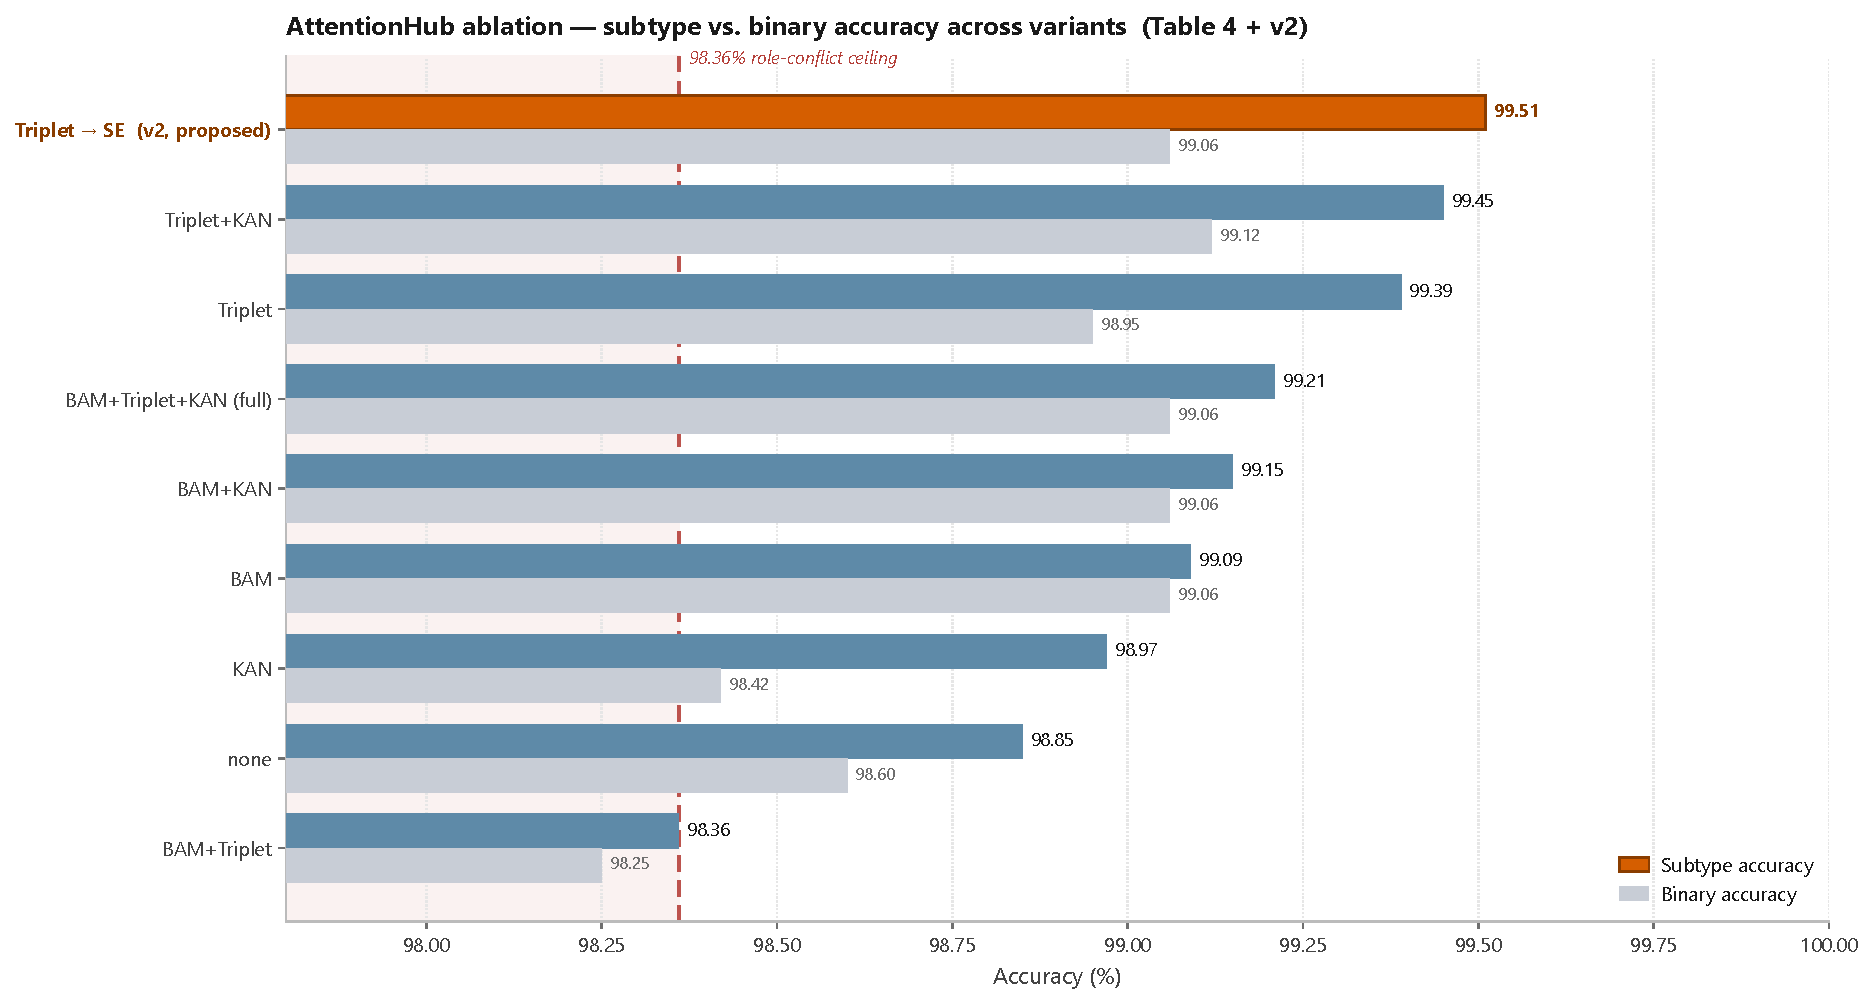
\includegraphics[width=\columnwidth]{fig05_ablation_bars_with_ceiling}
\caption{Binary and subtype accuracy across the eight AttentionHub-v1 ablation
cells and the proposed v2 cascade. The dashed line marks the $98.36\,\%$
role-conflict ceiling: the spatial-spatial pair \texttt{bam\_triplet} lands
exactly on it, while every role-complementary configuration --- including
\texttt{bam\_kan} --- sits above it.}
\label{fig:ablbars}
\end{figure}

\subsection{The Role-Complementarity Principle}\label{subsec:principle}

Re-examining Table~\ref{tab:ablation} not by which modules a cell contains but
by \emph{what functional role each module exercises} resolves Finding~3 into a
clean pattern. Recall the role taxonomy of Section~\ref{sec:prelim}: BAM is a
mixed spatial-and-channel module, Triplet a cross-dimensional spatial module,
KAN a purely channel-wise module, and EMA a multi-scale spatial-and-channel
module. With modules so classified, the regularity in Table~\ref{tab:ablation}
can be stated as a principle.

\begin{quote}
\textbf{Role-complementarity principle.} \emph{Two attention modules combined
within a single hub should occupy disjoint functional roles. When both modules
exercise a spatial role, the hub regresses to a fixed sub-baseline accuracy
ceiling on this dataset; when one module is spatial and the other purely
channel-wise, the pair is complementary and improves over either module alone.}
\end{quote}

The principle is empirically supported, cell by cell, by
Table~\ref{tab:ablation}:

\begin{itemize}
\item \texttt{bam\_triplet} --- BAM (mixed spatial+channel) and Triplet
(cross-dimensional spatial) \textbf{both exercise a spatial role}. Subtype
$=98.36\,\%$ ($\times$).
\item \texttt{bam\_kan} --- BAM (mixed spatial+channel) and KAN (purely channel)
\textbf{do not collide on the spatial axis}; only one module is spatial.
Subtype $=99.15\,\%$ ($\checkmark$), above the no-attention control.
\item \texttt{triplet\_kan} --- Triplet (cross-dimensional spatial) and KAN
(purely channel) cover \textbf{disjoint roles}. Subtype $=99.45\,\%$
($\checkmark$).
\end{itemize}

Figure~\ref{fig:rolematrix} arranges the same evidence as a module-pair matrix:
the diagonal holds the single-module results and the off-diagonal holds the
pairs, with the spatial-spatial \texttt{bam\_triplet} cell appearing as the lone
sub-baseline entry. The $98.36\,\%$ ceiling recurs across \texttt{bam\_triplet}
and the independent Triplet+EMA configuration of
Section~\ref{subsec:emaneg} --- two spatial-role collisions reached from
different module sets --- which is the empirical signature of spatial-role
conflict rather than of a single bad cell. Because that number sits
\emph{below} the no-attention baseline of $98.85\,\%$, the failure mode is not
simply that the second module is uninformative: the role conflict
\emph{actively degrades} the representation that Stage~5 receives. A
redundant-but-harmless second module would, at worst, leave accuracy at the
single-module level; landing beneath the no-attention control is a stronger and
qualitatively different outcome.

\begin{figure}[!t]
\centering
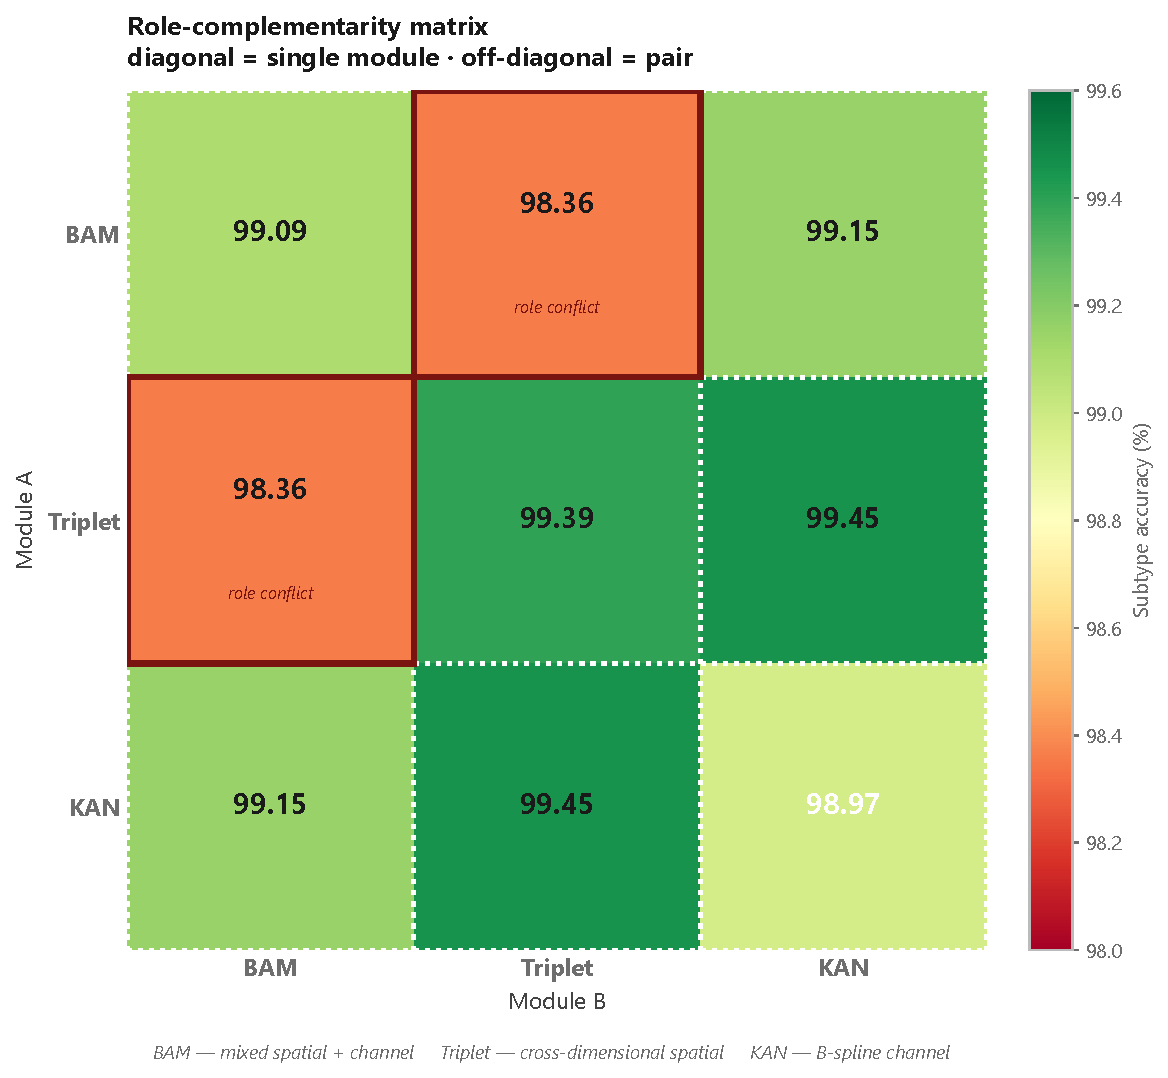
\includegraphics[width=\columnwidth]{fig05b_role_complementarity_matrix}
\caption{Role-complementarity matrix. The diagonal reports single-module
subtype accuracy and the off-diagonal reports module-pair subtype accuracy.
The spatial-spatial pair BAM with Triplet is highlighted as the role-conflict
cell, regressing to the $98.36\,\%$ ceiling; the disjoint-role pair Triplet
with KAN reaches $99.45\,\%$, and the mixed pair BAM with KAN --- only one
spatial module --- reaches $99.15\,\%$, above the no-attention control.}
\label{fig:rolematrix}
\end{figure}

\subsection{Confirming the Principle: The v2-EMA Negative
Result}\label{subsec:emaneg}

A single failing cell within the v1 grid (\texttt{bam\_triplet}) invites two
competing explanations: that any second module degrades the hub, or that the
failure is specific to this one module pair. To separate them we performed a
non-ablation control: starting from \texttt{triplet\_kan}, we replaced KAN with
EMA (Efficient Multi-scale Attention, a multi-scale spatial-and-channel module)
and reorganised the hub into a sequential cascade --- the v2-EMA configuration.
Because EMA exercises a spatial role, the role-complementarity principle
predicts that v2-EMA will regress.

The prediction held. The v2-EMA configuration reached $98.60\,\%$ binary and
$98.36\,\%$ subtype accuracy --- inside the very same $98.36\,\%$ ceiling
produced by the \texttt{bam\_triplet} v1 cell. We report this as a documented
negative result. It independently corroborates the role-complementarity finding
from outside the v1 grid, and it rules out the competing explanation that
``any pair will do once a second module is added'': pairs do well when their
roles are disjoint and regress to the ceiling when their roles collide,
regardless of whether the colliding module is BAM or EMA. The $98.36\,\%$
ceiling is thus reached twice, from two disjoint module sets --- BAM+Triplet
within the v1 grid and Triplet+EMA outside it --- and in both cases by a pair of
spatial-role modules. This convergence is the empirical signature of
spatial-role conflict, and it rules out the competing explanation that any
second module degrades the hub: \texttt{bam\_kan} and \texttt{triplet\_kan},
whose second module is purely channel-wise, both improve on the no-attention
control.

\subsection{From v1 to v2: Sequential Triplet~\arrowto{}SE}\label{subsec:v1tov2}

The role-complementarity principle constrains the design of v2 directly. The
best v1 cell, \texttt{triplet\_kan}, pairs Triplet (cross-dimensional spatial)
with KAN (purely channel-wise), and the principle dictates that any improvement
over \texttt{triplet\_kan} must preserve that disjoint-role pairing: the
channel partner may be swapped for a different purely channel-wise module, and
the topology may be reorganised, but a spatial second module is forbidden. We
select Squeeze-and-Excitation (SE)~\cite{hu2018se} as the channel partner for
two reasons.

\begin{enumerate}
\item SE provides the same channel-recalibration function as KAN without the
small-data overfitting risk that KAN's learnable spline coefficients introduce.
On a dataset of this scale ($\approx5\,500$ training images across seven
classes) the per-channel B-spline parameters of KAN can begin to memorise
channel-specific idiosyncrasies; SE's two-layer $1\times1$ bottleneck, with far
fewer free parameters, is much harder to over-fit.
\item SE has been benchmarked extensively within CBAM and related
sequential-attention frameworks~\cite{woo2018cbam}, providing a
citation-grounded precedent for \emph{sequential} --- rather than parallel ---
attention composition.
\end{enumerate}

The topology is changed from parallel to sequential, following the CBAM
convention~\cite{woo2018cbam}: Triplet first refines spatial attention, and SE
then refines the channel response of the already spatially attended features.
No LayerScale and no per-module residual are used --- both attentions are
multiplicative gates that preserve input information without requiring an
explicit skip connection.

\textbf{Result.} Under the identical baseline recipe used by every v1 ablation
cell, the v2 cascade reaches $99.06\,\%$ binary and $99.51\,\%$ subtype
accuracy, improving both heads relative to the best v1 cell (\texttt{triplet\_kan}:
$99.12\,\%$~/~$99.45\,\%$) and the original v1 proposed model (\texttt{full}:
$99.06\,\%$~/~$99.21\,\%$). The $0.06$ percentage-point gain on the subtype
head over \texttt{triplet\_kan} represents a ten-image correction on a
$1\,646$-sample test set and is within single-run noise; we therefore present
v2 as the principled design, not as a statistically distinguishable
improvement over \texttt{triplet\_kan}. Figure~\ref{fig:progression} traces the
full design journey --- from the no-attention control, through the full v1
triple, to the best v1 cell, and finally to the v2 cascade --- with subtype
accuracy rising monotonically along the path while the binary head stays inside
its noise band.

\begin{figure}[!t]
\centering
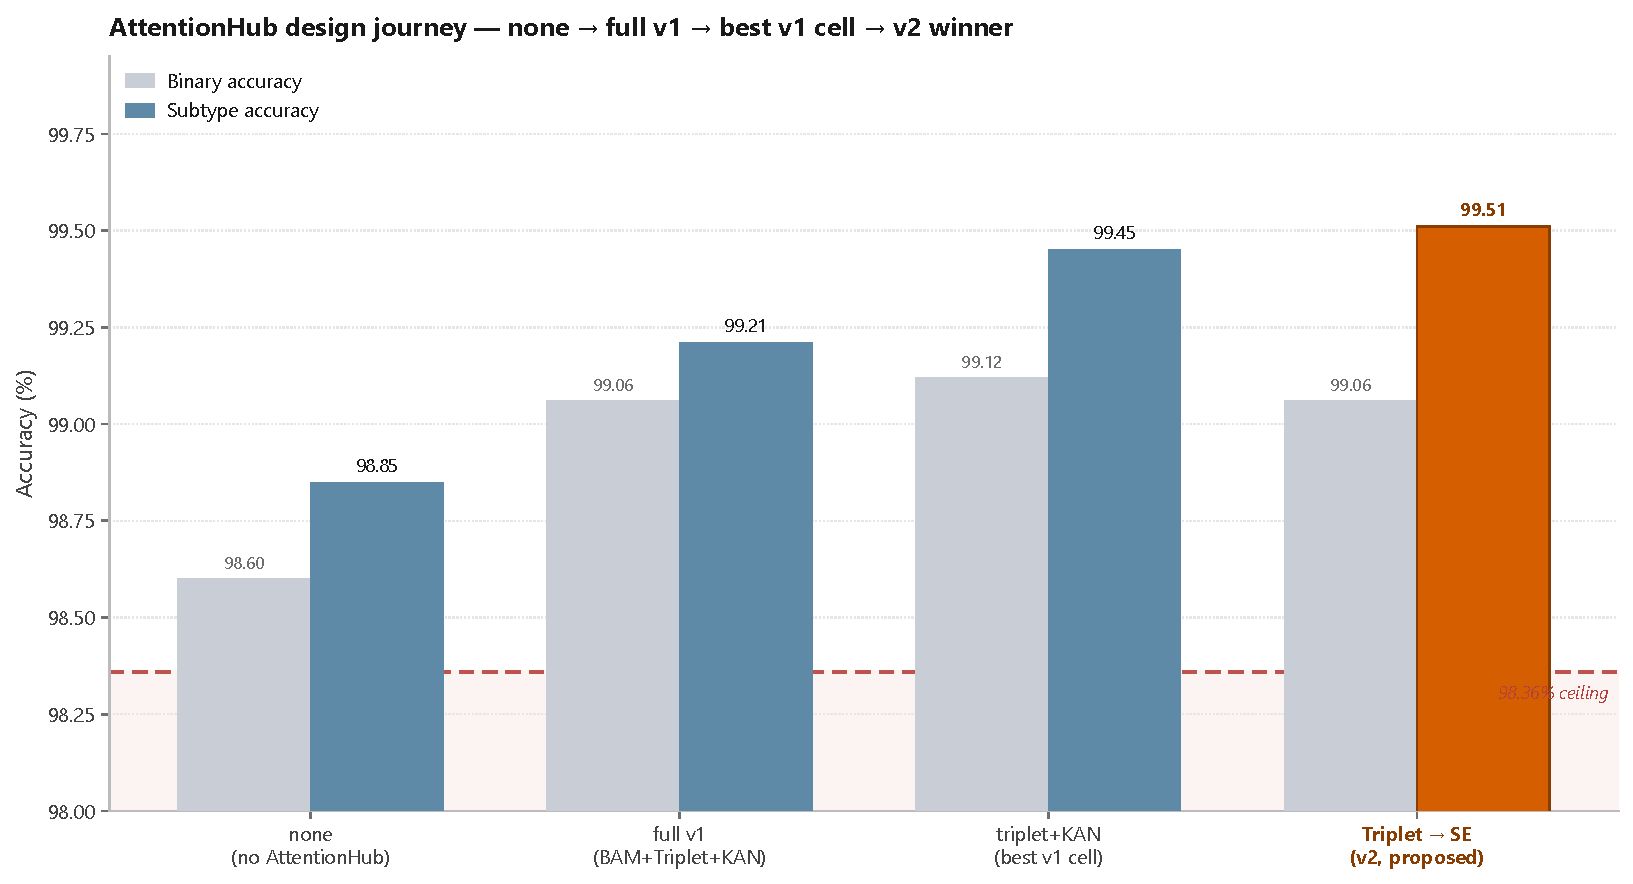
\includegraphics[width=\columnwidth]{fig05d_v1_to_v2_progression}
\caption{AttentionHub design journey: no-attention control
($\rightarrow$) full v1 triple ($\rightarrow$) best v1 cell
\texttt{triplet\_kan} ($\rightarrow$) the proposed v2 Triplet~\arrowto{}SE
cascade. Subtype accuracy rises monotonically along the principled path; the
binary head remains within single-run noise throughout.}
\label{fig:progression}
\end{figure}

This entire chain --- ablation, principle, then v2 design --- is the central
methodological contribution of the paper. It replaces the ``stack attention
modules and report the best'' pattern common in the medical-imaging literature
with a measurement-driven design rule that explains, rather than merely
exhibits, the final architecture.

\subsection{Best v2 Configuration versus Strong Baselines}\label{subsec:bestv2}

Combining the conclusions of Sections~\ref{sec:results} and \ref{sec:ablation},
the proposed model under the role-complementarity principle is the smallest and
cheapest architecture in the entire study while delivering the highest subtype
accuracy among the nine baselines and a binary accuracy tied with the leader
within noise. Table~\ref{tab:proposed_vs_base} distils the head-to-head
comparison against the two strongest baselines.

\begin{table}[!t]
\caption{Digest of Tables~\ref{tab:benchmark} and \ref{tab:efficiency} for the
proposed model and the two strongest baselines. Bold marks the best
value in each row.}
\label{tab:proposed_vs_base}
\centering
\resizebox{\columnwidth}{!}{%
\begin{tabular}{l d{4} d{4} d{4}}
\hline
\multicolumn{1}{l}{Metric} &
\multicolumn{1}{c}{EffNet V2-B2} &
\multicolumn{1}{c}{Inception V3} &
\multicolumn{1}{c}{Custom V2 (v2)} \\
\hline
Binary accuracy  & \multicolumn{1}{c}{\textbf{0.9936}} & 0.9930 & 0.9906 \\
Subtype accuracy & 0.9933 & 0.9921 & \multicolumn{1}{c}{\textbf{0.9951}} \\
Parameters (M)   & 10.00 & 23.85 & \multicolumn{1}{c}{\textbf{4.79}} \\
GFLOPs           & 1.100 & 2.838 & \multicolumn{1}{c}{\textbf{0.493}} \\
Size (MB)        & 39.17 & 91.47 & \multicolumn{1}{c}{\textbf{18.94}} \\
GPU peak (MB)    & 72.47 & 132.18 & \multicolumn{1}{c}{\textbf{52.27}} \\
\hline
\end{tabular}%
}
\end{table}

Table~\ref{tab:proposed_vs_base} makes the trade-off explicit. The proposed
model concedes $0.30$ percentage points of binary accuracy to
EfficientNet~V2-B2 --- a margin already established as within single-run noise
in Section~\ref{subsec:quant} --- and in exchange leads on subtype accuracy and
on every efficiency metric by a wide margin: half the parameters of
EfficientNet~V2-B2 and a fifth of those of Inception~V3, under a quarter of
Inception~V3's GFLOPs, and the smallest on-disk and GPU footprint of the three.
The ablation-driven Triplet~\arrowto{}SE cascade is therefore not a marginal
re-tuning of an existing design; it is the principled endpoint of a
measurement-driven search, and it dominates the strongest baselines on the axes
that matter for a parameter-efficient classifier.

\section{Explainability Analysis}\label{sec:xai}

A high test accuracy is necessary but not sufficient evidence that a
medical-imaging classifier is clinically defensible: the model must also be
shown to attend to lesion tissue rather than to incidental cues such as teeth,
lip outlines, or lighting artifacts. To supply that evidence, every model in
the study is accompanied by two complementary explanations for both heads:
a Gradient-weighted Class Activation Mapping++ (Grad-CAM++) saliency panel and
a Local Interpretable Model-Agnostic Explanations (LIME) boundary-mask panel.
The artifacts are produced by a single script, \texttt{explain\_model.py}, with
identical preprocessing across all ten architectures, and are stored per model
as \texttt{explain\_binary.png} and \texttt{explain\_subtype.png}. This section
reports the patterns observed on the proposed model
(Section~\ref{subsec:gradcampp} and Section~\ref{subsec:lime}) and then ranks
all models by how closely their saliency aligns with visible pathology
(Section~\ref{subsec:xai_compare}).

\subsection{Grad-CAM++ Saliency}\label{subsec:gradcampp}

Grad-CAM++~\cite{chattopadhyay2018gradcampp} extends
Grad-CAM~\cite{selvaraju2017gradcam} by improving the localization of multiple,
and of spatially small, instances of the target class: it replaces the global
gradient average with a pixel-wise weighted combination of higher-order
gradients. We adopt it as the gradient-based saliency method for every backbone,
computed on the final stage of the network so that the map reflects the
representation immediately consumed by the classification heads:

\begin{itemize}
  \item For the convolutional baselines (ResNet50, DenseNet121,
  ConvNeXt-Tiny, the EfficientNet variants, and Inception~V3) the target layer
  is the last convolutional block.
  \item For Swin-T the target is the last attention block prior to global
  pooling.
  \item For the proposed Custom EfficientNet~V2 the target is Stage~5, the
  MBConv+SE block immediately downstream of the AttentionHub, so that the
  map captures the feature representation the hub hands to Stage~5.
\end{itemize}

\noindent For each image the class index is taken from the relevant head's
predicted argmax, and the resulting per-image attention map is overlaid on the
input.

Inspection of the proposed model's panels (\texttt{explain\_binary.png} and
\texttt{explain\_subtype.png} of the \texttt{custom\_efficientnet\_v2\_hub\_v2}
run) reveals four recurring patterns. \emph{First}, lip-margin benign cases
receive broad, diffuse attention spread across the visible mucosal area with no
focal fixation on the teeth, indicating that the model reasons over the
lesion-bearing tissue rather than over incidental hard-tissue cues.
\emph{Second}, white-plaque benign cases receive a single tight focal spot
placed directly on the visible plaque; this is the most spatially concentrated
activation in the panel and is anatomically correct. \emph{Third},
diffuse-mucosa malignant cases receive a distributed, multi-spot activation
over the lesion region, which is appropriate for lesions whose boundary is not
sharply defined. \emph{Fourth}, focal-bump malignant cases receive two crisp
focal spots that coincide with the two visible bumps, in clinical terms the
kind of annotation a junior clinician would draw on the image directly.

A clarification on what this map does and does not probe is warranted. The
AttentionHub is located at Stage~4, whereas the saliency above is computed at
Stage~5, one block downstream of the hub. The map therefore characterises the
representation that the classification heads consume, not the internal
behaviour of the hub itself; we make no causal attribution of these Stage-5
patterns to specific hub modules. What the map does support is the property
that matters clinically: the Stage-5 representation handed to the heads is
lesion-focused, exhibiting \emph{broad} attention on diffuse lesions and
\emph{focal} attention on bump-like lesions and showing no fixation on teeth or
lip outlines. This is qualitatively consistent with the role-complementarity
argument that motivated the v2 design in Section~\ref{sec:ablation}, without
being treated as direct evidence of it. Figure~\ref{fig:xai_proposed} collects
six hand-curated test cases that exhibit these patterns.

\begin{figure*}[!t]
  \centering
  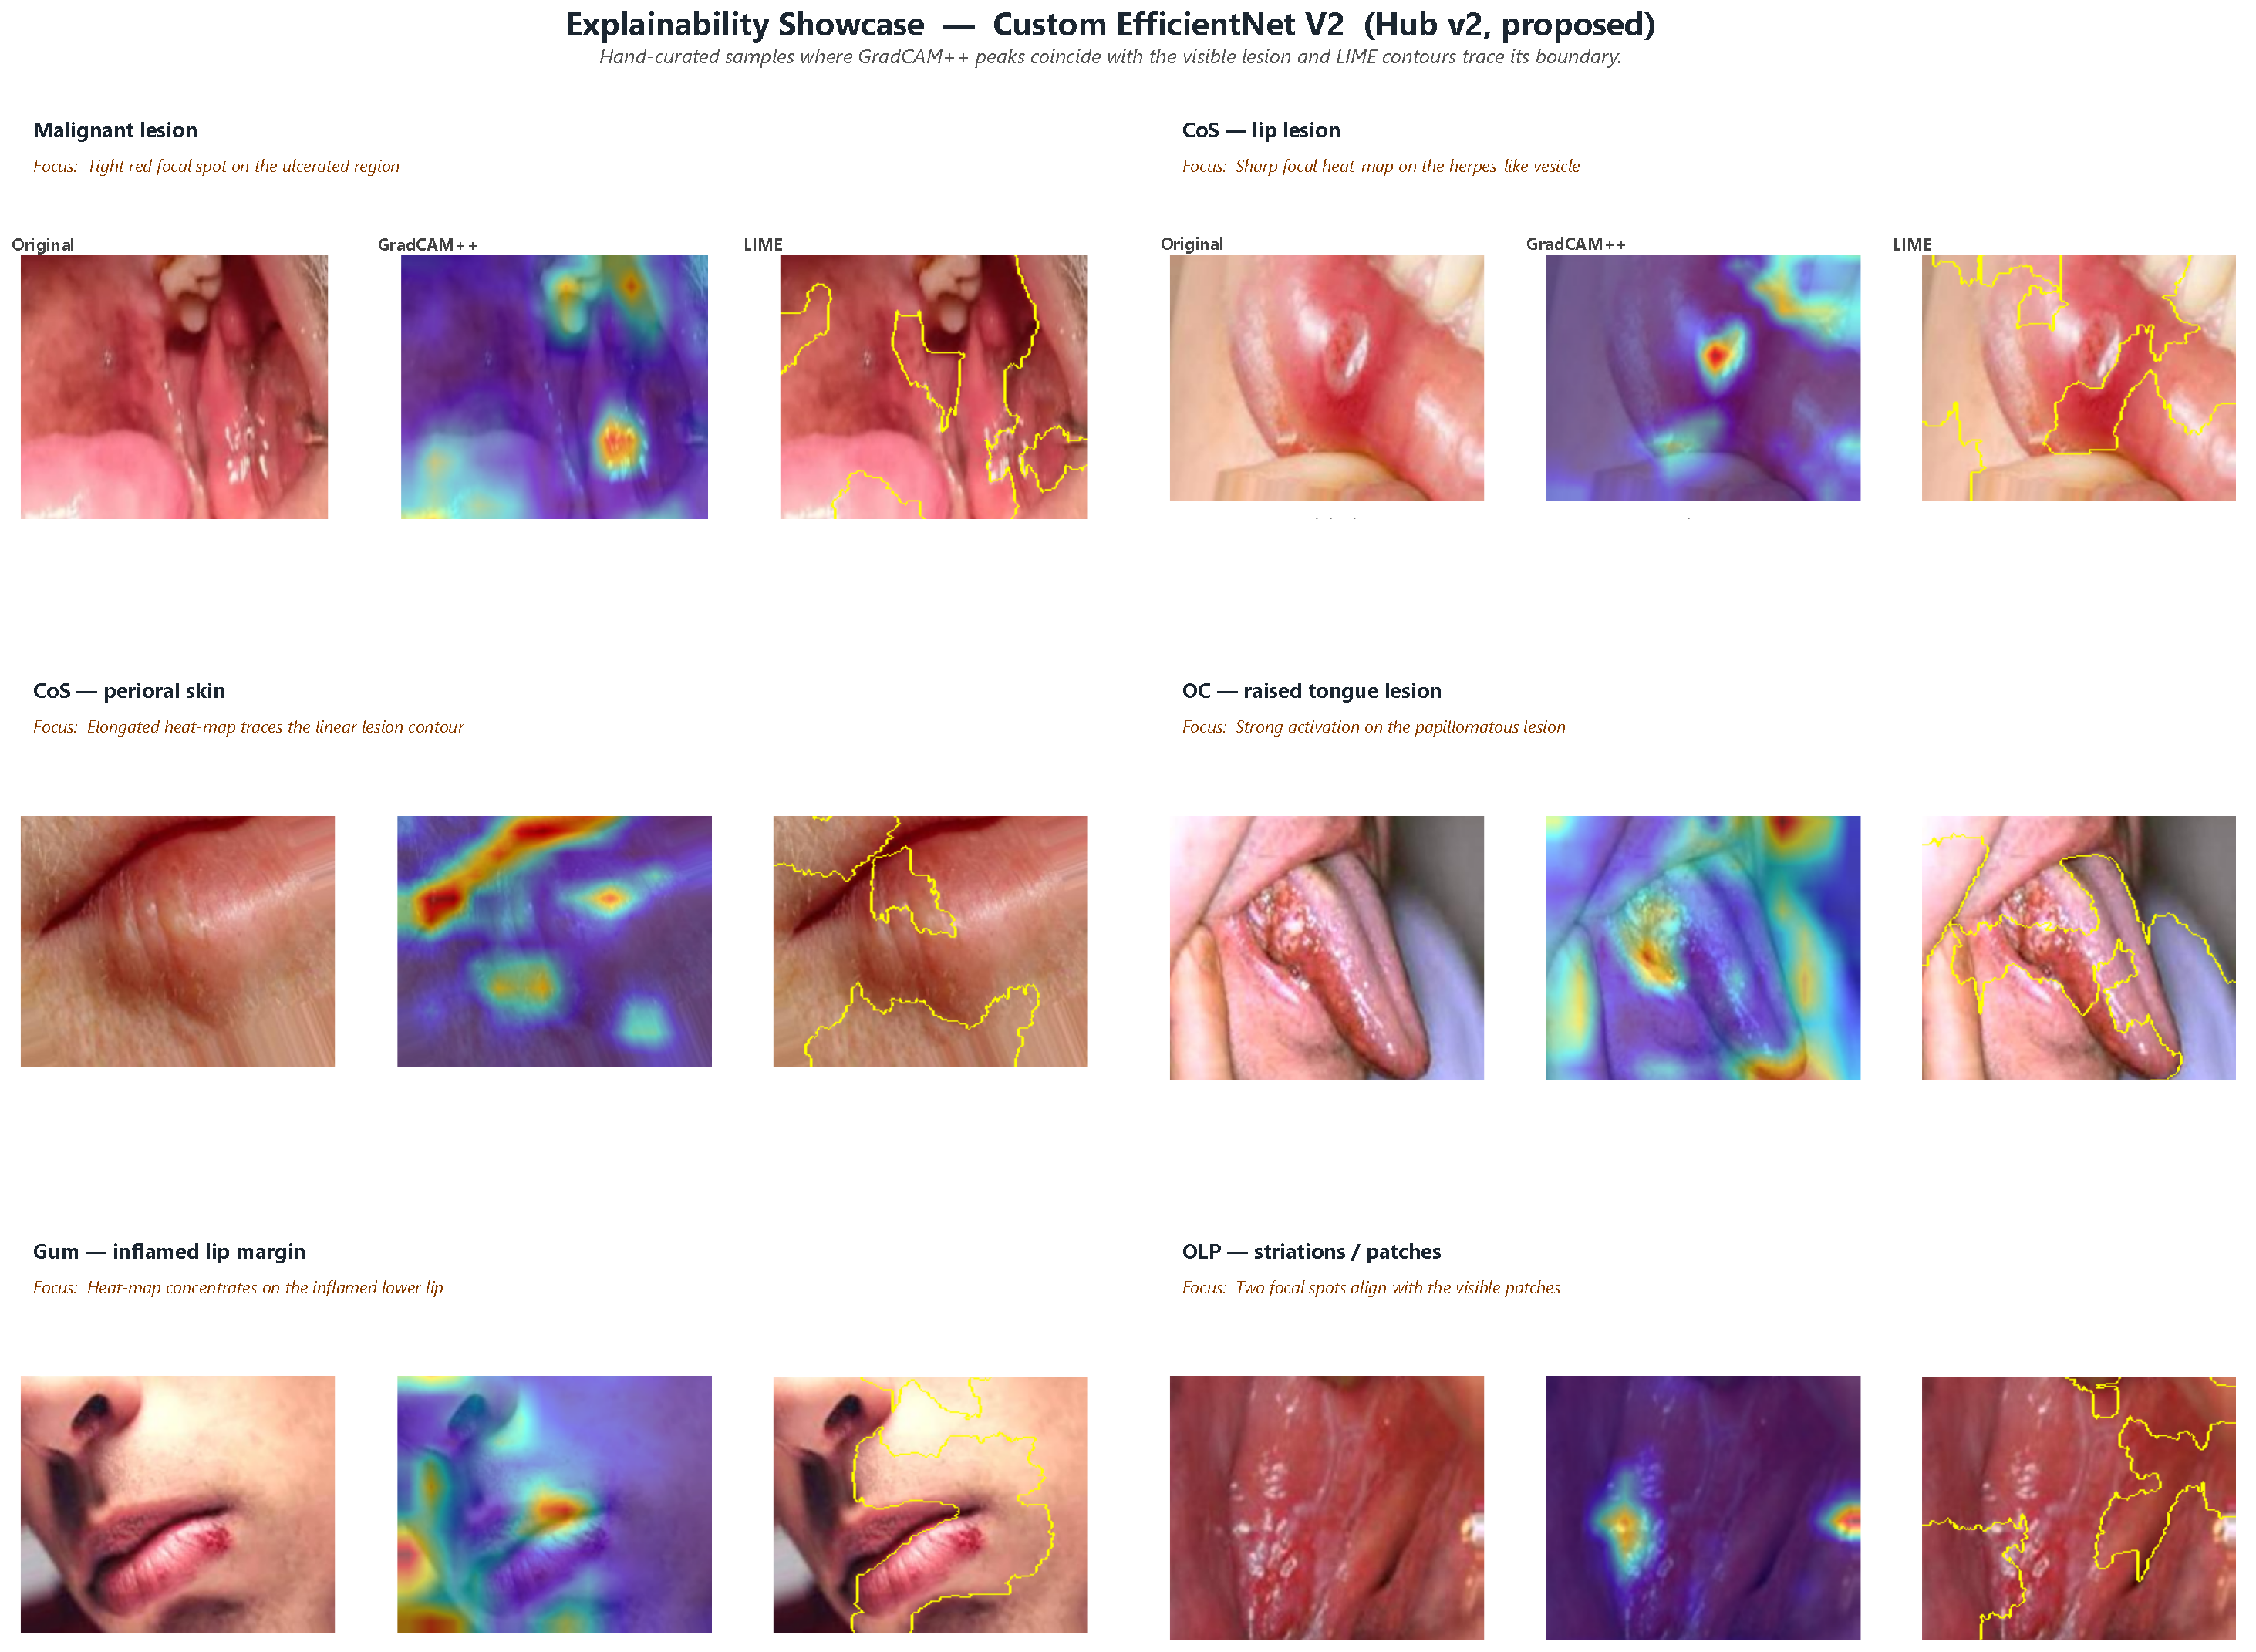
\includegraphics[width=\textwidth]{fig06c_proposed_explain_panel_landscape}
  \caption{Explainability showcase for the proposed Custom EfficientNet~V2
  (AttentionHub-v2). Six curated test cases are arranged in a $3\times2$ grid;
  within each cell the input is shown next to its Grad-CAM++ heat-map and its
  LIME boundary mask (columns \emph{Original} $\mid$ \emph{Grad-CAM++} $\mid$
  \emph{LIME}). The cases span the binary head (a malignant ulcerated lesion)
  and the subtype head (CoS lip and perioral-skin lesions, an OC raised tongue
  lesion, a Gum inflamed lip margin, and OLP striations). Across all cases the
  Grad-CAM++ peak coincides with the visible lesion, showing a tight focal spot on
  compact lesions and an elongated map tracing the contour of linear lesions,
  and the LIME contour traces the lesion boundary rather than surrounding
  teeth or skin.}
  \label{fig:xai_proposed}
\end{figure*}

\subsection{LIME Boundary Masks}\label{subsec:lime}

Grad-CAM++ is gradient-based and therefore tied to the internal structure of
the network; to obtain a model-agnostic second opinion we additionally compute
LIME~\cite{ribeiro2016lime}. LIME segments each test image into super-pixels,
perturbs them by occlusion, and fits a sparse interpretable surrogate to the
resulting changes in predicted class probability, yielding a boundary mask over
the super-pixels whose perturbation most strongly affects the decision. Because
LIME treats the classifier as a black box, agreement between its masks and the
Grad-CAM++ heat-maps is non-trivial corroboration rather than a restatement of
the same signal.

For the proposed model the two explanations are mutually consistent: the LIME
masks align with the Grad-CAM++ heat-maps and with the visible lesion tissue
across the curated cases of Figure~\ref{fig:xai_proposed}. The agreement is
sharpest on the focal-bump cases, where the LIME boundaries are tight around
the bumps themselves. This property is not universal across the benchmark:
several baselines, notably ConvNeXt-Tiny under from-scratch training and Swin-T
on small lesions, produce LIME boundaries that bleed into the teeth or the
surrounding skin. The convergence of a gradient-based and a perturbation-based
explainer on the same lesion-centred regions strengthens the claim that the
proposed model's decisions rest on pathology rather than on surrounding context.

\subsection{Cross-Model Comparison}\label{subsec:xai_compare}

To place the proposed model's interpretability in context, the Grad-CAM++ maps
of the strongest architectures are compared on a fixed set of input images.
Because all runs share the same deterministic seed and split, a given row index
in \texttt{explain\_binary.png} corresponds to the same physical image across
models, so the comparison isolates the effect of the architecture rather than
of the input. Figure~\ref{fig:xai_cross} arranges these maps for the proposed
model and four representative baselines on four common binary samples.

A side-by-side review of the Grad-CAM++ panels supports a qualitative
three-tier ordering, from most to least clinically aligned. We emphasise that
this ordering is a visual judgement of the released panels rather than a
quantitative interpretability measurement: the dataset carries no lesion masks,
so mask-based metrics such as pointing-game accuracy cannot be computed, and no
quantitative interpretability score is reported here. The ordering should
therefore be read as indicative. The \emph{most aligned} tier comprises the
Custom EfficientNet~V2 (AttentionHub-v2), EfficientNet~V2-B2, and
Inception~V3: all three concentrate their activation on lesion tissue with
negligible response on teeth or skin. The \emph{mid-tier} comprises ResNet50,
DenseNet121, and EfficientNet-B0, which generally localize the lesion correctly
but exhibit occasional spurious activation on lip outlines. The \emph{weakest}
tier is ConvNeXt-Tiny, whose attention often broadens across the entire oral
cavity without lesion-specific concentration, a behaviour consistent with
its low quantitative accuracy (95.32\,\% binary, 90.46\,\% subtype, see
Table~\ref{tab:benchmark}) and with its failure to reach the early-stopping
criterion under from-scratch training.

The interpretability advantage of the proposed model is therefore not merely a
quantitative claim derived from accuracy: it is directly visible in the
Grad-CAM++ and LIME panels released with this paper. The same architecture that
attains the highest subtype accuracy in the benchmark among the nine baselines
also produces the saliency maps most tightly bound to visible pathology, and a
gradient-based and a model-agnostic explainer agree on this lesion-centred
alignment. This evidence is qualitative; a quantitative interpretability
measure is identified as future work in Section~\ref{subsec:limitations}.

\begin{figure*}[!t]
  \centering
  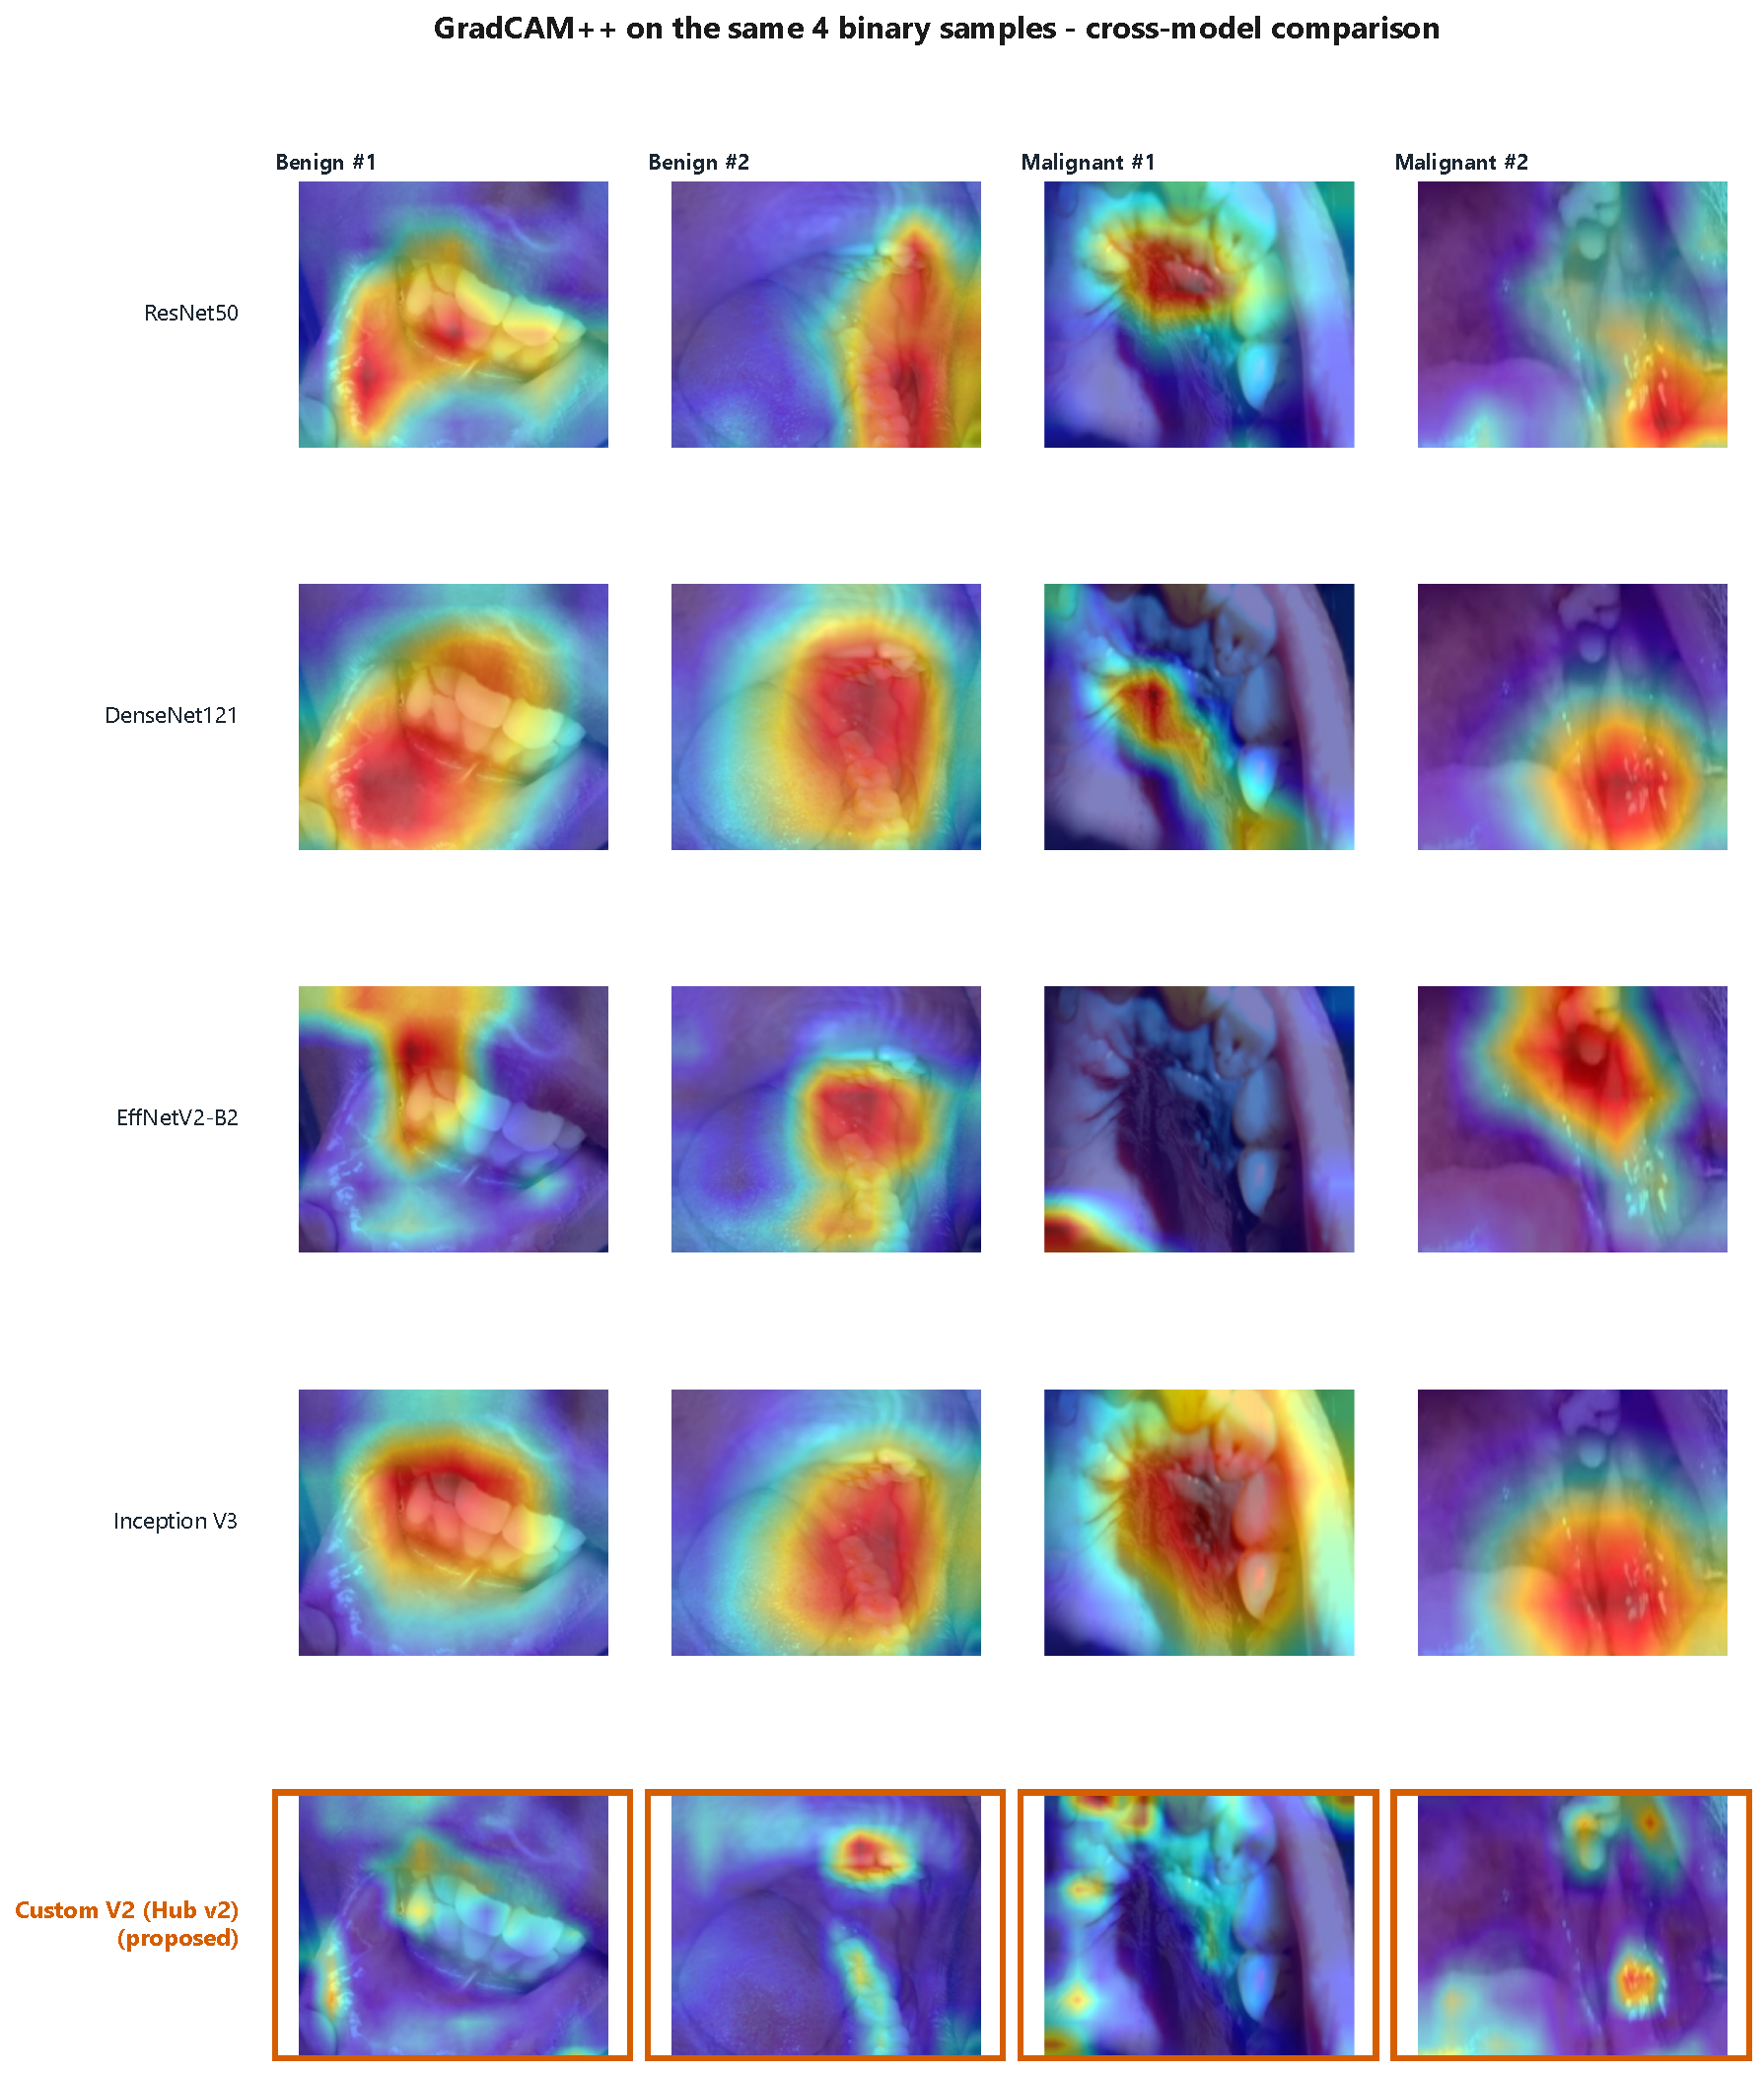
\includegraphics[width=\textwidth]{fig06_gradcam_cross_model_composite}
  \caption{Cross-model Grad-CAM++ comparison on four common binary test samples
  (two benign, two malignant). Rows correspond to ResNet50, DenseNet121,
  EfficientNet~V2-B2, Inception~V3, and the proposed Custom EfficientNet~V2
  (AttentionHub-v2, highlighted); columns correspond to the four shared inputs.
  The deterministic seed and split guarantee that each column is the same
  physical image across all rows, so differences in the heat-maps reflect the
  backbone alone. The proposed model and the two strongest baselines
  (EfficientNet~V2-B2, Inception~V3) concentrate activation on lesion tissue,
  whereas weaker backbones spread activation onto lip outlines and surrounding
  regions.}
  \label{fig:xai_cross}
\end{figure*}

\section{Discussion}\label{sec:discussion}

\subsection{What the Ablation Actually Proves}\label{subsec:what_ablation_proves}

The headline subtype number, 99.51\,\%, is the easy story. The harder
story, and the one we believe matters more for the field, is the
\textbf{role-complementarity principle}. The \texttt{bam\_triplet} cell and the
independent v2-EMA negative result, two pairings of spatial-role attention
modules reached from disjoint module sets, converge on the same 98.36\,\%
subtype ceiling, each falling below the no-attention control. It is unlikely
that two independently trained spatial-spatial configurations would land on the
same accuracy to four significant figures by chance; the probability of such a
convergence under a pure-noise null is low. We do not over-read two data points,
however: the more decisive evidence is mechanistic rather than combinatorial.
Both configurations regress \emph{beneath} the no-attention control, an
outcome a harmless redundant module could not produce, since an uninformative
module would at worst leave the representation unchanged. The convergence is
therefore better read as the signature of a systematic spatial-role conflict
than as a coincidence, and the multi-seed follow-up of
Section~\ref{subsec:future} is the proper remedy for the small sample. The
contrast with \texttt{bam\_kan} (BAM paired with the purely channel-wise KAN,
99.15\,\%) and with \texttt{triplet\_kan} (99.45\,\%) sharpens the point: a
non-spatial second module is complementary, a spatial one collides.

The consequence is that the present paper contributes not only a model but a
\emph{design rule}. When attention is added to an oral-disease classifier of
this size and on this kind of data, the modules should be paired so that they do
not both exercise the spatial role; pairing a spatial module with a purely
channel-wise module is complementary, whereas pairing two spatial modules
regresses the hub below the no-attention control. When a candidate second module
would duplicate the spatial role, the more reliable choice is to drop it. This
reframes attention-hub design from the prevailing "stack modules and report the
best configuration" practice into a measurement-driven procedure in which each
component is justified against the role taxonomy of Section~\ref{sec:prelim}.

\subsection{Comparison to Prior Multi-Class Systems}\label{subsec:vs_prior}

MODC-SET~\cite{ref22} (Section~\ref{sec:related}), the closest seven-class
result in the literature, reaches 99.32\,\% overall accuracy via a three-backbone
XGBoost ensemble. The proposed model attains 99.51\,\% subtype accuracy with a
single-stage 4.79~M parameter architecture. Because MODC-SET is evaluated on a
different seven-class collection, this is not a controlled head-to-head
comparison; we report it to situate the magnitude of the present result, not to
claim a win on a shared benchmark, and the 0.19-point delta should not be read
as a controlled accuracy advantage. The substantive contrast is methodological
rather than numerical: MODC-SET attains its accuracy by fusing features across
three large backbones, with no published ablation justifying which backbones to
ensemble or why XGBoost should serve as the meta-classifier, whereas the
accuracy of the proposed model emerges from a five-stage backbone whose only
specialized component is justified branch by branch. The two systems thus
demonstrate that high accuracy on seven-class oral disease data is attainable
by very different means; the present work shows that an efficient single-model
alternative can be reached in a principled, ablation-driven way rather than by
ensemble scale. Accordingly, the "highest subtype accuracy" claim made
throughout this paper is restricted to the controlled nine-baseline benchmark
trained here under one matched recipe; it is not asserted as a record against
the broader literature, where results obtained on different datasets and under
different protocols are not directly comparable.

Relative to the binary-screening literature~\cite{ref5,ref16,ref17}, the
proposed model maintains binary-task parity (99.06\,\% against the leading
EfficientNet~V2-B2 at 99.36\,\%) at less than half the parameter count,
while additionally delivering the seven-way subtype categorization that the
binary screeners do not address. The comparison with the segmentation
literature~\cite{ref15,ref26} is one of complementary scope rather than of
competing numbers: those systems localize lesion extent at pixel granularity,
whereas the present model identifies the disease class. The two questions are
distinct, and Section~\ref{subsec:future} returns to the prospect of combining
them.

\subsection{Why the Binary Head Plateaus}\label{subsec:binary_plateau}

Across the strongest baselines (ResNet50, Inception~V3, and
EfficientNet~V2-B2), the binary head sits within a narrow 99.1--99.4\,\%
corridor. We interpret this as a property of the data rather than of the
model: the visual gap between benign and malignant lesions is sufficiently wide
that any reasonable backbone trained from scratch resolves it almost
completely. Pushing the binary head past 99.5\,\% would require either a larger
dataset that admits harder edge cases or a task-targeted augmentation strategy;
neither is in scope here, and we do not claim a binary-task improvement.

The subtype head behaves differently. It requires the model to differentiate
among visually similar mucosal conditions, most notably MC versus OC, two
malignant carcinomas whose presentations overlap, and this is exactly where
attention-hub design has measurable leverage. The role-complementarity
principle yields its gain on the subtype head and not on the binary head
because the subtype task is the one whose residual errors are
representational rather than already saturated. The plateau on the binary head
is thus consistent with, rather than a counterexample to, the central claim of
the paper.

A clarification on the role of the dual-head construction is warranted here.
The dual-head, multi-task design is a \emph{data-utilization} mechanism: the
masked subtype loss is the means by which the binary-only DS1 collection can
contribute to the same training run as the seven-class DS2 collection, rather
than being a device claimed to raise subtype accuracy. We do not run a
single-task control (subtype-head-only training without DS1) and therefore make
no claim that joint multi-task training improves the subtype head over an
equivalent single-task model. The role-complementarity gains reported in this
paper are attributable to the AttentionHub topology, not to the multi-task
objective; isolating the contribution of joint training is left to future work,
and is recorded among the limitations below.

\subsection{Limitations}\label{subsec:limitations}

We acknowledge six limitations of the present study.

\emph{(a) Single-seed evaluation.} Each model is trained once with seed~42. For
the 0.06 percentage-point margin between AttentionHub-v2 and the best v1 cell
(\texttt{triplet\_kan}), this margin lies within the noise band of a single
run. We do not claim that v2 is \emph{statistically} better than
\texttt{triplet\_kan}; we claim that v2 is the \emph{principled} design that
the ablation forces, and that under one matched run it sets the highest subtype
number in the study.

\emph{(b) Dataset scale.} The training set is approximately 5\,500 images
across seven subtypes, small relative to natural-image benchmarks though
large relative to most oral-disease studies. We compensate through from-scratch
training (so that no ImageNet prior is smuggled in), augmentation, early
stopping, and replicated evaluation, but external validation on independent
clinics is needed before clinical deployment.

\emph{(c) Image-level only.} This work performs classification, not pixel-level
segmentation. Segmentation is a complementary direction
(Section~\ref{subsec:vs_prior}); the present model does not output lesion
masks. Bounding-box detection and pixel masks are left as future work.

\emph{(d) Training-batch timing is approximate.} The \texttt{batch\_time\_ms}
field in \texttt{performance\_metrics.json} is estimated from test-time
inference rather than measured during training. The latency numbers themselves
(mean, P50, P95) are measured correctly; only the derived "estimated epoch
time" reported alongside them is an approximation.

\emph{(e) Interpretability evidence is qualitative.} Section~\ref{sec:xai}
presents Grad-CAM++ and LIME panels and a visual alignment ranking of the
models, but the dataset carries no lesion masks and no quantitative
interpretability metric (for example deletion/insertion AUC or
pointing-game accuracy against annotated regions) is computed. The
cross-model interpretability ordering should therefore be read as indicative
rather than as a measured, falsifiable result.

\emph{(f) The dual-head contribution is not isolated.} As discussed in
Section~\ref{subsec:binary_plateau}, the dual-head multi-task design is a
data-utilization mechanism that lets the binary-only DS1 collection contribute
to training. We do not run a subtype-only single-task control, so we do not
isolate the effect of joint multi-task training on the subtype head; whether
joint training improves, leaves unchanged, or mildly degrades subtype accuracy
relative to single-task training is left to future work.

\subsection{Clinical Significance and Deployment
Considerations}\label{subsec:clinical}

The 99.51\,\% subtype accuracy reported in this study is not a clinical claim.
It is a \emph{bench-test} result on a held-out portion of a single curated
dataset, and three distinct gaps separate it from clinical deployment.

\emph{(a) Distributional gap.} The dataset's image-acquisition conditions,
patient demographics, and intra-oral-anatomy coverage are not characterized in
the published metadata. A deployment-grade screening system would require
multi-site evaluation across patient populations, imaging devices, and lighting
conditions. The proposed model's small parameter count and low inference cost
make such an evaluation tractable on commodity hardware, but the evaluation
itself has not been performed here.

\emph{(b) Decision-context gap.} The model produces a posterior over seven
classes; clinical decisions require additional inputs (history, palpation,
biopsy result) that the model does not consume. Any deployment must
therefore be framed as \emph{decision-support} rather than
\emph{decision-making}, with a clinician retaining final authority over
diagnosis and management.

\emph{(c) Calibration gap.} This work reports accuracy and F1 but does not
report calibration metrics such as Expected Calibration Error or Brier score.
For triage-style screening, where the most useful output is often a
calibrated probability that the lesion warrants biopsy, calibration becomes
more important than accuracy. We flag this as the most consequential metric the
present study does not report, and we treat its evaluation as an open
follow-up.

The proposed model is therefore released as a research artifact and as evidence
for the role-complementarity principle, not as a deployable diagnostic tool.

\subsection{Future Work}\label{subsec:future}

Five directions follow naturally from the present study.

\begin{enumerate}
  \item \textbf{Third attention slot.} Extending the role-complementarity
  principle to a \emph{third} attention slot would require a new ablation grid
  testing whether a third disjoint-role module (for example a
  frequency-domain attention, a global-context module, or a graph-based
  reasoning head) compounds the gain or whether the cascade saturates at two
  complementary modules. The principle as stated does not predict the answer.
  \item \textbf{Backbone transferability.} The v2 hub is small enough to drop
  into the larger EfficientNet~V2 family or into ResNet-style backbones;
  testing whether the same principle holds when Stage~4 sits inside a deeper or
  wider network would establish whether the rule is dataset-specific,
  architecture-specific, or general.
  \item \textbf{Multi-seed statistical evaluation.} A multi-seed run (for
  example five independent random seeds per ablation cell) would convert the
  present single-run table into a mean $\pm$ standard-deviation table, making
  within-cell variability explicit and supporting paired-sample significance
  tests between v2, \texttt{triplet\_kan}, and \texttt{full}. The principle
  predicts that the \emph{ordering} of the cells will be preserved; an
  empirical test of that prediction would strengthen the central methodological
  claim.
  \item \textbf{Hybrid classification and segmentation head.} Pairing the
  present classifier with a lightweight segmentation head that shares Stage~5
  features would recover the pixel-level information targeted by
  segmentation-only papers~\cite{ref15,ref26} while retaining the
  categorization capability targeted by classification-only
  papers~\cite{ref19,ref22}. Stage~5's 192-channel output at $7\times7$ spatial
  resolution is well suited to a small upsampling decoder.
  \item \textbf{Calibration and uncertainty.} As noted in
  Section~\ref{subsec:clinical}, calibration metrics and predictive uncertainty
  are the most consequential evaluation axes the present study does not cover.
  A follow-up applying temperature scaling, Monte-Carlo dropout, or deep
  ensembling on top of the v2 model would close this gap.
\end{enumerate}

\section{Conclusion}\label{sec:conclusion}

This paper presented a parameter-efficient five-stage convolutional
architecture for binary and multi-class oral disease classification. The
architecture departs from a standard EfficientNetV2-B0 in two deliberately
minimal ways: a custom AttentionHub replaces the donor Block-4, and the
redundant tail (Block-6 together with the convolutional head) is removed.
Through a seven-cell ablation of the AttentionHub, reinforced by a confirmatory
negative-result run, we derived a \textbf{role-complementarity principle} that
constrains how attention modules should be combined in this setting: pair
modules with disjoint functional roles, or pay a measurable accuracy penalty.
The principle forced a sequential Triplet\arrowto{}SE cascade as the proposed
\emph{AttentionHub-v2}, which under a matched fair training recipe attains
$99.06\,\%$ binary accuracy and $99.51\,\%$ subtype accuracy on a seven-class
held-out test set, the highest subtype score in a benchmark of nine standard
CNN and Transformer baselines, at $4.79$~M parameters and $0.493$~GFLOPs,
making it $2.1\times$ smaller than EfficientNet~V2-B2 and $5.0\times$ smaller
than Inception~V3, the two strongest baselines. Grad-CAM++ and LIME panels
indicate that the model attends to lesion tissue rather than to incidental
visual cues; this interpretability evidence is qualitative and is consistent
with, rather than a formal verification of, the model's clinical alignment. The
full benchmark, the ablation grid, and the explainability artifacts are released
to support reproducibility and to make the role-complementarity principle
available for re-testing on adjacent medical-imaging distributions.

\section*{Data and Code Availability}

The full source --- the training scripts (\texttt{train.py},
\texttt{custom\_efficientnet\_colab.py}), the evaluation script
(\texttt{evaluate\_final.py}), the explainability script
(\texttt{explain\_model.py}), the computational-metrics pipeline
(\texttt{compute\_model\_metrics.py}), and the ablation runner
(\texttt{run\_ablation.py}) --- is committed alongside this manuscript,
together with the per-model \texttt{classification\_metrics.json},
\texttt{performance\_metrics.json}, \texttt{training\_time.json},
\texttt{evaluation\_results.txt}, \texttt{confusion\_matrices.png}, and
\texttt{explain\_binary.png} / \texttt{explain\_subtype.png} artifacts. Dataset~1
and Dataset~2 are pre-existing curated collections; redistribution of the
original imagery is subject to the upstream dataset licenses. The model weights
for the proposed v2 model
(\texttt{results/\allowbreak custom\_\allowbreak efficientnet\_\allowbreak
v2\_\allowbreak hub\_\allowbreak v2/\allowbreak best\_\allowbreak model.pth})
and for every baseline and ablation cell are released for non-clinical research
use under the terms specified in the repository.

\section*{Conflict of Interest}

The authors declare that they have no conflict of interest relevant to the
content of this study. The proposed model is a research artifact and is not
associated with any commercial diagnostic product.

\section*{Acknowledgment}

The authors thank the maintainers of the donor model in the \texttt{timm}
library, the authors of the BAM, Triplet Attention, SE, and EMA modules whose
designs are both adopted and ablated in this work, and the developers of the
\texttt{pytorch-grad-cam}, \texttt{lime}, \texttt{thop}, and \texttt{codecarbon}
libraries on which the reproducibility provisions of this study depend.


\bibliographystyle{IEEEtran}
\bibliography{paper}

\end{document}
